\chapter{Badanie właściwości statystycznych generatora liczb losowych}

W niniejszym rozdziale przedstawiono praktyczną implementację metod statystycznych
zastosowanych do oceny jakości strumienia bitów wygenerowanego w układzie FPGA
z wykorzystaniem ring oscylatorów. Analiza została wykonana w języku Python na danych
zebranych z działającego układu. Celem badań było sprawdzenie, czy wygenerowany strumień
nie wykazuje zależności, które mogłyby świadczyć o występowaniu niepożądanych
powiązań pomiędzy kolejnymi próbkami.
Wyniki przedstawiono w postaci wykresów oraz tabel, co umożliwia ocenę
wizualną, jak i dokładne porównanie wartości liczbowych.

\section{Implementacja skryptów do akwizycji i analizy strumienia bitów}

W ramach pracy przygotowano zestaw skryptów w języku Python, których zadaniem jest
akwizycja danych z badanego układu oraz wykonanie podstawowych analiz statystycznych
zarejestrowanych strumieni bitów. Przyjęte rozwiązanie ma charakter modułowy.
Oznacza to, że część odpowiedzialna za konfigurację, wczytywanie danych, wstępne
przetwarzanie oraz właściwą analizę została rozdzielona na kilka plików, co
ułatwia rozwój kodu i wielokrotne powtarzanie eksperymentów.

\subsection{Moduł parametrów konfiguracyjnych}

Wspólna konfiguracja wszystkich programów została umieszczona w osobnym module
\texttt{user\_param.py}. Takie podejście pozwala oddzielić parametry konfiguracji
od kodu realizującego obliczenia. W praktyce oznacza to, że zmiana portu
szeregowego, liczby pobieranych bitów, maksymalnego opóźnienia autokorelacji
lub parametrów map dwuwymiarowych nie wymaga ingerencji w główną logikę programu.
Z punktu widzenia pracy badawczej jest to wygodne, ponieważ umożliwia szybkie
powtarzanie pomiarów dla różnych ustawień układu oraz porównywanie wyników
uzyskanych w różnych konfiguracjach.

Na listingu~\ref{lst:user_param_python} pokazano fragment modułu konfiguracyjnego.
Zawiera on zarówno parametry związane z transmisją UART, jak i ustawienia używane
w kolejnych etapach analizy.

\begin{lstlisting}[
    language=Python,
    caption={Fragment modułu konfiguracyjnego \texttt{user\_param.py}},
    label={lst:user_param_python},
    basicstyle=\ttfamily\small,
    breaklines=true,
    frame=single
]
UART_PORT = "COM11"
UART_BAUD = 9600
UART_TIMEOUT_S = 1.0
READ_CHUNK_SIZE = 4096
UART_BIT_ORDER = "msb"
CAPTURE_BITS = 10485760

MAX_LAG = 15
MAP2D_WORD_SIZES = (4, 8)
MAP2D_TAUS = tuple(range(9))
STEP = None
BIAS_ALPHA = 0.01
\end{lstlisting}

\subsection{Skrypt do akwizycji danych z interfejsu UART}

Pierwszym etapem procesu badawczego było zarejestrowanie strumienia bitów
generowanego przez układ sprzętowy. W tym celu opracowano skrypt
\texttt{uart\_capture.py}, którego zadaniem jest otwarcie portu szeregowego,
odbiór kolejnych porcji danych, konwersja bajtów do postaci bitowej oraz zapis
wyniku do pliku tekstowego.

Program pobiera dane w blokach o zadanym rozmiarze, a następnie rozpakowuje każdy odebrany
bajt do ośmiu bitów. Uwzględniono również możliwość wyboru kolejności bitów w bajcie,
co ma znaczenie przy współpracy z różnymi implementacjami sprzętowymi. Niezgodność
przyjętej konwencji z kolejnością wystawiania bitów przez nadajnik nie zmienia wprawdzie
zawartości informacyjnej strumienia, wprowadza jednak deterministyczną permutację pozycji
bitowych, która mogłaby zniekształcić wynik testów badających zależności lokalne.

Fragment implementacji przedstawiono w listingu\ref{lst:uart_capture_python}.
Widoczna funkcja realizuje odbiór kolejnych porcji danych i uzupełnianie tablicy
wynikowej aż do osiągnięcia zadanej długości strumienia. Tablica wynikowa alokowana jest
jednorazowo, przed rozpoczęciem odbioru, o docelowym rozmiarze \texttt{target\_bits},
dzięki czemu uniknięto wielokrotnej realokacji pamięci przy kolejnych iteracjach pętli.
Przy seriach rzędu milionów bitów ma to wymierny wpływ na czas akwizycji. Kolejne
fragmenty zapisywane są bezpośrednio w wyznaczonym wycinku tablicy, a zmienna
\texttt{collected} pełni funkcję wskaźnika bieżącej pozycji zapisu.

Istotnym elementem funkcji jest obsługa sytuacji, w których wywołanie \texttt{ser.read()}
zwraca pustą odpowiedź. Zdarza się to po upływie zdefiniowanego limitu czasu oczekiwania,
gdy generator chwilowo nie dostarcza danych, na przykład wtedy, gdy bufor modułu
ekstrakcji nie zgromadził jeszcze pełnego bajtu. Pusty odczyt nie jest wówczas traktowany
jako błąd, lecz powoduje jedynie ponowienie próby, co pozwala prowadzić akwizycję
niezależnie od zmiennej w czasie wydajności źródła entropii. Analogicznie pomijane są
porcje, z których dekoder nie zwrócił żadnych bitów.

Ostatni odebrany blok jest z reguły dłuższy niż liczba bitów pozostających do zebrania,
ponieważ rozmiar bloku nie musi być dzielnikiem zadanej długości serii. Zastosowanie
zmiennych \texttt{remaining} i \texttt{take} zapewnia przycięcie nadmiarowej części
i zakończenie akwizycji dokładnie na zadanej liczbie bitów. Ma to znaczenie dla
poprawności dalszej analizy, ponieważ część testów pakietu NIST wymaga strumienia
o ściśle określonej długości, a seria dłuższa od deklarowanej mogłaby prowadzić do
niejednoznacznego podziału danych na bloki.

\begin{lstlisting}[
    language=Python,
    caption={Fragment skryptu \texttt{uart\_capture.py} odpowiedzialny za akwizycję bitów},
    label={lst:uart_capture_python},
    basicstyle=\ttfamily\small,
    breaklines=true,
    frame=single
]
def capture_one_series(ser: serial.Serial, target_bits: int, 
    chunk_size: int, bit_order: str, 
    progress_every_percent: int,) -> np.ndarray:

    bits = np.empty(target_bits, dtype=np.uint8)
    collected = 0

    while collected < target_bits:
        raw = ser.read(chunk_size)
        if not raw:
            continue

        chunk_bits = decode_uart_chunk_to_bits(raw=raw, 
                     bit_order=bit_order)
        if chunk_bits.size == 0:
            continue

        remaining = target_bits - collected
        take = min(remaining, int(chunk_bits.size))
        bits[collected : collected + take] = chunk_bits[:take]
        collected += take

    return bits
\end{lstlisting}

\subsection{Skrypt wybielający z wykorzystaniem metody Von Neumanna}

Po rejestracji danych zastosowano dodatkowy etap wstępnego przetwarzania,
wybrano wybielanie strumienia bitów metodą Von Neumanna. Celem tego
algorytmu jest ograniczenie wpływu biasu, czyli nierównowagi pomiędzy liczbą
zer i jedynek, bez potrzeby stosowania bardziej złożonych metod korekcji.

Strumień wejściowy dzielony jest na kolejne
pary bitów. Jeżeli w parze wystąpią dwa identyczne bity, para jest odrzucana.
Jeżeli bity są różne, do strumienia wyjściowego przepisywany jest pierwszy bit
z tej pary. W efekcie otrzymywany jest nowy ciąg o lepszych właściwościach
statystycznych, chociaż zazwyczaj krótszy od ciągu wejściowego. Skuteczność metody
opiera się na założeniu, że kolejne bity strumienia są statystycznie niezależne,
a jedynym jego defektem jest stałe odchylenie prawdopodobieństwa. Przy spełnieniu
tego warunku obie różne pary występują z jednakowym prawdopodobieństwem niezależnie
od wartości biasu, co gwarantuje idealną równowagę strumienia wyjściowego. Ceną
jest redukcja długości ciągu, w przypadku źródła nieobciążonego do około jednej
czwartej liczby bitów wejściowych, a dla źródła silnie odchylonego jeszcze wyraźniejsza.
Z punktu widzenia pracy badawczej rozwiązanie to jest użyteczne, ponieważ pozwala
porównać wyniki analizy przed i po wybielaniu danych. Implementację tej operacji
przedstawiono na listingu\ref{lst:von_neumann_python}.

\begin{lstlisting}[
    language=Python,
    caption={Fragment skryptu \texttt{von\_neumann.py} realizującego wybielanie bitów},
    label={lst:von_neumann_python},
    basicstyle=\ttfamily\small,
    breaklines=true,
    frame=single
]
def von_neumann_whiten(bits: np.ndarray) -> np.ndarray:
    pair_count = len(bits) // 2
    if pair_count == 0:
        return np.empty(0, dtype=np.uint8)

    pairs = bits[: 2 * pair_count].reshape(pair_count, 2)
    different = pairs[:, 0] != pairs[:, 1]

    return pairs[different, 0].astype(np.uint8, copy=False)
\end{lstlisting}

Implementację zrealizowano w postaci wektorowej, bez jawnej pętli po parach bitów.
Liczba pełnych par wyznaczana jest przez dzielenie całkowite długości strumienia,
a przy nieparzystej liczbie bitów ostatni z nich jest pomijany, ponieważ nie tworzy
kompletnej pary. Operacja \texttt{reshape} przekształca jednowymiarową tablicę bitów
w macierz o dwóch kolumnach, w której każdy wiersz odpowiada jednej analizowanej parze.
Porównanie obu kolumn daje logiczną maskę wskazującą pary o różnych wartościach,
która następnie służy do wybrania z pierwszej kolumny wyłącznie bitów spełniających
warunek zachowania. Takie podejście pozwala przetworzyć całą serię pomiarową
w kilku operacjach na tablicach, co przy strumieniach rzędu milionów bitów jest
zauważalnie szybsze od przetwarzania iteracyjnego.

Wybielanie realizowane jest po stronie komputera, na danych już zarejestrowanych,
a nie w strukturze układu FPGA. Rozwiązanie takie przyjęto celowo, ponieważ umożliwia
ono wielokrotną analizę tej samej serii pomiarowej przy różnych ustawieniach przetwarzania
oraz bezpośrednie porównanie strumienia surowego z wybielonym. Warunek zwracający
tablicę pustą dla strumienia krótszego od dwóch bitów zabezpiecza dalsze etapy analizy
przed błędem przy przetwarzaniu niekompletnych serii.

\subsection{Skrypt do wyznaczania autokorelacji}

Skrypt \texttt{autocorrelation.py}, służy do oceny zależności pomiędzy
bitami oddzielonymi określonym opóźnieniem. Badanie autokorelacji jest istotne,
ponieważ pozwala sprawdzić, czy kolejne próbki są od siebie niezależne.
W idealnym generatorze liczb losowych wartości autokorelacji dla opóźnień
większych od zera powinny być bliskie zeru.

W analizowanym rozwiązaniu strumień wejściowy w postaci \texttt{0}/\texttt{1}
jest najpierw przekształcany do postaci \texttt{-1}/\texttt{+1}. Zabieg ten sprowadza
wartość oczekiwaną strumienia nieobciążonego do zera, dzięki czemu iloczyn dwóch
próbek przyjmuje wartość dodatnią przy zgodności bitów i ujemną przy ich
niezgodności, a średnia z takich iloczynów wprost wyraża siłę i znak zależności.
Przy oryginalnym kodowaniu zerojedynkowym iloczyn byłby niezerowy wyłącznie dla par
jedynek, co czyniłoby miarę nieczułą na znaczną część możliwych zależności. Następnie
dla każdego opóźnienia wyznaczana jest średnia wartość iloczynu dwóch fragmentów
ciągu, z których jeden jest przesunięty względem drugiego. Program realizuje
obliczenia dla opóźnień od zera do wartości określonej przez parametr
\texttt{MAX\_LAG}. Dodatkowo generowane są wykresy oraz tabela z obliczonymi
wartościami, co ułatwia interpretację wyników.

Przykładową implementację funkcji obliczającej autokorelację przedstawiono
na listingu\ref{lst:autocorrelation_python}.

\begin{lstlisting}[
    language=Python,
    caption={Fragment skryptu \texttt{autocorrelation.py} do wyznaczania autokorelacji},
    label={lst:autocorrelation_python},
    basicstyle=\ttfamily\small,
    breaklines=true,
    frame=single
]
def autocorrelation(bits: np.ndarray, max_lag: int) -> np.ndarray:
    if len(bits) < max_lag + 1:
        raise ValueError("Not enough bits for MAX_LAG.")

    x = bits.astype(np.int8) * 2 - 1
    ac = np.empty(max_lag + 1, dtype=np.float64)

    for lag in range(max_lag + 1):
        a = x[: len(x) - lag]
        b = x[lag:]
        ac[lag] = np.mean(a * b)

    return ac
\end{lstlisting}

Dla każdego opóźnienia tworzone są dwa wycinki tego samego ciągu, przesunięte
względem siebie o zadaną liczbę pozycji i skrócone do wspólnej długości, tak aby
uśrednianie obejmowało wyłącznie pary o pełnym pokryciu. Wynikiem funkcji jest
tablica o długości \texttt{MAX\_LAG+1}, w której pierwszy element odpowiada opóźnieniu
zerowemu. Element ten z definicji przyjmuje wartość jedności, ponieważ każda próbka
mnożona jest wówczas przez siebie samą, a wobec kodowania \texttt{-1}/\texttt{+1}
iloczyn ten jest zawsze dodatni. Stanowi to wygodny punkt odniesienia oraz prosty
test poprawności działania funkcji.

Interpretacja pozostałych wartości wymaga uwzględnienia rozrzutu statystycznego.
Nawet dla źródła idealnie losowego wyznaczone współczynniki nie są dokładnie zerowe,
lecz wahają się w otoczeniu zera z odchyleniem standardowym rzędu odwrotności
pierwiastka z liczby analizowanych par. Przy serii o długości miliona bitów oznacza
to typowe odchylenia rzędu jednej tysięcznej, wobec czego dopiero wartości istotnie
przekraczające ten poziom świadczą o rzeczywistej zależności między próbkami.
W przypadku badanego generatora szczególnej uwagi wymagają opóźnienia odpowiadające
liczbie oscylatorów oraz wielokrotności długości bajtu, ponieważ ewentualna
periodyczność wynikająca ze stałej kolejności zapisu kanałów do bufora ujawniłaby się
właśnie w tych miejscach.

Zastosowany algorytm ma złożoność proporcjonalną do iloczynu długości strumienia
i maksymalnego opóźnienia, co przy dużych wartościach parametru \texttt{MAX\_LAG}
może być kosztowne obliczeniowo. Dla rozważanych zakresów opóźnień narzut ten
pozostaje jednak akceptowalny, a bezpośrednia postać obliczeń jest czytelniejsza
i łatwiejsza do weryfikacji niż realizacja z użyciem szybkiej transformaty Fouriera.

\subsection{Skrypt do tworzenia dwuwymiarowych map opóźnień}

Do bardziej zaawansowanej analizy zależności w danych wykorzystano skrypt
\texttt{map2d\_analysis.py}. Jego zadaniem jest budowa dwuwymiarowych map
opóźnień, które pozwalają ocenić strukturę badanego strumienia z większą
dokładnością niż proste zliczanie zer i jedynek, czy autokorelacja pierwszego
rzędu. Miary jednowymiarowe wykrywają wyłącznie zależności liniowe pomiędzy
pojedynczymi bitami, wobec czego strumień może uzyskać poprawny wynik testu
autokorelacji, zawierając jednocześnie wyraźne prawidłowości na poziomie całych
słów.

Działanie programu polega na podziale strumienia bitów na słowa o zadanej długości,
na przykład 4 lub 8-bitowe, a następnie na utworzeniu par \((w[n], w[n+\tau])\)
dla wybranych wartości opóźnienia \(\tau\). Dla takich par wyznaczany jest
histogram dwuwymiarowy, który można interpretować jako mapę gęstości występowania
określonych kombinacji słów. Dla źródła idealnie losowego wszystkie kombinacje są
jednakowo prawdopodobne, wobec czego mapa powinna mieć charakter równomiernego
szumu, bez wyróżnionych linii, skupień ani obszarów pustych. Struktury regularne
widoczne na mapie świadczą o tym, że wartość danego słowa niesie informację
o wartości słowa następnego. Dodatkowo skrypt oblicza kilka prostych parametrów
opisujących taką mapę, między innymi liczbę zajętych komórek histogramu,
udział wypełnienia siatki oraz udział punktów leżących na przekątnej.
Pierwsze dwa parametry pozwalają stwierdzić, czy generator wykorzystuje całą
dostępną przestrzeń wartości, natomiast udział punktów na przekątnej wskazuje,
jak często słowo powtarza się po zadanym opóźnieniu, co jest bezpośrednią miarą
skłonności układu do zapadania w stany okresowe.
Wyniki te są zapisywane zarówno w postaci wykresów, jak i tabel zbiorczych.

Przykładowy fragment kodu generującego mapę 2D przedstawiono
w Listingu~\ref{lst:map2d_python}.

\begin{lstlisting}[
    language=Python,
    caption={Fragment skryptu \texttt{map2d\_analysis.py} generującego mapę opóźnień 2D},
    label={lst:map2d_python},
    basicstyle=\ttfamily\small,
    breaklines=true,
    frame=single
]
def plot_delay_map_2d(
        x: np.ndarray, y: np.ndarray,
        bit_count: int, word_count: int,
        word_size: int, tau: int,
        bins: int | None = None,
        output: Path | None = None,
    ) -> dict[str, int | float]: 

    max_val = 2**word_size
    if bins is None:
        bins = min(max_val, 256)

    hist, xedges, yedges = np.histogram2d(x, y, bins=bins,
        range=[[0, max_val], [0, max_val]],
    )

    occupied_bins = int(np.count_nonzero(hist))
    fill_ratio = occupied_bins / int(hist.size)
    diagonal_share = float(np.trace(hist)) / len(x)

    return {
        "word_size": word_size,
        "tau": tau,
        "occupied_bins": occupied_bins,
        "fill_ratio": fill_ratio,
        "diagonal_share": diagonal_share,
    }
\end{lstlisting}

Zakres histogramu wyznaczany jest na podstawie długości słowa i obejmuje pełny
przedział możliwych wartości. Liczba przedziałów podziału ustalana jest domyślnie
jako mniejsza z dwóch wartości: liczby możliwych kombinacji oraz górnego
ograniczenia równego 256. Dla słów czterobitowych oznacza to podział dokładnie
odwzorowujący pojedyncze wartości, natomiast dla słów dłuższych kilka sąsiednich
wartości trafia do wspólnej komórki. Ograniczenie to jest niezbędne z uwagi na
rozmiar histogramu, który rośnie z kwadratem liczby przedziałów, wymaga jednak
uwzględnienia przy interpretacji parametru wypełnienia. Przy zbyt dużej liczbie
komórek w stosunku do długości serii pomiarowej niski współczynnik wypełnienia
wynika bowiem z niedostatecznej liczby próbek, a nie z wadliwości generatora.

Udział punktów leżących na przekątnej wyznaczany jest jako iloraz śladu macierzy
histogramu i całkowitej liczby analizowanych par. Interpretacja tej wielkości
wymaga porównania z wartością oczekiwaną dla źródła losowego, która jest równa
odwrotności liczby przedziałów podziału. Wartość istotnie wyższa świadczy
o powtarzalności słów, natomiast wyraźnie niższa może wskazywać na mechanizm
wykluczający powtórzenia, co również stanowi odstępstwo od losowości.

Zastosowanie map dwuwymiarowych było przydatne z praktycznego punktu widzenia,
ponieważ pozwalało wykrywać nie tylko prosty bias, ale również bardziej złożone
zależności pomiędzy kolejnymi fragmentami badanego ciągu.

\subsection{Skrypt do wyznaczania odchylenia rozkładu bitów}

Skrypt \texttt{bias.py} służy do oceny najbardziej podstawowej właściwości strumienia
losowego, jaką jest równowaga pomiędzy liczbą zer i jedynek. Dla źródła idealnego
prawdopodobieństwo wystąpienia obu wartości jest jednakowe, wobec czego udział jedynek
w dostatecznie długim strumieniu powinien być bliski jednej drugiej. Odstępstwo od tej
wartości, określane jako odchylenie rozkładu lub bias, jest w przypadku generatorów
sprzętowych zjawiskiem oczekiwanym i wynika między innymi z niesymetrycznych czasów
propagacji zbocza narastającego i opadającego w łańcuchu inwerterów oraz z niezerowego
współczynnika wypełnienia próbkowanego przebiegu.

Program wczytuje strumienie bitów z pliku tekstowego, sprawdza poprawność danych
wejściowych, a następnie dla każdego strumienia wyznacza liczbę zer i jedynek,
prawdopodobieństwa $P(0)$ oraz $P(1)$, wartość biasu zdefiniowaną jako $P(1)-0{,}5$,
średnią po odwzorowaniu bitów do zbioru $\{-1,+1\}$, a także wartość $p$ dla testu
monobitowego. Poziom istotności zadawany jest w konfiguracji parametrem
\texttt{BIAS\_ALPHA}, dzięki czemu procedurę można powtarzać dla różnych ustawień.
Fragment implementacji przedstawiono na listingu~\ref{lst:bias_python}.

\begin{lstlisting}[
    language=Python,
    caption={Fragment skryptu realizującego analizę biasu strumienia bitów},
    label={lst:bias_python},
    basicstyle=\ttfamily\small,
    breaklines=true,
    frame=single
]
def analyze_bitstream(bits: np.ndarray, bitstream_idx: int, bitstream_count: int) -> dict[str, float | int | bool]:
    total_bits = len(bits)
    one_count = int(np.count_nonzero(bits))
    zero_count = total_bits - one_count
    p_one = one_count / total_bits
    p_zero = zero_count / total_bits
    bias_01 = p_one - 0.5
    mean_pm1 = 2.0 * p_one - 1.0
    sigma_bias = 0.5 / sqrt(total_bits)
    s_n = one_count - zero_count
    s_obs = abs(s_n) / sqrt(total_bits)
    p_value = erfc(s_obs / sqrt(2.0))
    passed = p_value >= BIAS_ALPHA

    return {
        "bitstream_idx": bitstream_idx, "total_bits": total_bits,
        "zero_count": zero_count, "one_count": one_count,
        "p_zero": p_zero, "p_one": p_one,
        "bias_01": bias_01, "mean_pm1": mean_pm1,
        "sigma_bias": sigma_bias, "p_value": p_value,
        "passed": passed,
    }
\end{lstlisting}

Liczba jedynek wyznaczana jest jednym wywołaniem funkcji zliczającej elementy niezerowe,
co przy strumieniach rzędu milionów bitów jest znacznie szybsze od przetwarzania
iteracyjnego. Obie zwracane miary odchylenia, $P(1)-0{,}5$ oraz średnia w kodowaniu
$\{-1,+1\}$, opisują to samo zjawisko i różnią się wyłącznie skalą, przy czym druga
z nich jest dokładnie dwukrotnie większa. Podanie obu wynika z tego, że pierwsza jest
przyjęta w opisach generatorów sprzętowych, natomiast druga pojawia się w kontekście
analizy korelacyjnej, gdzie stosuje się to samo odwzorowanie bitów.

Kluczowym elementem funkcji jest realizacja testu monobitowego zgodnie z metodyką
pakietu NIST. Wyznaczana jest nadwyżka jedynek nad zerami, normowana pierwiastkiem
z długości strumienia, a otrzymana statystyka przeliczana jest na wartość $p$ przy użyciu
uzupełniającej funkcji błędu. Wartość ta określa prawdopodobieństwo zaobserwowania
odchylenia co najmniej tak dużego, jak stwierdzone, przy założeniu że źródło jest
idealnie zrównoważone. Normowanie długością serii jest tu istotne dla interpretacji
wyników: ta sama wartość biasu daje tym mniejszą wartość $p$, im dłuższa jest analizowana
seria, ponieważ dłuższa próba pozwala wykryć coraz subtelniejsze odchylenia. Wyznaczane
dodatkowo odchylenie standardowe $\sigma = 1/(2\sqrt{N})$ służy jako miara odniesienia
i pozwala wyrazić stwierdzone odstępstwo w jednostkach naturalnego rozrzutu
statystycznego.

\subsection{Podsumowanie}

Przygotowany zestaw skryptów tworzy spójne środowisko do badań nad jakością
strumienia bitów generowanego przez badany układ. Skrypt \texttt{uart\_capture.py}
odpowiada za akwizycję danych, moduł \texttt{user\_param.py} zapewniają wspólną 
konfigurację, \texttt{von\_neumann.py} realizuje wstępne wybielanie strumienia, natomiast
\texttt{autocorrelation.py}, \texttt{bias.py} oraz \texttt{map2d\_analysis.py}
służą do właściwej analizy statystycznej. Taki podział ułatwia zarówno
powtarzanie eksperymentów, jak i porównywanie wyników uzyskanych dla różnych
konfiguracji generatora.

Przyjęta struktura odzwierciedla naturalną kolejność przetwarzania danych,
od akwizycji, przez opcjonalne wybielanie, aż do analizy statystycznej. Rozdzielenie
tych etapów sprawia, że pojedyncza seria pomiarowa, po jednorazowym zarejestrowaniu,
może być poddawana wielokrotnej analizie przy różnych ustawieniach parametrów, bez
konieczności ponownego uruchamiania układu sprzętowego. Wydzielenie parametrów
konfiguracyjnych do osobnego modułu zapewnia ponadto, że wszystkie skrypty
operują na jednakowych ustawieniach długości serii, kolejności bitów oraz
zakresów analizy, co jest warunkiem porównywalności wyników uzyskanych
w kolejnych eksperymentach.

Zastosowane miary są wobec siebie komplementarne. Analiza biasu ocenia rozkład
wartości pojedynczych bitów, autokorelacja bada zależności między bitami
oddalonymi o zadaną liczbę pozycji, natomiast mapy dwuwymiarowe ujawniają
prawidłowości na poziomie całych słów. Dopiero łączne rozpatrzenie wyników
wszystkich trzech metod, dla strumienia surowego oraz wybielonego, pozwala
formułować wnioski na temat jakości badanego źródła entropii.

\subsection{Zestawienie parametrów badanych konfiguracji}

Wszystkie omówione pomiary wykonano na tej samej płytce rozwojowej i przy jednakowej
długości serii pomiarowej wynoszącej $10\,485\,760$ bitów, co odpowiada dziesięciu
mebibajtom danych. Konfiguracje różniły się liczbą użytych oscylatorów, sposobem ich
rozmieszczenia w strukturze układu, obecnością operacji XOR na wyjściach oraz
zastosowaniem wybielania po stronie komputera. Zestawienie tych parametrów przedstawiono
w tabeli~\ref{tab:konfiguracje}.

\begin{table}[htbp]
    \centering
    \caption{Parametry badanych konfiguracji generatora}
    \label{tab:konfiguracje}
    \small
    \begin{tabular}{clcccc}
        \toprule
        Nr & Rozmieszczenie & Liczba RO & Kanały & XOR & Wybielanie \\
        \midrule
        1 & automatyczne & 8  & 8 & nie  & nie \\
        2 & ręczne       & 8  & 8 & nie  & nie \\
        3 & ręczne       & 16 & 8 & tak  & nie \\
        4 & ręczne       & 16 & 8 & tak  & tak \\
        \bottomrule
    \end{tabular}
\end{table}

Liczba stopni inwersji poszczególnych oscylatorów została ustalona w tablicy stałych
\texttt{STAGE\_TABLE} i wynosi kolejno od 7 do 37, ze skokiem równym dwa. Zastosowanie
wyłącznie wartości nieparzystych jest warunkiem koniecznym wystąpienia oscylacji,
ponieważ przy parzystej liczbie inwerterów pętla sprzężenia zwrotnego realizowałaby
funkcję tożsamości i układ ustaliłby się w jednym ze stanów stabilnych. Zróżnicowanie
długości łańcuchów prowadzi natomiast do zróżnicowania częstotliwości pracy, która maleje
w przybliżeniu odwrotnie proporcjonalnie do liczby stopni. Zapobiega to sytuacji,
w której wszystkie oscylatory pracowałyby z jednakową częstotliwością nominalną, co
zwiększałoby ryzyko ich wzajemnej synchronizacji i ograniczyłoby efektywną liczbę
niezależnych źródeł szumu.

W konfiguracjach obejmujących osiem oscylatorów wykorzystywanych jest osiem pierwszych
pozycji tablicy, a więc łańcuchy o długościach od 7 do 21 stopni. W konfiguracjach
z szesnastoma oscylatorami wykorzystywana jest cała tablica, przy czym wyjścia łączone są
w pary operacją XOR według schematu 0--1, 2--3 i tak dalej, do pary 14--15. Do modułu
ekstrakcji entropii doprowadzonych jest zatem w każdym przypadku osiem sygnałów,
co oznacza, że przepustowość generatora nie zależy od liczby zaimplementowanych
oscylatorów. Warto zwrócić uwagę, że przyjęty schemat parowania zestawia zawsze łańcuch
krótszy z łańcuchem o dwa stopnie dłuższym, a więc o najbliższej możliwej częstotliwości
w obrębie zestawu.

Rozmieszczenie oscylatorów w konfiguracjach 2--4 narzucono ręcznie za pomocą ograniczeń
\texttt{LOC} oraz \texttt{BEL} zapisanych w pliku ograniczeń projektu. Pierwsze
z~ograniczeń przypisuje dany element logiczny do konkretnego bloku \texttt{SLICE},
drugie wskazuje wybrany generator funkcji w obrębie tego bloku. Takie podejście pozwala
uzyskać powtarzalną implementację, niezależną od kolejnych przebiegów narzędzia
rozmieszczającego, co jest warunkiem porównywalności pomiarów wykonanych w~różnym czasie.
Obszary zajmowane przez poszczególne oscylatory zestawiono w~tabeli~\ref{tab:rozm},
podając zakres współrzędnych bloków, w~których umieszczono należące do nich generatory
funkcji.

\begin{table}[htbp]
    \centering
    \caption{Liczba stopni inwersji oraz obszar rozmieszczenia poszczególnych oscylatorów}
    \label{tab:rozm}
    \small
    \begin{tabular}{ccccccc}
        \toprule
        RO & Stopnie & Obszar & \phantom{aa} & RO & Stopnie & Obszar \\
        \midrule
        0 & 7  & X40Y1--X40Y2   & & 8  & 23 & X0Y48--X2Y49   \\
        1 & 9  & X0Y99--X1Y99   & & 9  & 25 & X16Y48--X19Y49 \\
        2 & 11 & X6Y97--X7Y97   & & 10 & 27 & X35Y40--X40Y42 \\
        3 & 13 & X22Y0--X23Y2   & & 11 & 29 & X23Y87--X28Y89 \\
        4 & 15 & X19Y15--X22Y16 & & 12 & 31 & X5Y37--X8Y38   \\
        5 & 17 & X31Y67--X33Y68 & & 13 & 33 & X10Y63--X15Y64 \\
        6 & 19 & X31Y97--X32Y99 & & 14 & 35 & X33Y24--X36Y26 \\
        7 & 21 & X4Y73--X7Y74   & & 15 & 37 & X6Y84--X10Y87  \\
        \bottomrule
    \end{tabular}
\end{table}

\begin{figure}[htbp]
    \centering
    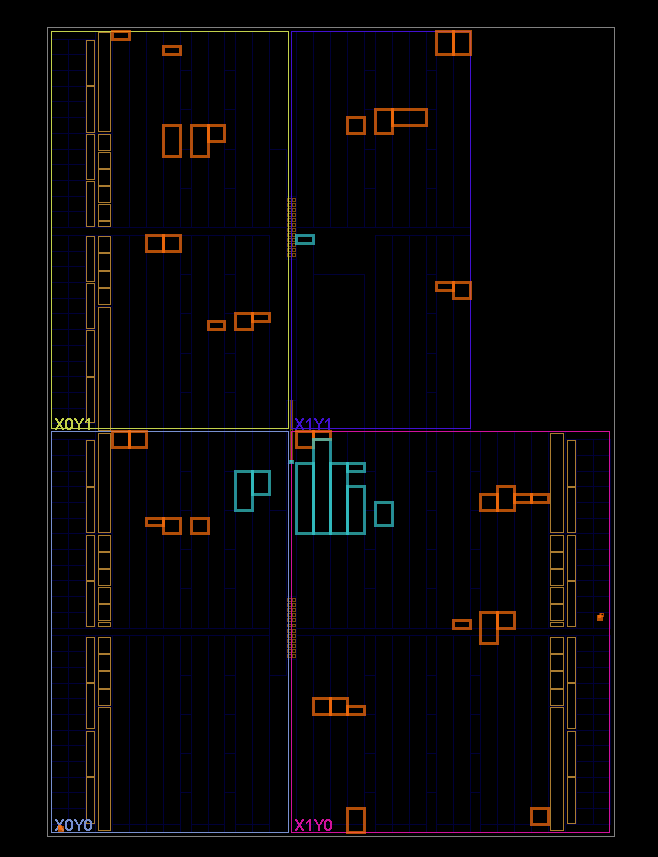
\includegraphics[width=0.7\textwidth]{gfx/ro_trng_xor_place_and_route.png}
    \caption{Widok struktury układu Spartan-7 po etapie rozmieszczenia i trasowania dla
    konfiguracji z 16 oscylatorami. Kolorem pomarańczowym oznaczono zasoby zajęte przez
    oscylatory pierścieniowe, kolorem błękitnym logikę modułu ekstrakcji entropii oraz
    nadajnika UART. Podpisy w narożnikach wskazują granice regionów zegarowych}
    \label{fig:place_and_route}
\end{figure}

Efekt zastosowanych ograniczeń przedstawiono na rysunku~\ref{fig:place_and_route},
obrazującym rozmieszczenie logiki w strukturze układu po etapie implementacji.
Oscylatory zajmują niewielkie, wyraźnie odseparowane grupy bloków rozproszone po całej
powierzchni logiki programowalnej, obejmujące wszystkie cztery regiony zegarowe układu.
Widoczne jest przy tym zróżnicowanie rozmiaru poszczególnych grup, wynikające
bezpośrednio z liczby stopni inwersji: łańcuchy najkrótsze mieszczą się w obrębie jednego
lub dwóch bloków, natomiast łańcuchy o kilkudziesięciu stopniach zajmują kilka bloków
sąsiadujących w poziomie. Zwarta grupa w centralnej części struktury odpowiada logice
synchronicznej projektu, a więc modułowi ekstrakcji entropii, nadajnikowi UART oraz
rejestrom synchronizującym.

Podział struktury na regiony zegarowe jest istotny z punktu widzenia niezależności
źródeł entropii, ponieważ każdy region posiada odrębne zasoby dystrybucji sygnału
zegarowego oraz własne punkty przyłączenia do sieci zasilania. Rozmieszczenie
oscylatorów w różnych regionach zwiększa zatem prawdopodobieństwo, że lokalne
zaburzenia napięcia zasilania, wywołane przełączaniem logiki synchronicznej, będą
oddziaływać na poszczególne pierścienie w sposób nieskorelowany. Jednocześnie warto
zaznaczyć, że żaden z oscylatorów nie został umieszczony w bezpośrednim sąsiedztwie
logiki synchronicznej, co ogranicza wpływ jej okresowej aktywności na częstotliwość
generowanych przebiegów.

Przyjęte rozmieszczenie obejmuje praktycznie cały obszar logiki programowalnej układu,
od bloków o najniższych współrzędnych po skrajne bloki w~narożnikach struktury. Oscylatory
tworzące jedną parę połączoną operacją XOR umieszczono w~odległych obszarach, przy czym
w~skrajnym przypadku pary 0--1 są to przeciwległe narożniki układu. Wyjątkiem jest para
8--9, której oba oscylatory znajdują się w~tym samym pasie poziomym, w~odległości około
szesnastu bloków. Konfiguracja ta jest zatem najbardziej narażona na wzajemne
oddziaływanie obu struktur i stanowi potencjalne źródło osłabienia skuteczności operacji
XOR dla tego kanału.

Łączne zapotrzebowanie na zasoby logiczne wynika bezpośrednio z~liczby stopni inwersji.
Każdy stopień realizowany jest przez jeden generator funkcji, a~dodatkowy generator
w~każdym oscylatorze pełni funkcję bramkowania sygnału wyjściowego sygnałem zezwolenia.
Konfiguracje z~ośmioma oscylatorami wymagają zatem 120 generatorów funkcji, natomiast
konfiguracje z~szesnastoma oscylatorami 368, nie licząc logiki modułu ekstrakcji entropii
oraz nadajnika UART. Struktury oscylatorów objęto atrybutami \texttt{dont\_touch} oraz
\texttt{keep}, co uniemożliwia narzędziu syntezy usunięcie łańcucha inwerterów jako
logiki redundantnej lub jego uproszczenie do pojedynczej negacji.

\FloatBarrier

\section{Badanie autokorelacji uzyskanych strumieni bitów}

Jednym z pierwszych wykonanych badań była analiza autokorelacji wygenerowanego strumienia
bitów. W praktyce test ten został użyty do sprawdzenia, czy kolejne bity wygenerowane w
układzie FPGA nie wykazują krótkookresowych zależności, które mogłyby wynikać z architektury
układu, sposobu próbkowania lub zbyt małego poziomu entropii na wejściu bloku
odpowiedzialnego za generację bitów. Do badania wykorzystano zapisany strumień o długości
$10\,485\,760$ bitów. Analiza została wykonana dla opóźnień od 0 do 15. Obliczenia
zrealizowano w języku Python, a skrypt został przygotowany tak, aby automatycznie wyznaczać
współczynniki autokorelacji oraz zapisywać wyniki w postaci wykresu i tabeli.

\subsection{Wyniki pomiaru dla 8 oscylatorów bez wybielania}

Przebieg współczynnika autokorelacji w funkcji opóźnienia przedstawiono na
rysunku~\ref{fig:autokorelacja_bitstream}, natomiast dokładne wartości liczbowe zestawiono
w tabeli~\ref{tab:autokorelacja_wyniki}.

\begin{figure}[htbp]
    \centering
    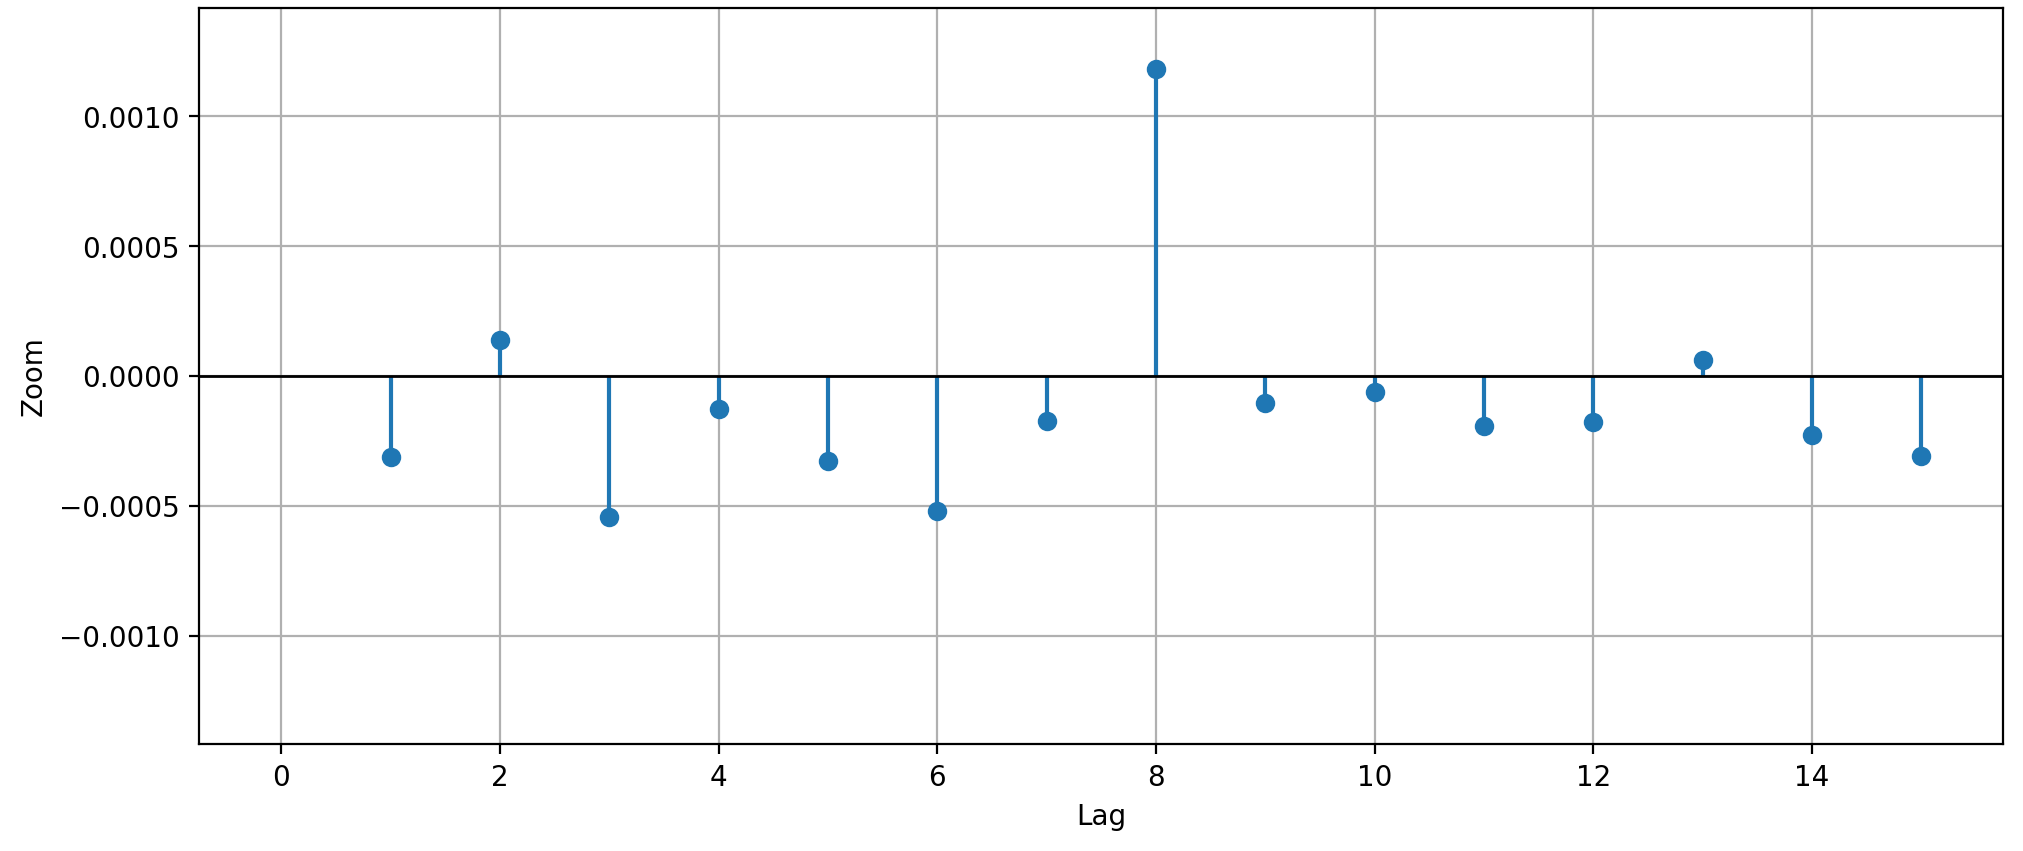
\includegraphics[width=0.9\textwidth]{gfx/no_wh_ac.png}
    \caption{Autokorelacja badanego strumienia bitów dla opóźnień od 0 do 15}
    \label{fig:autokorelacja_bitstream}
\end{figure}

\begin{table}[htbp]
    \centering
    \caption{Wartości współczynników autokorelacji dla badanego strumienia bitów}
    \label{tab:autokorelacja_wyniki}
    \small
    \begin{tabular}{rrrr}
        \toprule
        Opóźnienie & $R$ & Opóźnienie & $R$ \\
        \midrule
        0 & $+1{,}000000$ & 8  & $+0{,}001182$ \\
        1 & $-0{,}000309$ & 9  & $-0{,}000102$ \\
        2 & $+0{,}000139$ & 10 & $-0{,}000060$ \\
        3 & $-0{,}000544$ & 11 & $-0{,}000192$ \\
        4 & $-0{,}000127$ & 12 & $-0{,}000176$ \\
        5 & $-0{,}000326$ & 13 & $+0{,}000061$ \\
        6 & $-0{,}000520$ & 14 & $-0{,}000226$ \\
        7 & $-0{,}000173$ & 15 & $-0{,}000306$ \\
        \bottomrule
    \end{tabular}
\end{table}

Na podstawie otrzymanych wyników można stwierdzić, że poza oczywistą wartością równą
jedności dla opóźnienia zerowego wszystkie współczynniki autokorelacji pozostają bliskie
zeru, nie przekraczając wartości bezwzględnej $1{,}2 \cdot 10^{-3}$. W badanym zakresie nie
zaobserwowano narastającego trendu ani wartości sugerujących silną zależność pomiędzy
kolejnymi bitami.

Interpretacja tych wielkości wymaga jednak odniesienia do rozrzutu statystycznego. Dla
strumienia w pełni losowego o długości $N$ bitów wyznaczone współczynniki wahają się wokół
zera z odchyleniem standardowym w przybliżeniu równym $1/\sqrt{N}$, co dla badanej serii
daje wartość $\sigma \approx 3{,}1 \cdot 10^{-4}$. Zdecydowana większość odnotowanych
wartości nie przekracza dwukrotności tego poziomu i mieści się w granicach naturalnych
fluktuacji.

Wyjątkiem jest opóźnienie równe 8, dla którego uzyskano $R = 0{,}001182$, czyli blisko
czterokrotność odchylenia standardowego. Wartość ta odstaje od pozostałych, a jej położenie
nie jest przypadkowe, ponieważ opóźnienie 8 odpowiada zarówno liczbie oscylatorów
pierścieniowych, jak i długości bajtu wystawianego przez moduł ekstrakcji entropii. Bity
zapisywane są do bufora w stałej kolejności numerów kanałów, wobec czego pozycje odległe
o osiem miejsc pochodzą statystycznie częściej z tego samego oscylatora niż pozycje
sąsiednie. Zaobserwowane odchylenie należy zatem wiązać z deterministyczną strukturą
serializacji, a nie z ogólnym brakiem losowości źródła. Pozostałe opóźnienia będące
wielokrotnościami ośmiu nie wykazują podobnego wzmocnienia, co wskazuje, że efekt ma
charakter lokalny i nie prowadzi do wystąpienia periodyczności w dłuższej skali.

Analiza autokorelacji została potraktowana jako test kontrolny, pozwalający wychwycić
problemy implementacyjne jeszcze przed wykonaniem bardziej rozbudowanych badań
statystycznych. W przypadku projektów sprzętowych takie podejście jest szczególnie
przydatne, ponieważ umożliwia szybkie porównanie wyników po każdej zmianie konfiguracji
układu FPGA. Uzyskany wynik nie wskazuje na błąd implementacji, wyznacza natomiast
kierunek dalszej analizy, którą przedstawiono w kolejnych podrozdziałach dotyczących
strumienia poddanego wybielaniu oraz dwuwymiarowych map opóźnień.

\FloatBarrier

\subsection{Wyniki pomiaru dla 8 oscylatorów rozproszonych w strukturze układu}

W poprzedniej konfiguracji oscylatory zostały rozmieszczone automatycznie, bez narzucenia
ograniczeń położenia, w efekcie czego narzędzie implementacyjne umieściło je w zwartym
obszarze struktury. Takie sąsiedztwo jest niekorzystne z punktu widzenia jakości źródła
entropii, ponieważ oscylatory położone blisko siebie pracują w niemal identycznych
warunkach temperaturowych i zasilania, a dodatkowo pozostają podatne na wzajemne
oddziaływanie poprzez sprzężenia pojemnościowe i wspólną sieć dystrybucji zasilania.
Zjawiska te mogą prowadzić do częściowej synchronizacji przebiegów, co obniża efektywną
liczbę niezależnych źródeł szumu poniżej liczby zaimplementowanych oscylatorów.
Rozproszenie struktur w obrębie układu ma na celu ograniczenie tych zależności oraz
zróżnicowanie lokalnych warunków pracy poszczególnych pierścieni.

Przebieg współczynnika autokorelacji dla konfiguracji z oscylatorami rozproszonymi
przedstawiono na rysunku~\ref{fig:autokorelacja_rozproszone}, natomiast dokładne wartości
liczbowe zestawiono w tabeli~\ref{tab:autokorelacja_rozproszone}.

\begin{figure}[htbp]
    \centering
    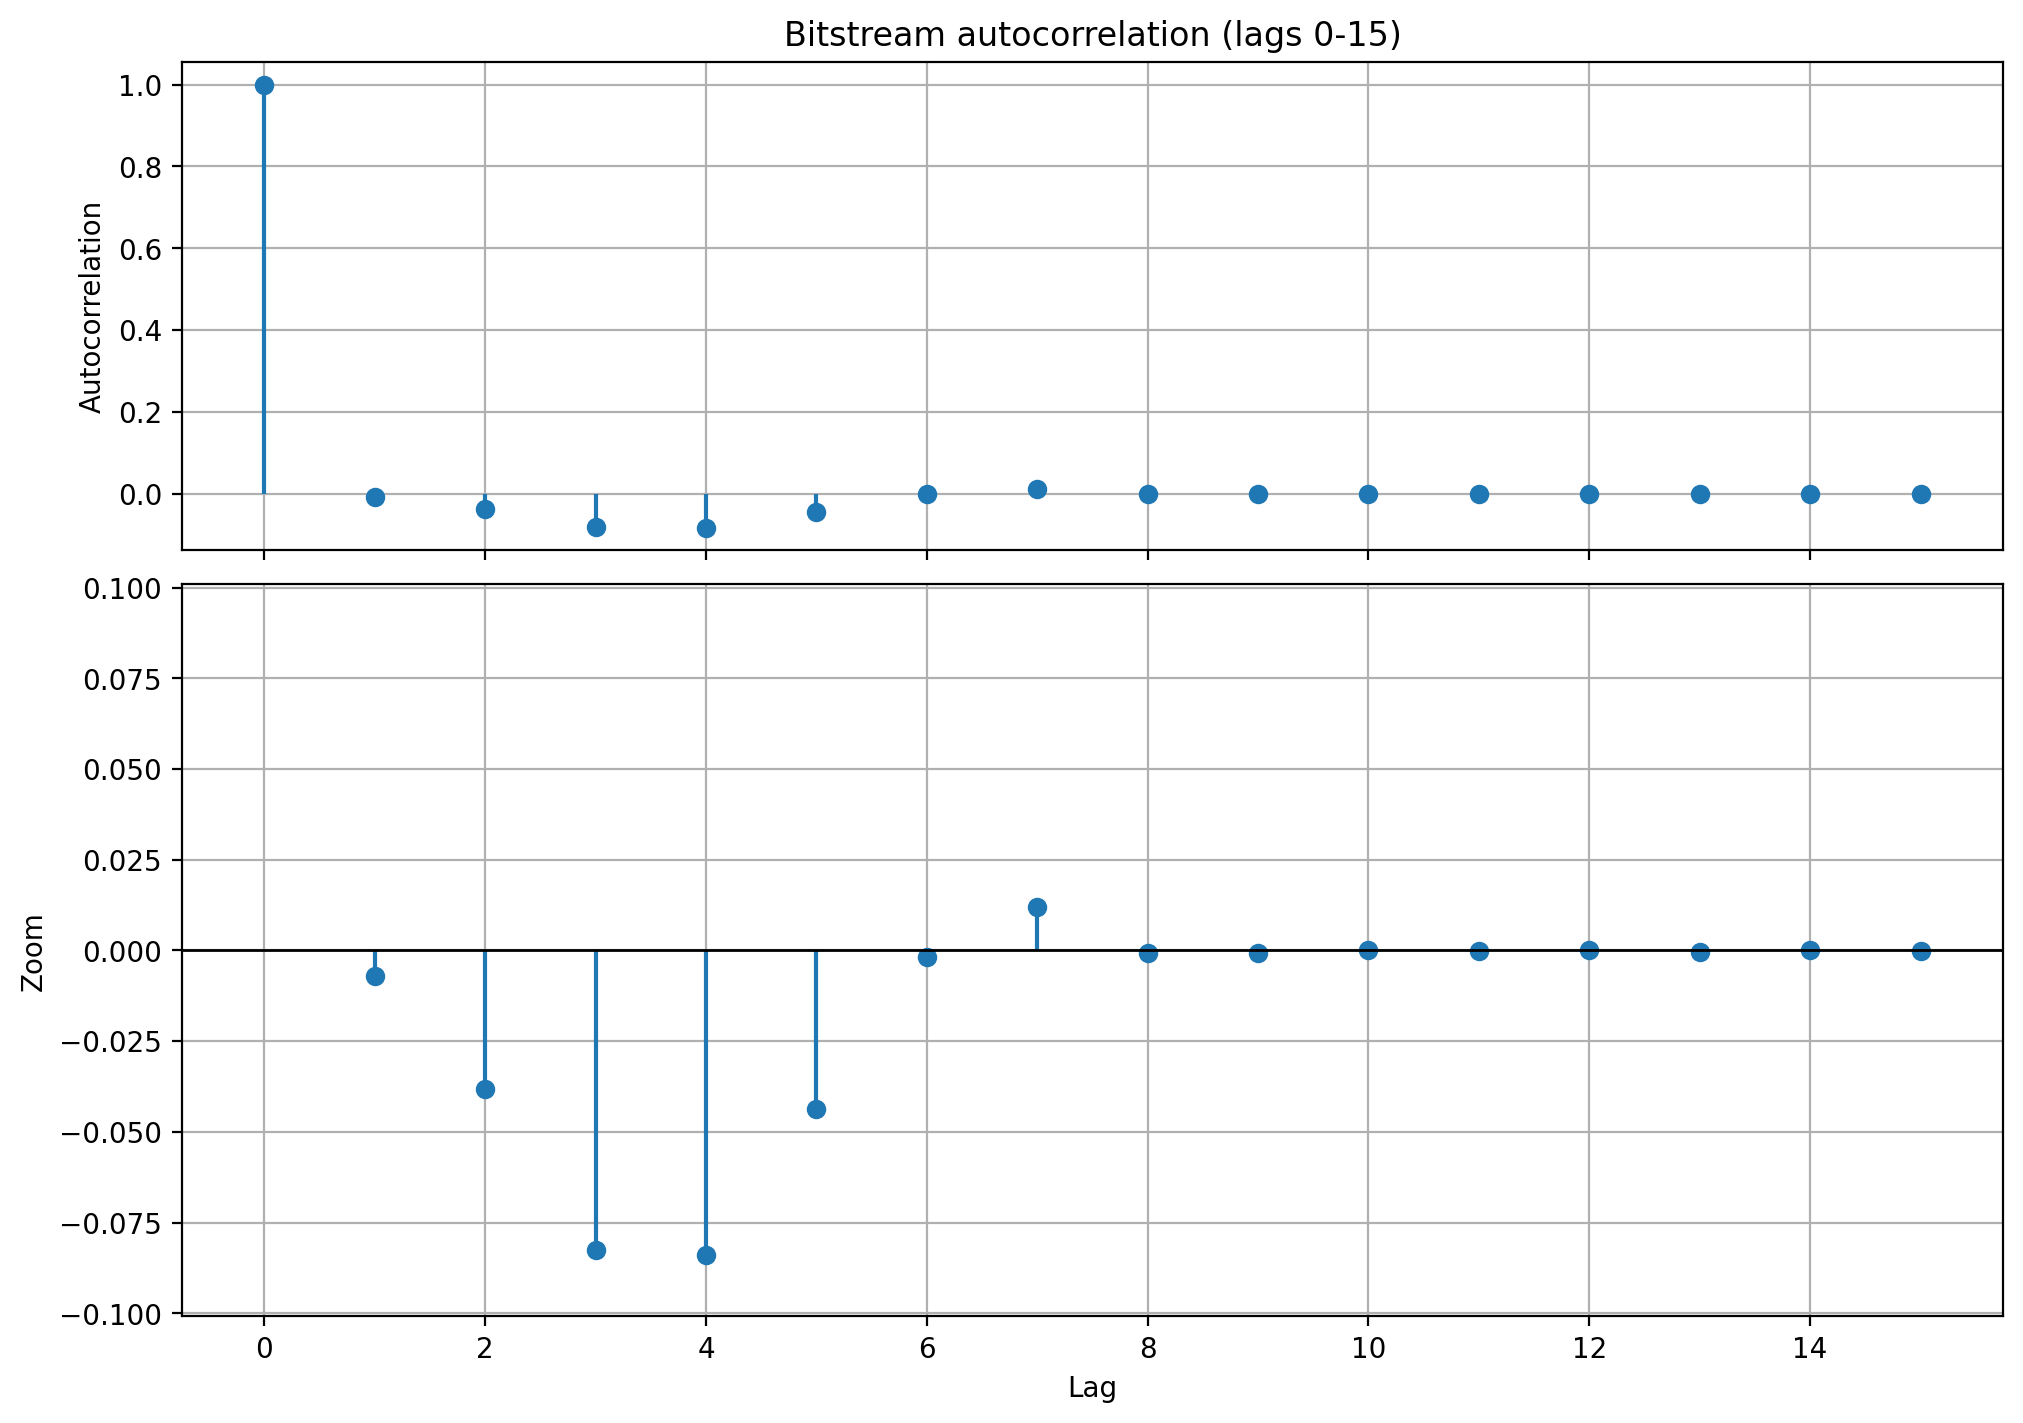
\includegraphics[width=0.9\textwidth]{gfx/spread_ac.png}
    \caption{Autokorelacja strumienia bitów dla oscylatorów rozproszonych w strukturze
    układu, opóźnienia od 0 do 15}
    \label{fig:autokorelacja_rozproszone}
\end{figure}

\begin{table}[htbp]
    \centering
    \caption{Wartości współczynników autokorelacji dla oscylatorów rozproszonych
    w strukturze układu}
    \label{tab:autokorelacja_rozproszone}
    \small
    \begin{tabular}{rrrr}
        \toprule
        Opóźnienie & $R$ & Opóźnienie & $R$ \\
        \midrule
        0 & $+1{,}000000$ & 8  & $-0{,}000588$ \\
        1 & $-0{,}007122$ & 9  & $-0{,}000635$ \\
        2 & $-0{,}038163$ & 10 & $+0{,}000056$ \\
        3 & $-0{,}082474$ & 11 & $-0{,}000165$ \\
        4 & $-0{,}084080$ & 12 & $+0{,}000065$ \\
        5 & $-0{,}043632$ & 13 & $-0{,}000489$ \\
        6 & $-0{,}001822$ & 14 & $+0{,}000223$ \\
        7 & $+0{,}011959$ & 15 & $-0{,}000210$ \\
        \bottomrule
    \end{tabular}
\end{table}

Uzyskany wynik różni się zasadniczo od poprzedniego. W zakresie opóźnień od 1 do 5
występują wyraźnie ujemne współczynniki autokorelacji, osiągające wartość
$-0{,}084080$ dla opóźnienia równego 4. Przy długości serii $N = 10\,485\,760$ bitów
odchylenie standardowe współczynnika dla strumienia w pełni losowego wynosi
$\sigma \approx 3{,}1 \cdot 10^{-4}$, wobec czego zaobserwowana wartość odpowiada
około 270-krotności tego poziomu. Jest to zależność jednoznacznie istotna statystycznie,
a nie efekt naturalnych fluktuacji. Warto zaznaczyć, że wykryte odchylenia mają znak
ujemny, przez co nie mogą być wyjaśnione ewentualną nierównowagą liczby zer i jedynek,
gdyż niezerowa wartość średnia strumienia przesuwałaby współczynniki w kierunku wartości
dodatnich.

Charakter zaobserwowanej zależności wskazuje na skłonność strumienia do naprzemiennej
zmiany wartości bitów w krótkiej skali. Współczynniki narastają w wartości bezwzględnej
od opóźnienia 1 do 4, po czym maleją, a dla opóźnienia 7 przyjmują wartość dodatnią
$+0{,}011959$, co odpowiada blisko 40-krotności odchylenia standardowego. Taki przebieg,
złożony z ujemnego obszaru zakończonego dodatnim maksimum, jest typowy dla strumienia
o częściowo okresowej strukturze, w którym kolejne bity nie są generowane niezależnie,
lecz w powtarzalnym porządku wynikającym z pracy układu ekstrakcji. Ponieważ bity
zapisywane są do bufora w stałej kolejności numerów kanałów, a dla pojedynczego
oscylatora zbocza narastające i opadające występują naprzemiennie, uporządkowanie
oscylatorów według częstotliwości pracy przekłada się bezpośrednio na uporządkowanie
wartości w strumieniu wyjściowym. Zależność ta ma zatem źródło w warstwie serializacji
oraz w relacjach częstotliwości pomiędzy poszczególnymi pierścieniami, a nie w samym
rozproszeniu struktur w obrębie układu.

Dla opóźnień od 8 do 15 wartości współczynników nie przekraczają dwukrotności odchylenia
standardowego i pozostają w granicach naturalnych fluktuacji, co oznacza, że wykryta
zależność ma zasięg ograniczony do kilku najbliższych pozycji i nie prowadzi do
periodyczności w dłuższej skali. Nie odnotowano również wzmocnienia dla opóźnienia
równego 8, obecnego w poprzedniej konfiguracji, co potwierdza, że zmiana rozmieszczenia
oscylatorów wpłynęła na strukturę strumienia, jednak przesunęła obserwowane zależności
w obszar mniejszych opóźnień, zamiast je usunąć.

Wynik ten należy uznać za istotny z punktu widzenia dalszych badań. Pokazuje on, że
poprawa warunków pracy samych źródeł entropii nie jest wystarczająca, jeżeli sposób
łączenia bitów pochodzących z wielu kanałów wprowadza własną, deterministyczną strukturę.
Uzasadnia to konieczność zastosowania etapu korekcji strumienia, którego skuteczność
zbadano w kolejnym podrozdziale, oraz analizy dwuwymiarowych map opóźnień, pozwalającej
ocenić, czy wykryta zależność obejmuje również poziom całych słów.

\FloatBarrier

\subsection{Wyniki pomiaru dla 16 oscylatorów łączonych parami operacją XOR}

W kolejnej konfiguracji liczbę oscylatorów pierścieniowych zwiększono do szesnastu,
przy czym ich wyjścia łączone są parami operacją różnicy symetrycznej, w wyniku czego
do modułu ekstrakcji trafia nadal osiem sygnałów, a przepustowość generatora pozostaje
niezmieniona. Rozmieszczenie struktur w obrębie układu ustalono ręcznie, tak aby
oscylatory tworzące jedną parę znajdowały się w odległych obszarach logiki.

Zastosowanie operacji XOR do łączenia wyjść ma dwie zasadnicze zalety. Po pierwsze,
odchylenie prawdopodobieństwa sygnału wynikowego jest iloczynem odchyleń sygnałów
wejściowych, wobec czego połączenie dwóch niedoskonałych źródeł daje sygnał o rozkładzie
bliższym równomiernemu niż każde z nich osobno. Po drugie, przewidzenie wartości sygnału
wynikowego wymaga znajomości stanu obu oscylatorów jednocześnie, co ogranicza wpływ
okresowego zachowania pojedynczego pierścienia na strumień wyjściowy. Rozdzielenie
przestrzenne oscylatorów tworzących parę jest przy tym warunkiem skuteczności tego
rozwiązania, ponieważ w przypadku struktur położonych blisko siebie wzajemne
oddziaływanie mogłoby prowadzić do ich częściowej synchronizacji, a operacja XOR na dwóch
skorelowanych sygnałach nie wnosi dodatkowej entropii.

Przebieg współczynnika autokorelacji dla omawianej konfiguracji przedstawiono na
rysunku~\ref{fig:autokorelacja_xor}, natomiast dokładne wartości liczbowe zestawiono
w tabeli~\ref{tab:autokorelacja_xor}.

\begin{figure}[htbp]
    \centering
    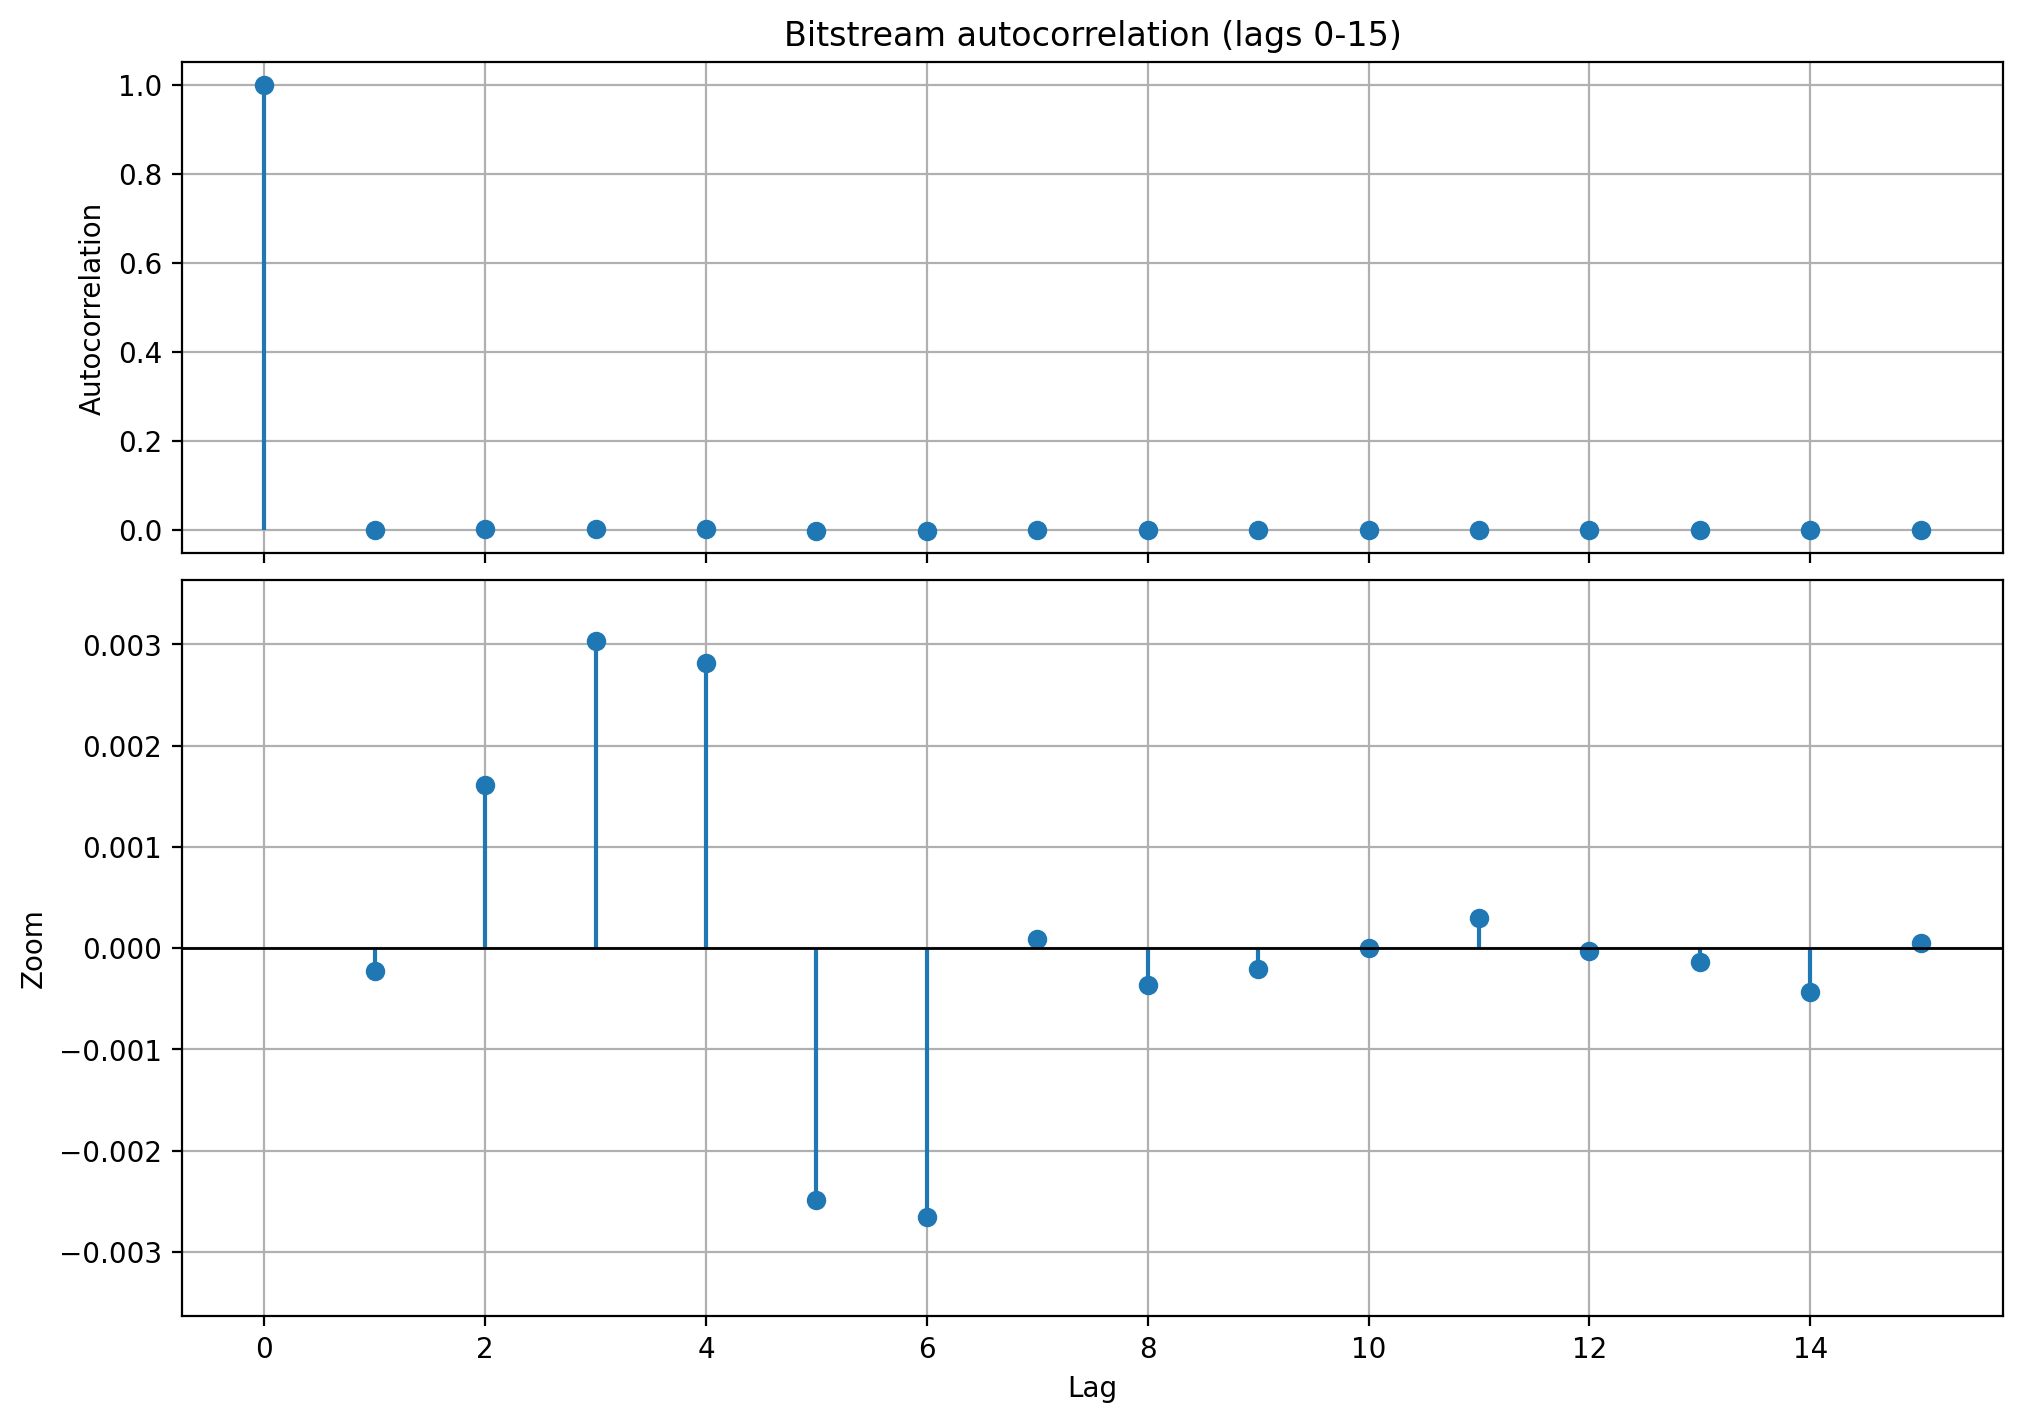
\includegraphics[width=0.9\textwidth]{gfx/xor_ac.png}
    \caption{Autokorelacja strumienia bitów dla 16 oscylatorów łączonych parami operacją
    XOR, opóźnienia od 0 do 15. Zakres dolnego wykresu wynosi $\pm 3 \cdot 10^{-3}$}
    \label{fig:autokorelacja_xor}
\end{figure}

\begin{table}[htbp]
    \centering
    \caption{Wartości współczynników autokorelacji dla 16 oscylatorów łączonych parami
    operacją XOR}
    \label{tab:autokorelacja_xor}
    \small
    \begin{tabular}{rrrr}
        \toprule
        Opóźnienie & $R$ & Opóźnienie & $R$ \\
        \midrule
        0 & $+1{,}000000$ & 8  & $-0{,}000359$ \\
        1 & $-0{,}000221$ & 9  & $-0{,}000207$ \\
        2 & $+0{,}001612$ & 10 & $-0{,}000004$ \\
        3 & $+0{,}003030$ & 11 & $+0{,}000297$ \\
        4 & $+0{,}002819$ & 12 & $-0{,}000024$ \\
        5 & $-0{,}002487$ & 13 & $-0{,}000133$ \\
        6 & $-0{,}002656$ & 14 & $-0{,}000437$ \\
        7 & $+0{,}000093$ & 15 & $+0{,}000047$ \\
        \bottomrule
    \end{tabular}
\end{table}

Zmiana konfiguracji przyniosła wyraźną poprawę w stosunku do poprzedniego pomiaru.
Największa wartość bezwzględna współczynnika dla opóźnień większych od zera wynosi
$0{,}003030$ i występuje dla opóźnienia równego 3, podczas gdy w konfiguracji bez
łączenia wyjść operacją XOR wartość skrajna sięgała $0{,}084080$. Amplituda
zaobserwowanych zależności zmalała zatem blisko dwudziestoośmiokrotnie. Należy przy tym
zwrócić uwagę, że zakres pionowej osi dolnego wykresu na
rysunku~\ref{fig:autokorelacja_xor} jest dobierany automatycznie do zakresu danych
i wynosi w tym przypadku około $\pm 3 \cdot 10^{-3}$, wobec czego bezpośrednie porównanie
wizualne obu rysunków bez uwzględnienia podziałki prowadziłoby do błędnych wniosków.

Wykryte odchylenia pozostają jednak istotne statystycznie. Przy odchyleniu standardowym
$\sigma \approx 3{,}1 \cdot 10^{-4}$ współczynniki dla opóźnień od 2 do 6 odpowiadają
wielokrotnościom tego poziomu w zakresie od pięciu do niemal dziesięciu, co wyklucza
wyjaśnienie ich jako naturalnych fluktuacji. Zmienił się natomiast charakter zależności.
W poprzedniej konfiguracji wszystkie współczynniki w zakresie małych opóźnień były
ujemne, co odpowiadało skłonności do naprzemiennej zmiany wartości bitów. Obecnie
występuje wyraźny podział: dla opóźnień od 2 do 4 współczynniki są dodatnie, natomiast
dla opóźnień 5 i 6 ujemne, przy praktycznym zaniku zależności dla opóźnienia 7
i wszystkich większych. Taki przebieg, obejmujący zwarty obszar zależności dodatnich
przechodzących w ujemne, wskazuje na obecność składowej o okresie rzędu ośmiu pozycji
w strumieniu wyjściowym, a więc odpowiadającej długości pojedynczego bajtu i liczbie
kanałów doprowadzonych do modułu ekstrakcji.

Obserwacja ta potwierdza wniosek sformułowany w poprzednim podrozdziale, zgodnie z którym
zasadnicza część wykrywanych zależności ma źródło w warstwie łączenia bitów pochodzących
z wielu kanałów, a nie w jakości samych źródeł entropii. Podwojenie liczby oscylatorów
oraz łączenie ich wyjść operacją XOR poprawiło właściwości poszczególnych sygnałów
wejściowych, co przełożyło się na znaczną redukcję amplitudy zależności, nie usunęło
jednak deterministycznej struktury wynikającej ze stałej kolejności zapisu kanałów do
bufora. Całkowite wyeliminowanie tego efektu wymagałoby modyfikacji sposobu serializacji
lub zastosowania korekcji strumienia, której skuteczność zbadano w kolejnym podrozdziale.

\FloatBarrier

\subsection{Wyniki pomiaru dla 16 oscylatorów z wybielaniem metodą von Neumanna}

Ostatnia z badanych konfiguracji opiera się na tej samej implementacji sprzętowej co
poprzednia, obejmującej szesnaście oscylatorów pierścieniowych łączonych parami operacją
XOR i rozmieszczonych ręcznie w oddalonych obszarach struktury układu. Różnica dotyczy
wyłącznie przetwarzania po stronie komputera: zarejestrowany strumień poddano wybielaniu
metodą von Neumanna przed wyznaczeniem współczynników autokorelacji.

Analiza tej samej serii pomiarowej w postaci surowej oraz wybielonej pozwala rozdzielić
dwa rodzaje odstępstw od losowości. Metoda von Neumanna usuwa odchylenie
prawdopodobieństwa wystąpienia zera i jedynki, jest natomiast skuteczna wyłącznie przy
założeniu wzajemnej niezależności kolejnych bitów strumienia wejściowego. Odrzucenie par
o jednakowych wartościach zmienia dodatkowo długość i uporządkowanie strumienia, wobec
czego opóźnienia po wybielaniu nie odpowiadają bezpośrednio pozycjom w strumieniu surowym,
a wynikające z tego przesunięcie należy uwzględnić przy porównywaniu obu przebiegów.

Przebieg współczynnika autokorelacji dla strumienia wybielonego przedstawiono na
rysunku~\ref{fig:autokorelacja_vn}, natomiast dokładne wartości liczbowe zestawiono
w tabeli~\ref{tab:autokorelacja_vn}.

\begin{figure}[htbp]
    \centering
    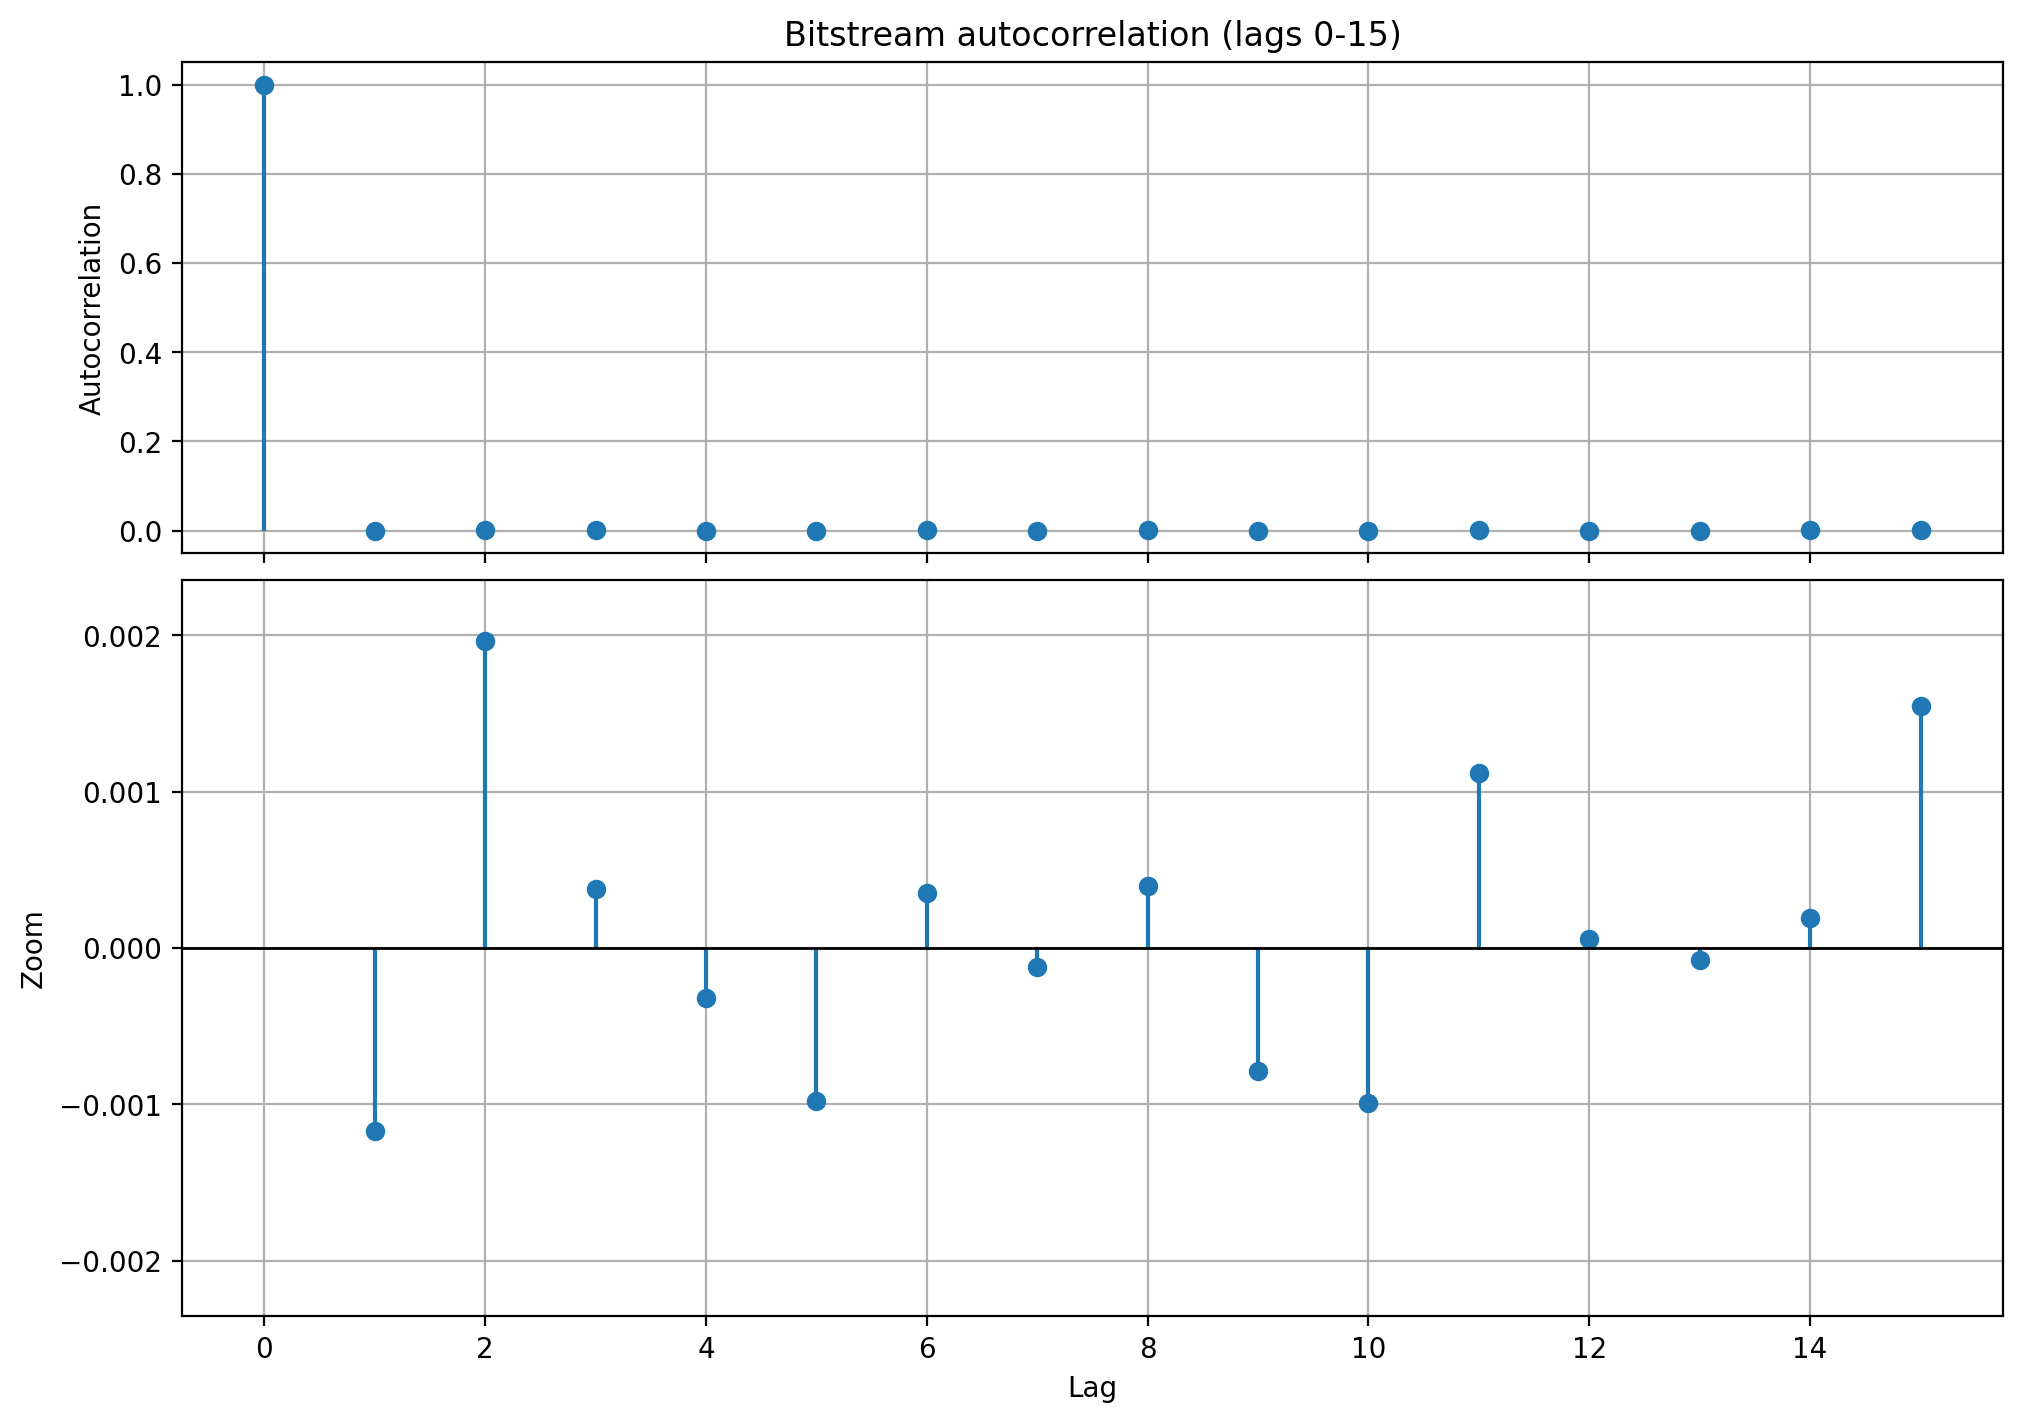
\includegraphics[width=0.9\textwidth]{gfx/vn_ac.png}
    \caption{Autokorelacja strumienia bitów dla 16 oscylatorów łączonych parami operacją
    XOR, po wybielaniu metodą von Neumanna, opóźnienia od 0 do 15. Zakres dolnego wykresu
    wynosi około $\pm 2 \cdot 10^{-3}$}
    \label{fig:autokorelacja_vn}
\end{figure}

\begin{table}[htbp]
    \centering
    \caption{Wartości współczynników autokorelacji dla 16 oscylatorów łączonych parami
    operacją XOR, po wybielaniu metodą von Neumanna}
    \label{tab:autokorelacja_vn}
    \small
    \begin{tabular}{rrrr}
        \toprule
        Opóźnienie & $R$ & Opóźnienie & $R$ \\
        \midrule
        0 & $+1{,}000000$ & 8  & $+0{,}000395$ \\
        1 & $-0{,}001172$ & 9  & $-0{,}000784$ \\
        2 & $+0{,}001963$ & 10 & $-0{,}000990$ \\
        3 & $+0{,}000378$ & 11 & $+0{,}001122$ \\
        4 & $-0{,}000321$ & 12 & $+0{,}000056$ \\
        5 & $-0{,}000977$ & 13 & $-0{,}000079$ \\
        6 & $+0{,}000352$ & 14 & $+0{,}000193$ \\
        7 & $-0{,}000122$ & 15 & $+0{,}001549$ \\
        \bottomrule
    \end{tabular}
\end{table}

Strumień po wybielaniu liczy $2\,620\,032$ bitów, co odpowiada $24{,}99\%$ długości
strumienia wejściowego. Wartość ta jest praktycznie równa teoretycznej granicy jednej
czwartej, osiąganej przez metodę von Neumanna dla źródła o rozkładzie równomiernym.
Sama wydajność wybielania stanowi zatem niezależne potwierdzenie, że strumień wejściowy
nie wykazywał istotnego odchylenia liczby zer i jedynek, ponieważ każde takie odchylenie
prowadziłoby do zwiększenia udziału par odrzucanych i wyraźnie mniejszej długości
wyniku.

Skrócenie serii wymaga skorygowania progu istotności statystycznej. Dla omawianego
strumienia odchylenie standardowe współczynnika autokorelacji przy założeniu pełnej
losowości wynosi $\sigma \approx 6{,}2 \cdot 10^{-4}$, a więc dwukrotnie więcej niż
w poprzednich pomiarach, w których analizowano serie o pełnej długości. Bezpośrednie
porównywanie wartości liczbowych z wcześniejszymi tabelami bez uwzględnienia tej różnicy
byłoby nieuprawnione.

Największą wartość bezwzględną odnotowano dla opóźnienia równego 2, gdzie uzyskano
$R = 0{,}001963$, co odpowiada około 3,2-krotności odchylenia standardowego. Przy
piętnastu jednocześnie badanych opóźnieniach oczekiwana wartość maksymalna dla źródła
losowego mieści się w okolicach trzech odchyleń standardowych, wobec czego zaobserwowany
wynik znajduje się na granicy istotności i nie stanowi sam w sobie dowodu obecności
zależności. Pozostałe współczynniki, w tym $+0{,}001549$ dla opóźnienia 15 oraz
$-0{,}001172$ dla opóźnienia 1, nie przekraczają dwóch i pół odchylenia standardowego.

Istotną zmianą w stosunku do strumienia surowego jest zniknięcie uporządkowanej struktury
obejmującej opóźnienia od 2 do 6. W pomiarze bez wybielania współczynniki w tym zakresie
tworzyły zwarty obszar wartości dodatnich przechodzących w ujemne, przy czym każda z nich
przekraczała pięciokrotność odchylenia standardowego. Po wybielaniu znaki współczynników
w całym badanym zakresie rozkładają się nieregularnie, a ich wartości nie tworzą
rozpoznawalnego wzorca, co odpowiada obrazowi oczekiwanemu dla strumienia bez zależności
lokalnych. Należy przy tym pamiętać, że odrzucanie par o jednakowych wartościach
przekształca skalę opóźnień, wobec czego zależność występująca w strumieniu surowym na
określonej pozycji nie zostałaby po wybielaniu odwzorowana na tej samej pozycji, lecz
rozmyta w otoczeniu proporcjonalnym do stopnia redukcji długości. Sam brak struktury
w przebiegu po wybielaniu nie jest zatem równoważny stwierdzeniu, że mechanizm
odpowiedzialny za jej powstanie przestał działać w warstwie sprzętowej.

Zestawienie wyników wszystkich czterech badanych konfiguracji, wraz z odniesieniem do
pozostałych zastosowanych metod analizy statystycznej, przedstawiono w~podrozdziale
podsumowującym.

\FloatBarrier

\section{Analiza utworzonych słów bitowych za pomocą map 2D}

Mapy dwuwymiarowe zastosowano w celu oceny właściwości statystycznych słów utworzonych z badanego 
strumienia bitów oraz analizy zależności pomiędzy słowami oddalonymi od siebie o zadane opóźnienie. 
Dla każdej rozpatrywanej konfiguracji wyznaczano pary w postaci $(w[n],\,w[n+\tau])$, gdzie $w[n]$ 
oznacza bieżące słowo bitowe, natomiast $w[n+\tau]$ słowo przesunięte o opóźnienie $\tau$. 
Następnie ilość wystąpień poszczególnych par przedstawiano w postaci histogramu dwuwymiarowego.

W przypadku generatora o dobrych właściwościach losowych rozkład punktów na mapie 2D powinien być 
możliwie jednorodny, bez wyraźnych struktur geometrycznych, pasów oraz nadmiernej koncentracji 
zliczeń w określonych obszarach. 
Pojawienie się pasów pionowych lub poziomych wskazuje, że niektóre wartości słów występują 
częściej od innych, co świadczy o nierównomierności rozkładu. 
Z kolei zwiększona koncentracja punktów w pobliżu przekątnej może sugerować istnienie zależności 
pomiędzy kolejnymi słowami, a więc obecność korelacji czasowej w analizowanym ciągu.

\FloatBarrier

\subsection{Mapy dla 8 oscylatorów rozmieszczonych automatycznie}

Analizę map dwuwymiarowych rozpoczęto od konfiguracji podstawowej, w~której oscylatory
zostały rozmieszczone automatycznie przez narzędzie implementacyjne. Mapy dla słów
czterobitowych przedstawiono na rysunku~\ref{fig:map2d_auto_w4}.

\begin{figure}[ht]
    \centering
    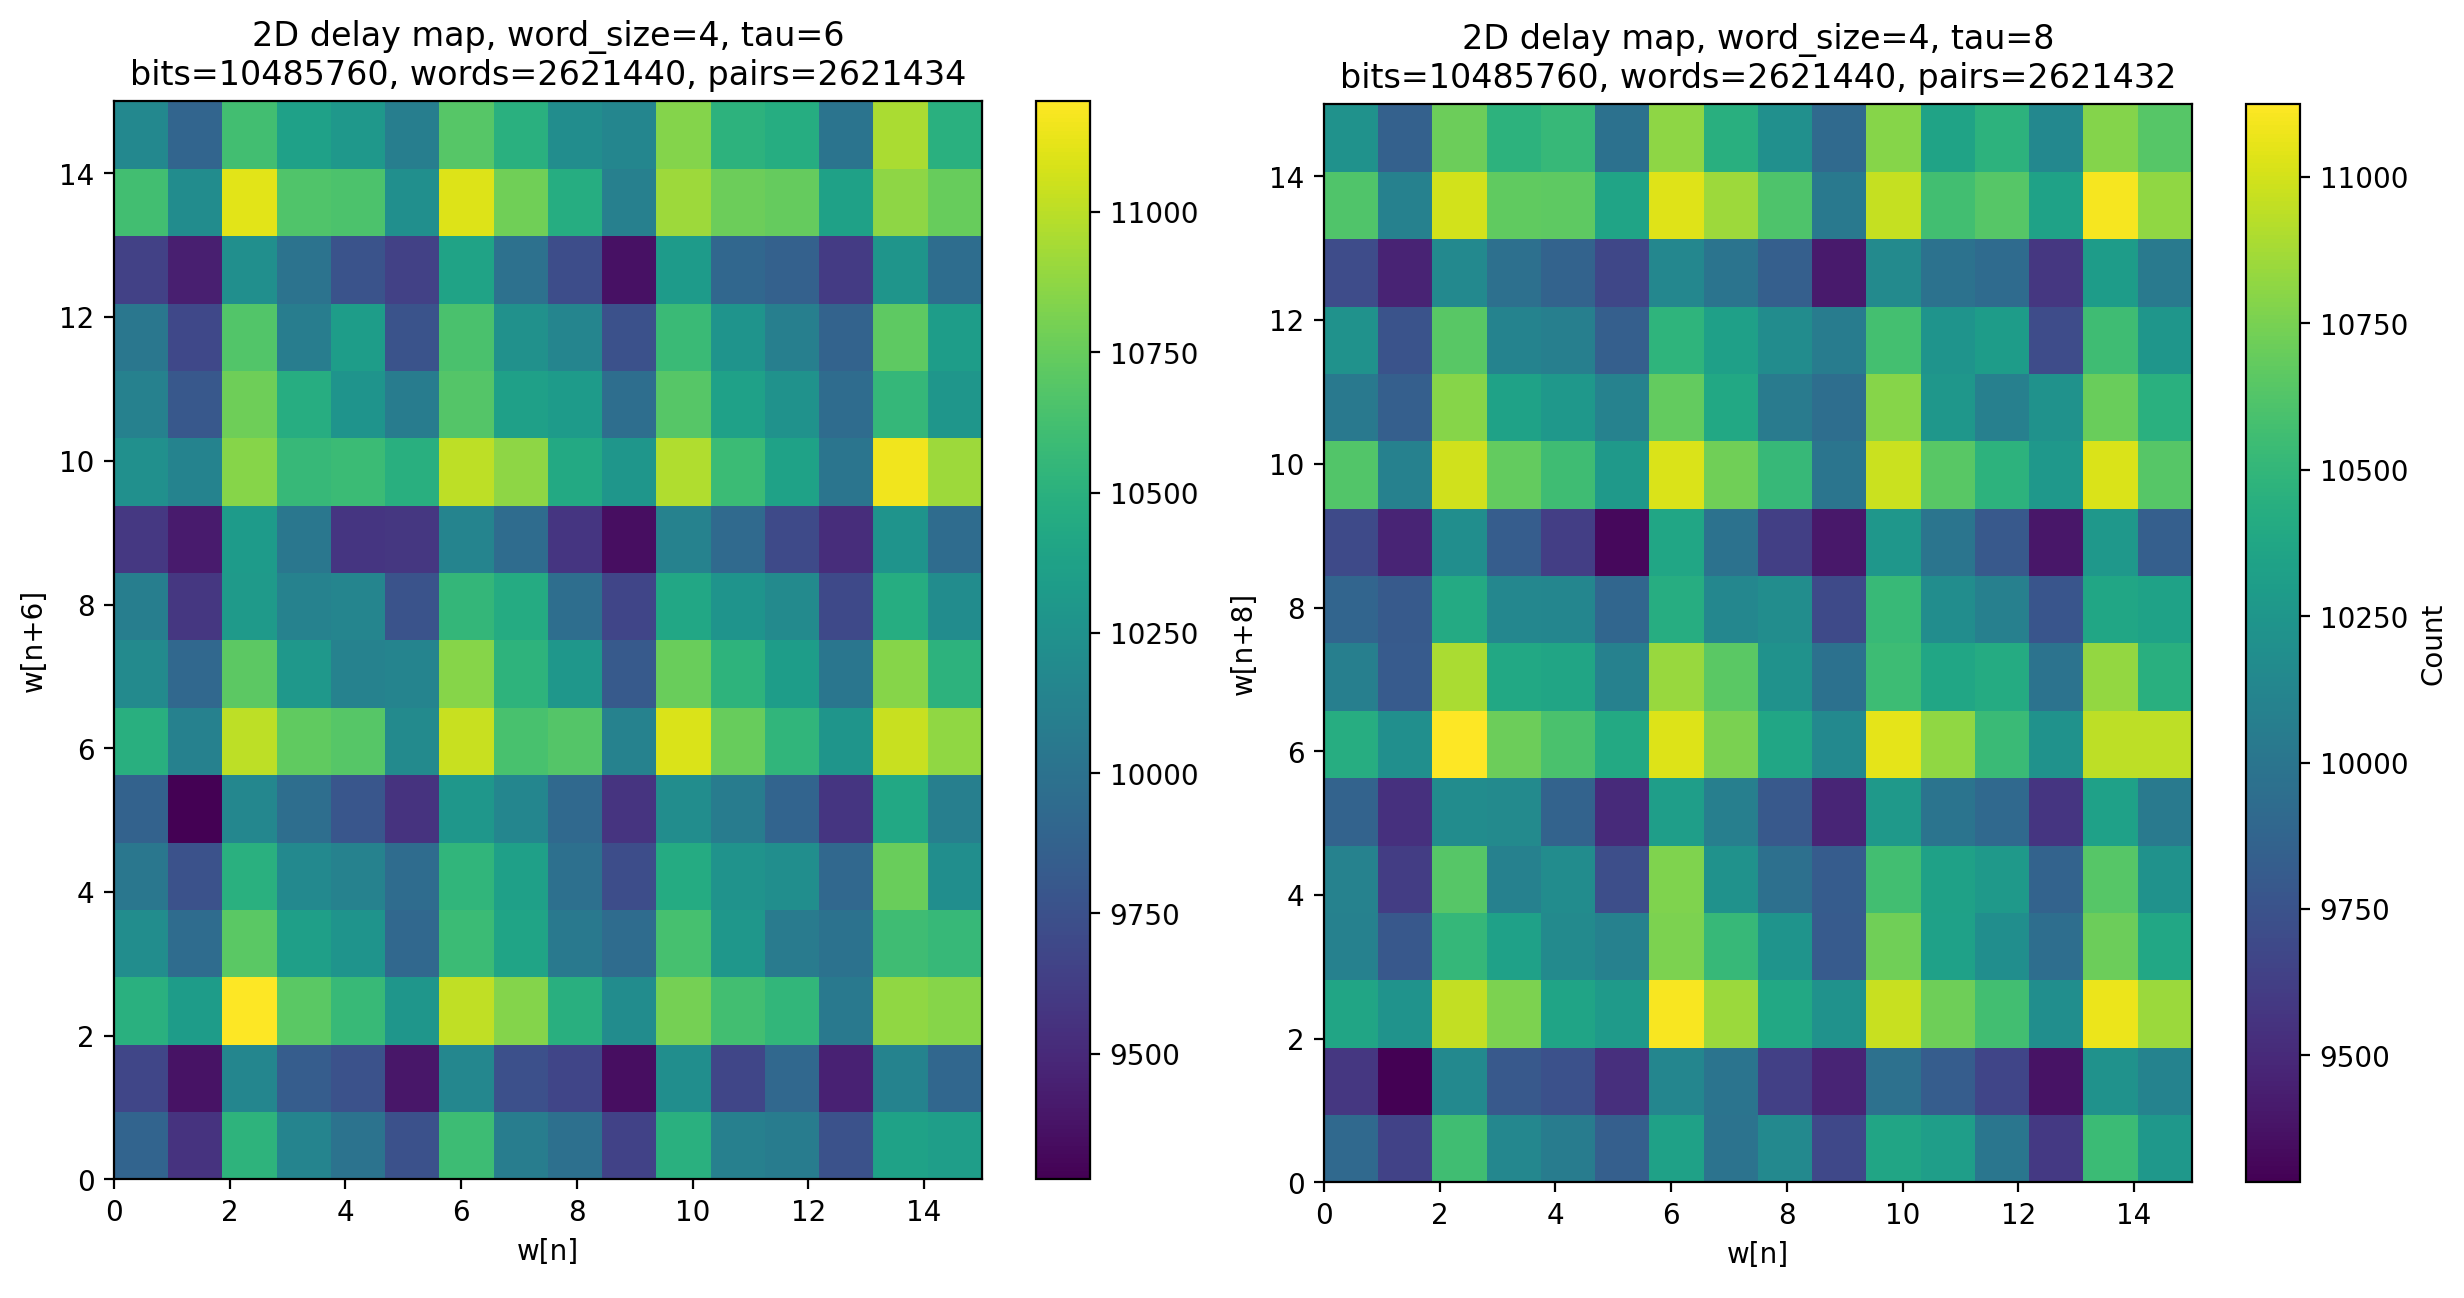
\includegraphics[width=0.98\textwidth]{gfx/no_wh_2d_w4_t6_t8}
    \caption{Mapy 2D dla 8 oscylatorów rozmieszczonych automatycznie, przy parametrach
    $word\_size = 4$ oraz $\tau = 6$, $\tau = 8$.}
    \label{fig:map2d_auto_w4}
\end{figure}

Dla słów czterobitowych widoczny jest regularny układ jaśniejszych i~ciemniejszych pasów,
biegnących zarówno poziomo, jak i~pionowo. Podwyższone zliczenia występują dla wartości
słów o~numerach $2$, $6$, $10$ oraz $14$, natomiast obniżone dla wartości $1$, $5$, $9$
i~$13$. Wszystkie wyróżnione wartości mają wspólną cechę: różnią się o~cztery, a~więc
odpowiadają jednakowemu stanowi dwóch najmłodszych bitów przy zmiennych bitach starszych.
Wskazuje to, że nierównomierność dotyczy przede wszystkim określonych pozycji w~obrębie
słowa, a~zatem konkretnych kanałów wejściowych, nie zaś wartości słowa jako całości.

Przy $2\,621\,434$ analizowanych parach i~$256$ komórkach histogramu wartość oczekiwana
zliczenia wynosi $10\,240$, a~odpowiadające jej odchylenie standardowe rozkładu Poissona
około $101$ zliczeń. Odnotowany zakres, obejmujący przedział od około $9\,400$ do
$11\,100$, odpowiada zatem odchyleniu skrajnemu na poziomie $8{,}5$ odchylenia
standardowego. Rozkład wartości słów odbiega więc od równomiernego w~sposób jednoznacznie
istotny statystycznie, choć skala tego odstępstwa jest znacznie mniejsza niż stwierdzona
później dla konfiguracji z~ręcznym rozmieszczeniem oscylatorów.

Struktura pasowa jest praktycznie identyczna dla obu badanych opóźnień, co oznacza, że
wynika ona z~rozkładu prawdopodobieństwa pojedynczych słów, a~nie z~zależności pomiędzy
słowami oddalonymi w~strumieniu. Mapa dwuwymiarowa jest w~tym przypadku w~przybliżeniu
iloczynem dwóch identycznych rozkładów brzegowych, co odpowiada wzajemnej niezależności
obu współrzędnych przy jednoczesnym odstępstwie każdej z~nich od rozkładu równomiernego.
Nie zaobserwowano również podwyższonych zliczeń wzdłuż przekątnej, a~więc powtarzalność
całych słów po zadanym opóźnieniu nie występuje.

\begin{figure}[ht]
    \centering
    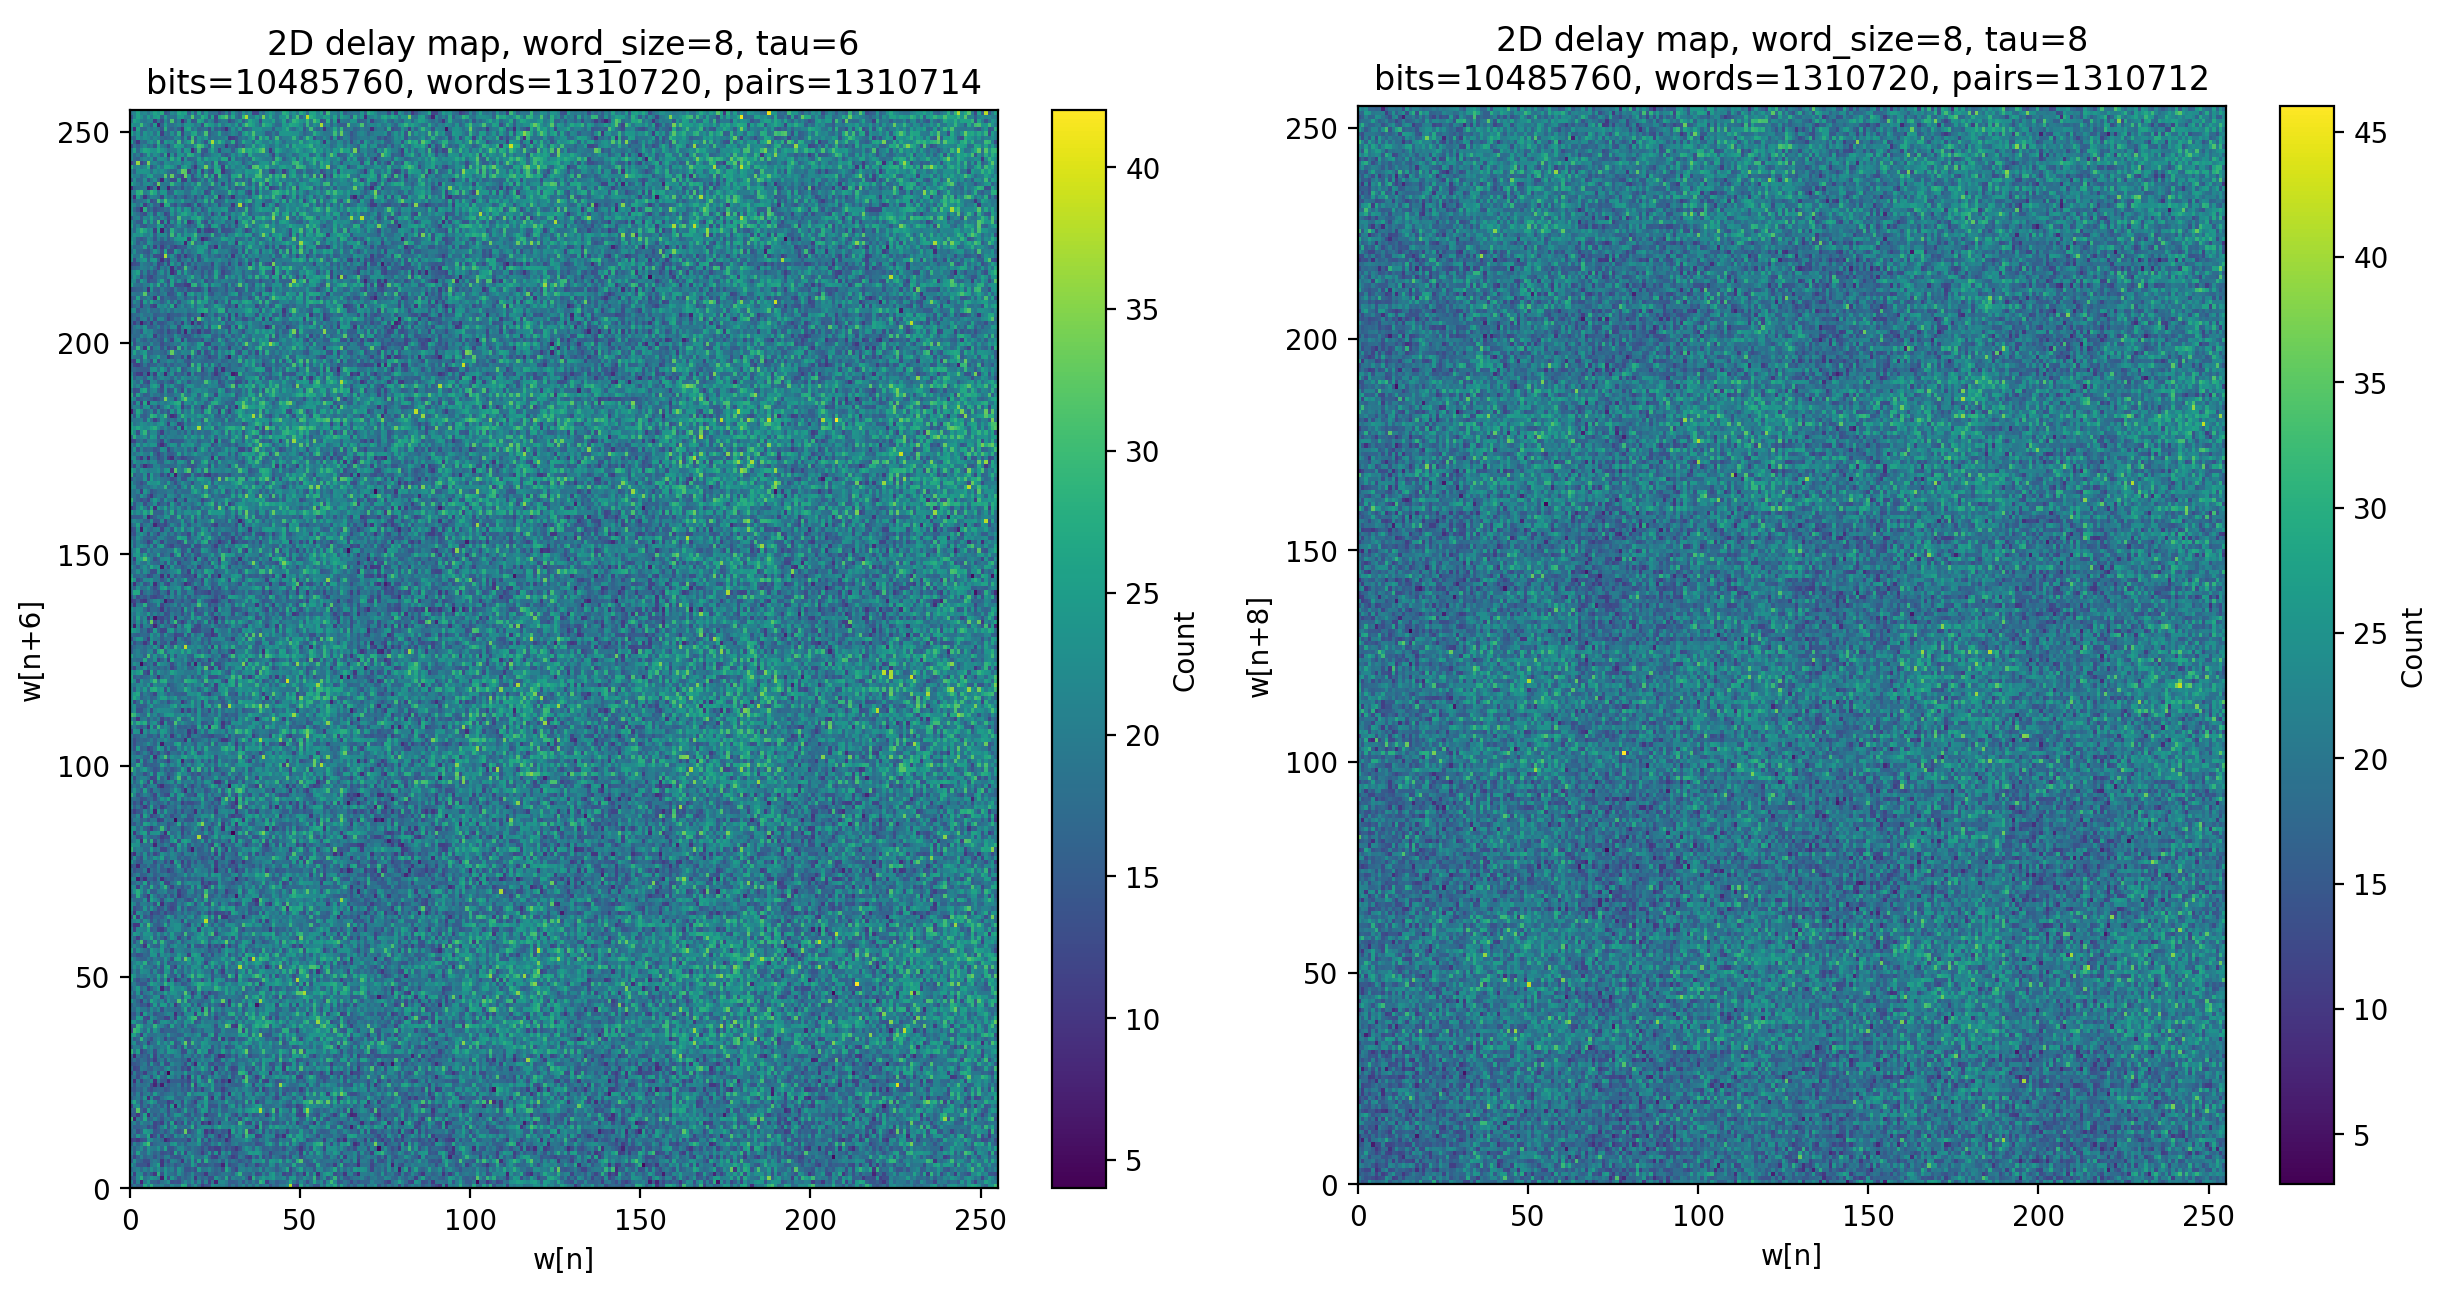
\includegraphics[width=0.98\textwidth]{gfx/no_wh_2d_w8_t6_t8}
    \caption{Mapy 2D dla 8 oscylatorów rozmieszczonych automatycznie, przy parametrach
    $word\_size = 8$ oraz $\tau = 6$, $\tau = 8$.}
    \label{fig:map2d_auto_w8}
\end{figure}

Mapy dla słów ośmiobitowych, przedstawione na rysunku~\ref{fig:map2d_auto_w8}, mają
charakter drobnoziarnistego szumu, w~którym regularna struktura widoczna dla słów
czterobitowych przestaje być rozpoznawalna. Wynika to z~liczności: przy $1\,310\,714$
parach rozłożonych na $65\,536$ komórek wartość oczekiwana zliczenia wynosi zaledwie
dwadzieścia, a~odpowiadające jej odchylenie standardowe około cztery i~pół. Odnotowany
zakres od trzech do czterdziestu sześciu zliczeń odpowiada odchyleniu skrajnemu rzędu
pięciu do sześciu odchyleń standardowych, jednak przy tak dużej liczbie komórek
rozpatrywanych jednocześnie wystąpienie takich wartości jest oczekiwane dla źródła
losowego. Mapa ta potwierdza zatem jedynie brak struktur wielkoskalowych i~nie pozwala
na ilościową ocenę rozkładu, a~za miarodajne dla tej konfiguracji przyjęto wyniki
uzyskane dla słów czterobitowych.

Zestawienie tego wyniku z~testem odchylenia rozkładu prowadzi do obserwacji wartej
podkreślenia. Dla omawianej konfiguracji test monobitowy wykazał odchylenie na poziomie
jedenastu odchyleń standardowych, a~mapy dwuwymiarowe rozrzut zliczeń na poziomie
ośmiu i~pół. Obie metody wskazują zatem zgodnie na istotne odstępstwo od losowości,
przy czym mapy dodatkowo lokalizują je: nierównomierność dotyczy wybranych pozycji
bitowych w~obrębie słowa, co odpowiada zróżnicowaniu właściwości poszczególnych
kanałów wejściowych, a~nie jednolitemu przesunięciu całego strumienia.

\FloatBarrier

\subsection{Mapy dla 8 oscylatorów rozproszonych w strukturze układu}

W konfiguracji z oscylatorami rozmieszczonymi ręcznie w oddalonych obszarach struktury
mapy dwuwymiarowe zachowują ogólny charakter obrazu uzyskanego poprzednio, ujawniają
jednak wyraźniejszą strukturę wewnętrzną. Mapy dla słów czterobitowych przedstawiono na
rysunku~\ref{fig:map2d_spread_w4}.

\begin{figure}[ht]
    \centering
    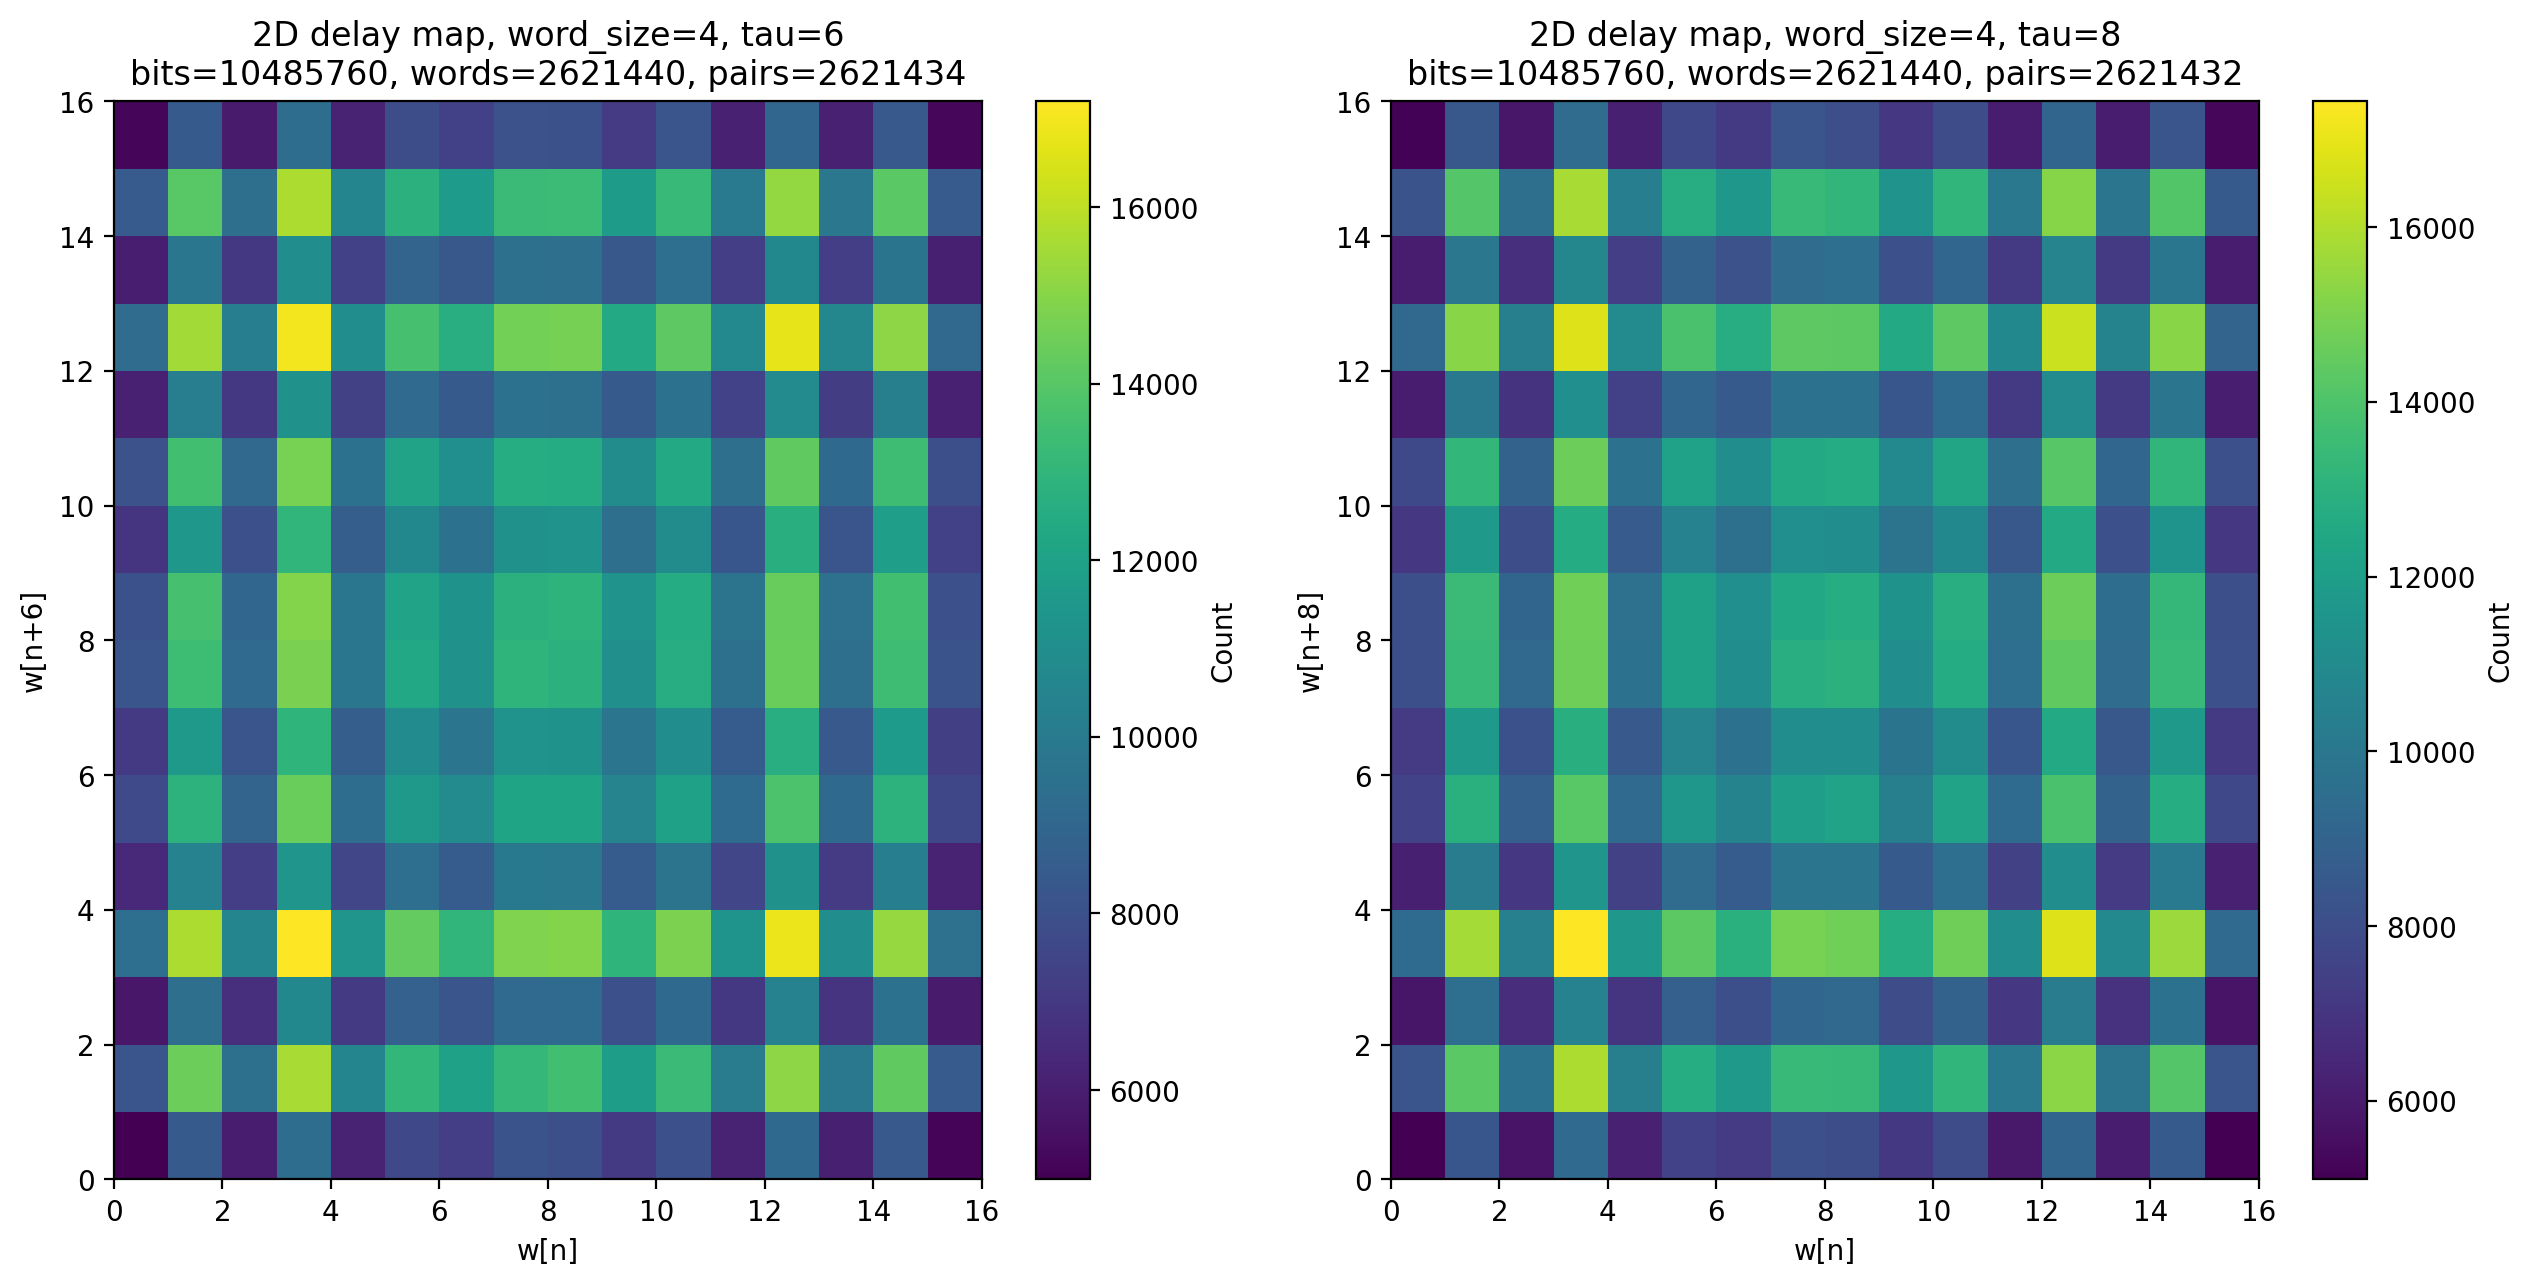
\includegraphics[width=0.70\textwidth]{gfx/spread_2d_w4_t6_t8}
    \caption{Mapy 2D dla oscylatorów rozproszonych w strukturze układu, przy parametrach
    $word\_size = 4$ oraz $\tau = 6$, $\tau = 8$.}
    \label{fig:map2d_spread_w4}
\end{figure}

Dla słów czterobitowych widoczny jest regularny układ jaśniejszych i ciemniejszych pasów
biegnących zarówno poziomo, jak i pionowo. Rozkład ten nie jest przypadkowy: podwyższone
zliczenia występują dla wartości słów o numerach 3, 12 oraz sąsiadujących z nimi,
natomiast wyraźnie obniżone dla wartości skrajnych, to jest 0 i 15. Odpowiada to
odpowiednio kombinacjom bitów o naprzemiennej strukturze oraz kombinacjom złożonym
z bitów jednakowych. Obraz ten stanowi bezpośrednie potwierdzenie wniosku sformułowanego
przy analizie autokorelacji, gdzie dla tej konfiguracji odnotowano silne ujemne
współczynniki w zakresie małych opóźnień: skłonność strumienia do naprzemiennej zmiany
wartości bitów przekłada się na uprzywilejowanie tych wartości słów, w których bity
sąsiednie się różnią, oraz na rzadsze występowanie słów o bitach jednakowych.
Zestawienie map dla dwóch różnych opóźnień pozwala rozdzielić dwa efekty. Struktura pasowa
jest praktycznie identyczna dla $\tau = 6$ i $\tau = 8$, co oznacza, że wynika ona z
rozkładu prawdopodobieństwa pojedynczych słów, a nie z zależności pomiędzy słowami
oddalonymi o zadane opóźnienie. Mapa dwuwymiarowa jest w tym przypadku w przybliżeniu
iloczynem dwóch identycznych rozkładów brzegowych, co odpowiada wzajemnej niezależności
obu współrzędnych przy jednoczesnym odstępstwie każdej z nich od rozkładu równomiernego.

\begin{figure}[ht]
    \centering
    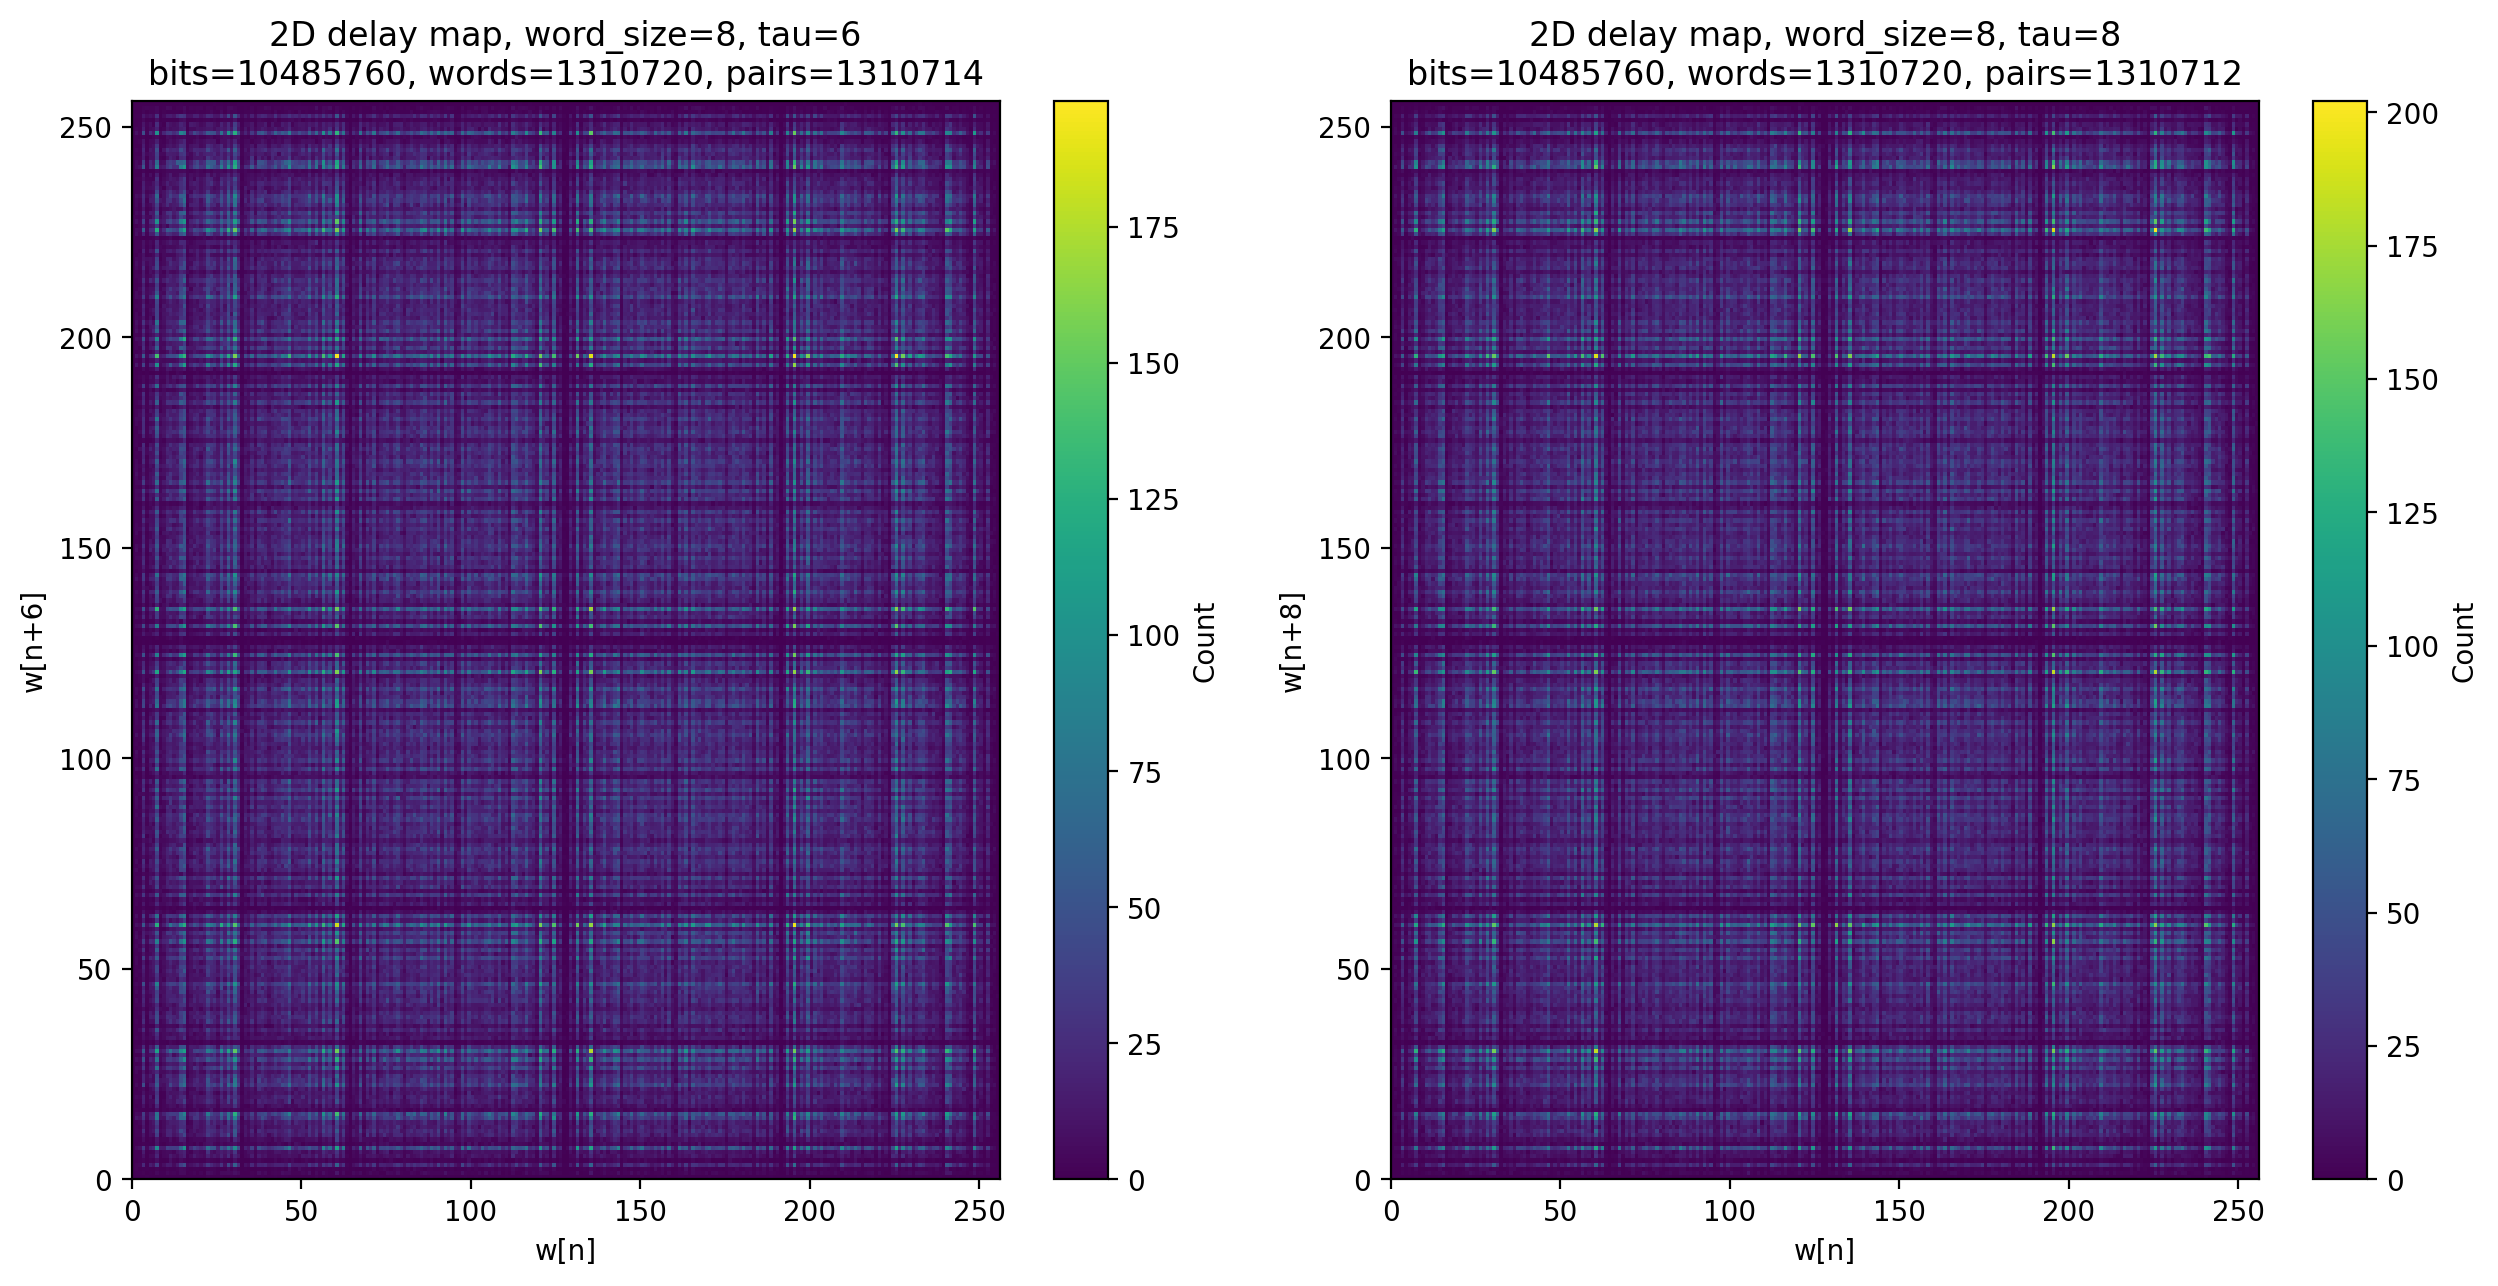
\includegraphics[width=0.98\textwidth]{gfx/spread_2d_w8_t6_t8}
    \caption{Mapy 2D dla oscylatorów rozproszonych w strukturze układu, przy parametrach
    $word\_size = 8$ oraz $\tau = 6$, $\tau = 8$.}
    \label{fig:map2d_spread_w8}
\end{figure}

Mapy dla słów ośmiobitowych, przedstawione na rysunku~\ref{fig:map2d_spread_w8},
ujawniają tę samą prawidłowość w bardziej rozbudowanej postaci. Widoczna jest regularna
siatka linii o obniżonych zliczeniach, dzieląca obszar mapy na bloki o rozmiarze
odpowiadającym w przybliżeniu 32 oraz 64 jednostkom, a więc potęgom liczby dwa. Położenie
tych linii wskazuje na uprzywilejowanie określonych bitów w obrębie bajtu, co jest
oczekiwane wobec faktu, że kolejne pozycje bajtu wypełniane są bitami pochodzącymi od
różnych oscylatorów, pracujących z różnymi częstotliwościami. Nie odnotowano natomiast
podwyższonych zliczeń wzdłuż przekątnej, co potwierdza, że powtarzalność całych bajtów
po zadanym opóźnieniu nie występuje.

Porównanie z konfiguracją poprzednią prowadzi do wniosku, że ręczne rozmieszczenie
oscylatorów nie usunęło nierównomierności rozkładu wartości słów, lecz uczyniło ją
wyraźniejszą. Jest to spójne z wynikiem badania autokorelacji dla tej konfiguracji
i wskazuje, że źródłem obserwowanego efektu nie są warunki pracy poszczególnych
pierścieni, a sposób łączenia bitów pochodzących z wielu kanałów w bajty wyjściowe.

\FloatBarrier

\subsection{Mapy dla 16 oscylatorów łączonych parami operacją XOR}

W konfiguracji obejmującej szesnaście oscylatorów, których wyjścia łączone są parami
operacją XOR, obraz map dwuwymiarowych zmienia się zasadniczo. Mapy dla słów
czterobitowych przedstawiono na rysunku~\ref{fig:map2d_xor_w4}.

\begin{figure}[ht]
    \centering
    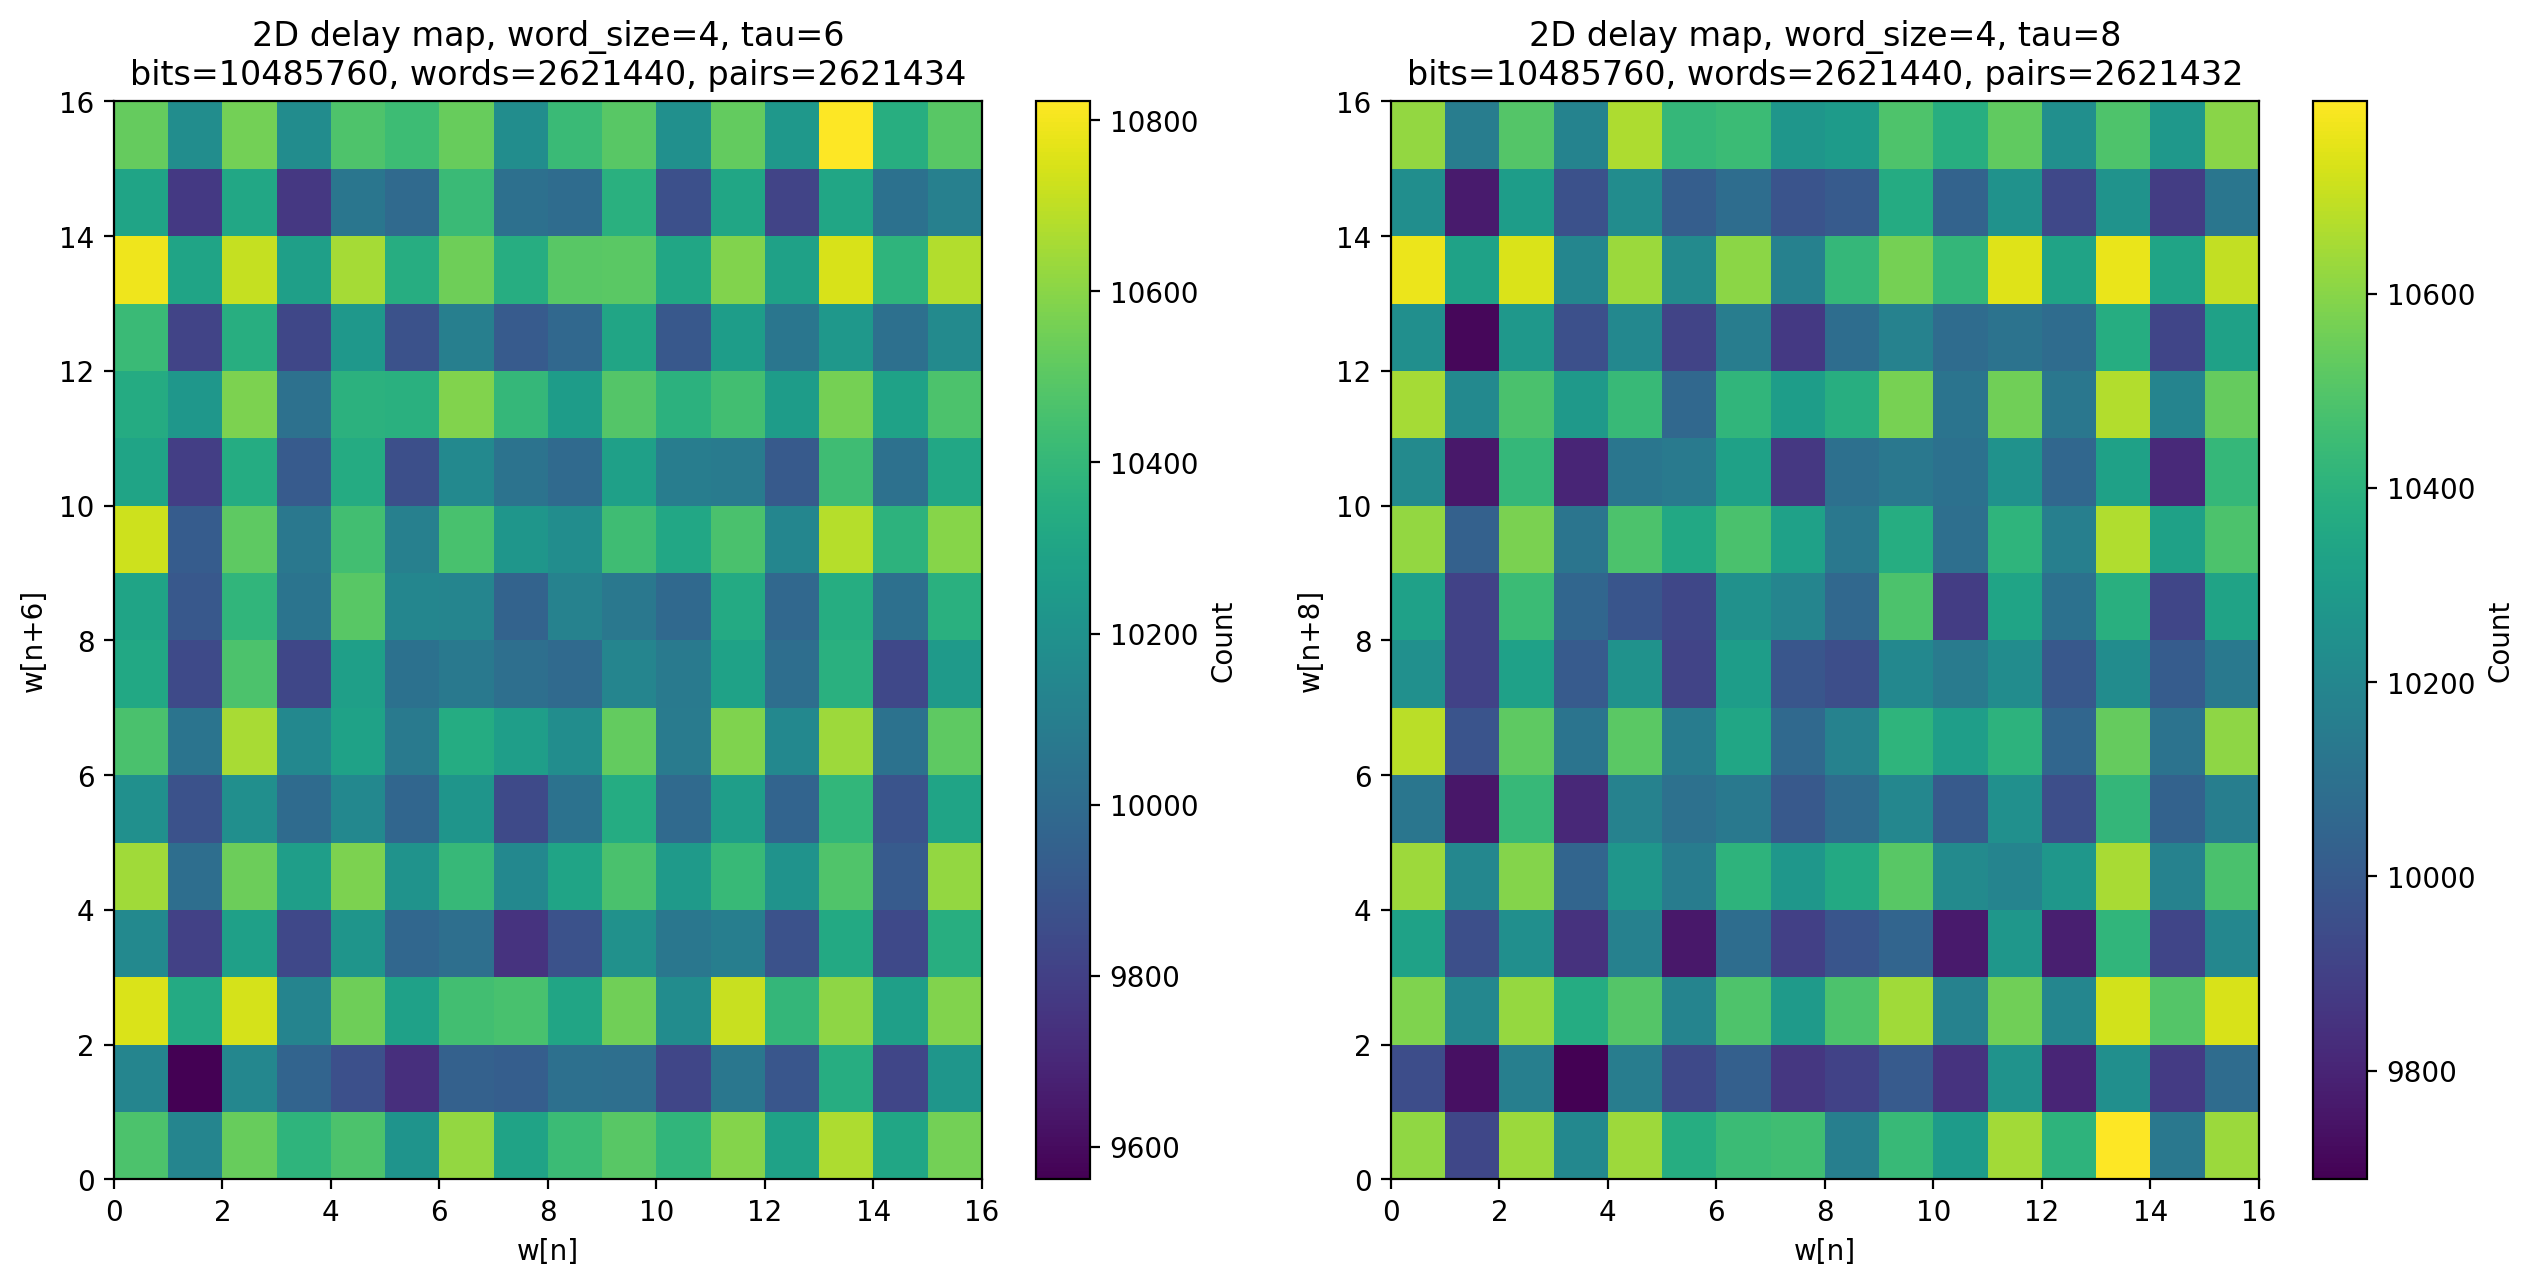
\includegraphics[width=0.98\textwidth]{gfx/xor_2d_w4_t6_t8}
    \caption{Mapy 2D dla 16 oscylatorów łączonych parami operacją XOR, przy parametrach
    $word\_size = 4$ oraz $\tau = 6$, $\tau = 8$.}
    \label{fig:map2d_xor_w4}
\end{figure}

Regularna struktura pasowa, dominująca w poprzednich konfiguracjach, przestała być
widoczna. Zliczenia rozkładają się nieregularnie w całym obszarze mapy, bez
uprzywilejowania określonych wartości słów. Zasadnicza zmiana dotyczy jednak nie samego
układu jasnych i ciemnych komórek, lecz zakresu skali barwnej. Dla konfiguracji bez
łączenia operacją XOR zliczenia obejmowały przedział od około $5\,500$ do $17\,000$,
natomiast obecnie mieszczą się w przedziale od $9\,600$ do $10\,800$. Przy $2\,621\,434$
analizowanych parach i $256$ komórkach histogramu wartość oczekiwana wynosi około
$10\,240$ zliczeń, wobec czego odnotowane odchylenia nie przekraczają sześciu procent
tej wielkości, gdy poprzednio sięgały ponad sześćdziesięciu procent. Interpretacja map
wymaga zatem każdorazowego odczytania zakresu skali, ponieważ jest on dobierany
automatycznie do zawartości danych i mapa o silnym kontraście wizualnym może
przedstawiać rozkład bliższy równomiernemu niż mapa pozornie jednorodna.

Dla źródła w pełni losowego zliczenia w komórkach podlegają rozkładowi Poissona,
którego odchylenie standardowe jest równe pierwiastkowi z wartości oczekiwanej i wynosi
w tym przypadku około $101$ zliczeń. Zaobserwowany rozrzut, obejmujący przedział około
$\pm 600$ zliczeń wokół wartości średniej, odpowiada zatem blisko sześciu odchyleniom
standardowym, co oznacza, że rozkład wartości słów nadal odbiega od równomiernego,
choć skala tego odstępstwa zmalała o rząd wielkości.

\begin{figure}[ht]
    \centering
    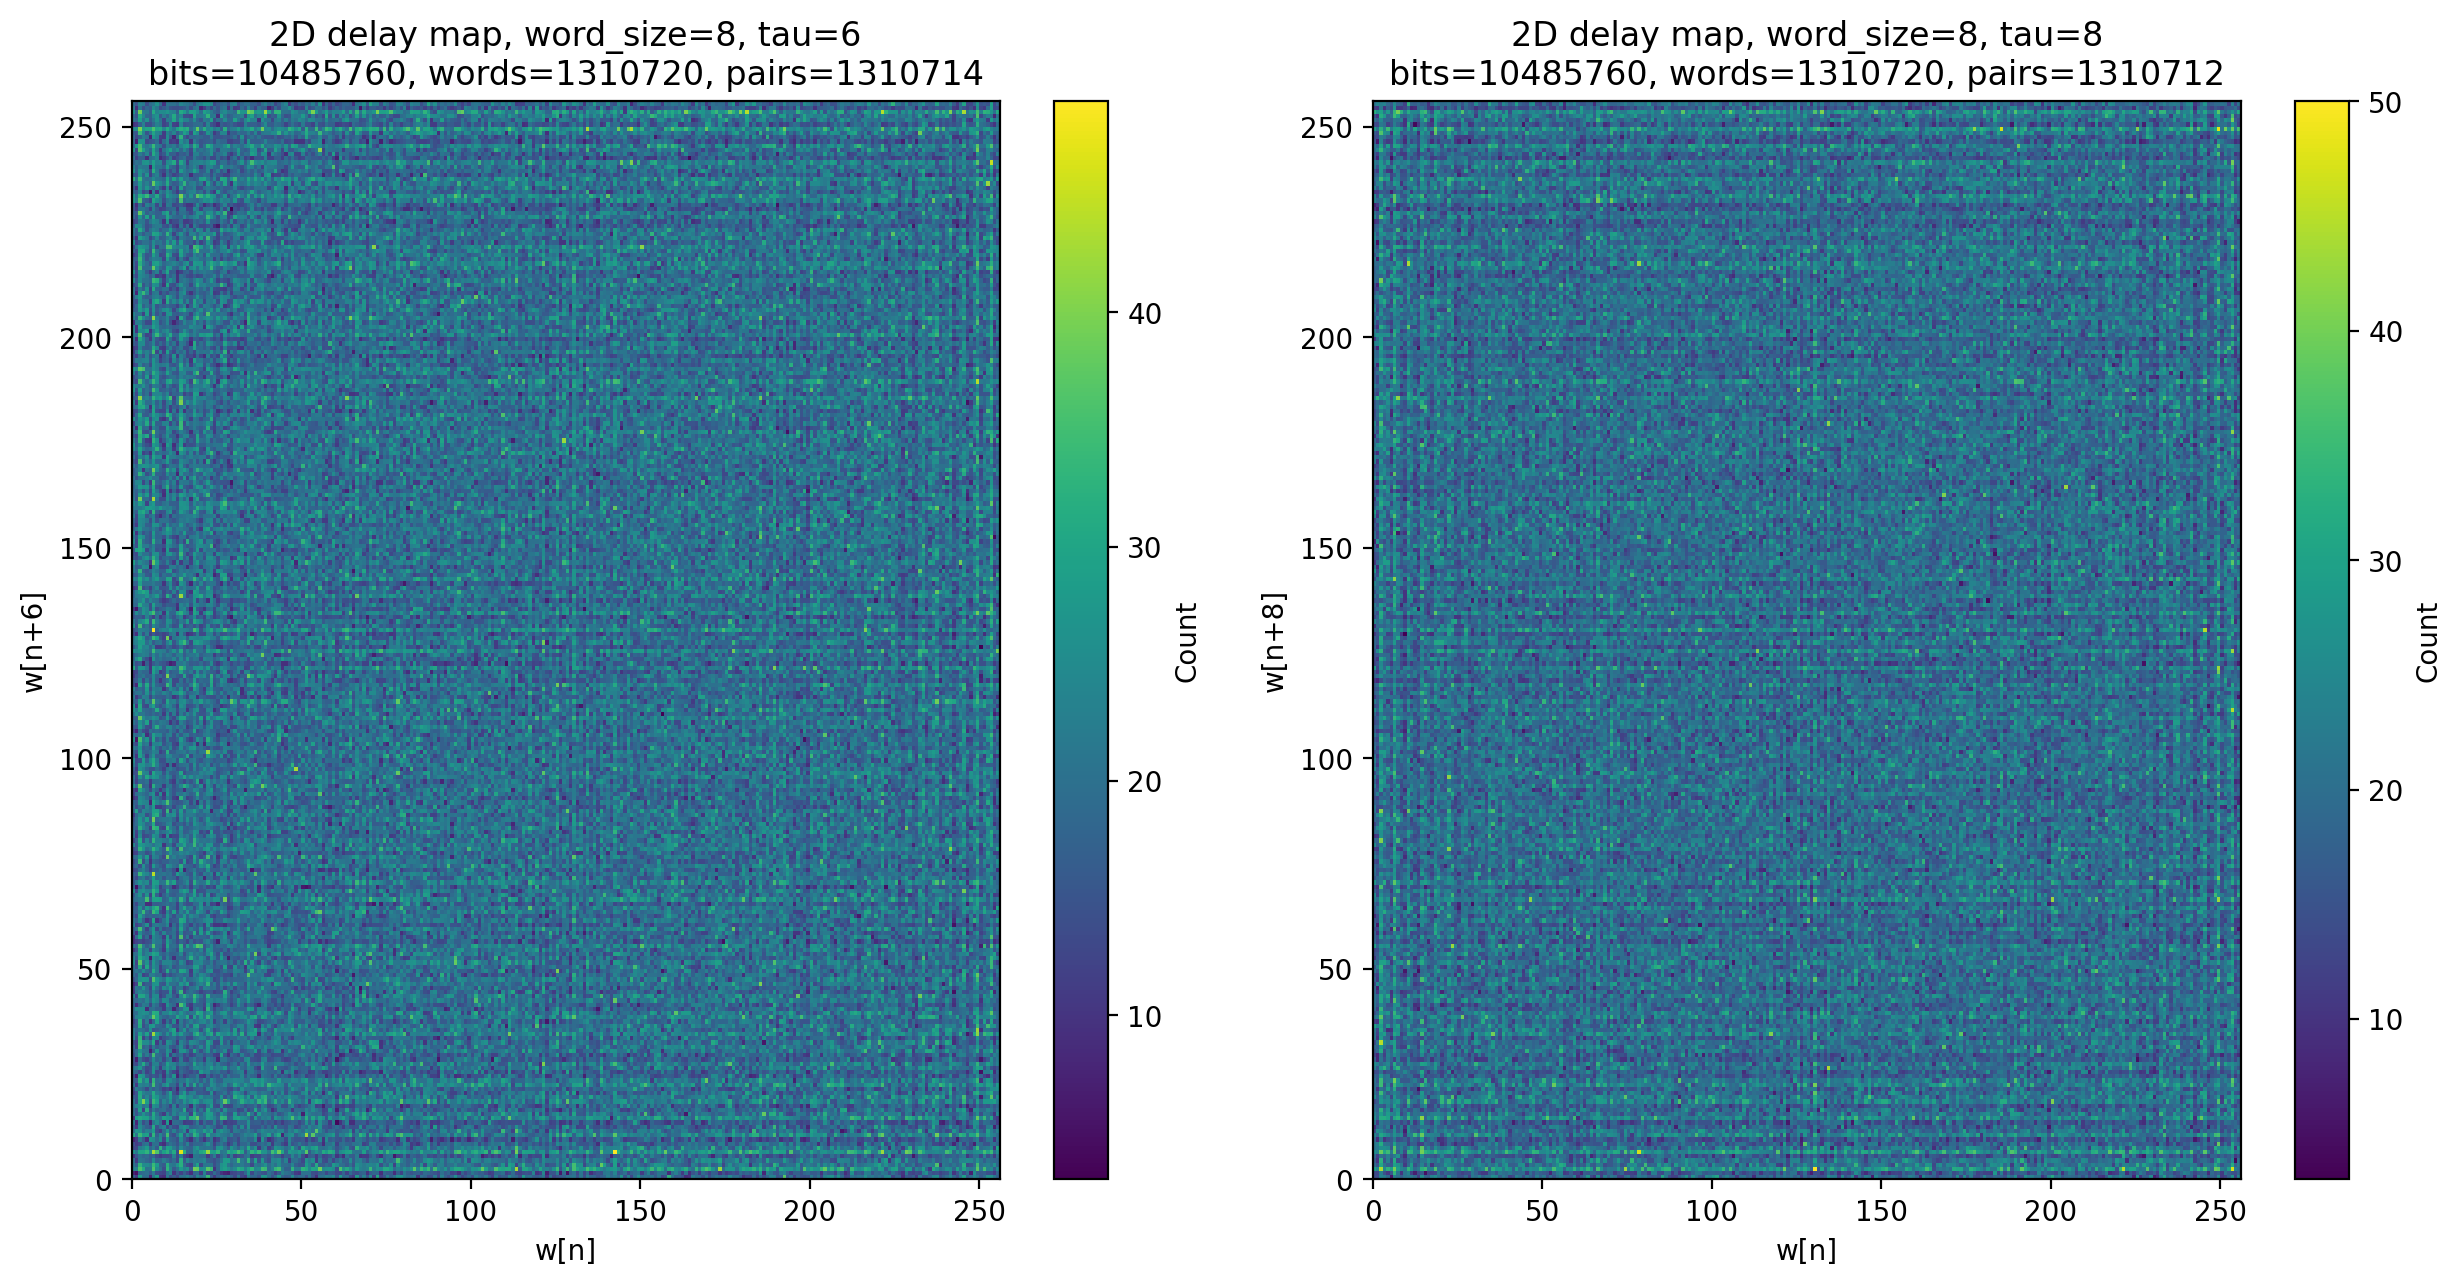
\includegraphics[width=0.98\textwidth]{gfx/xor_2d_w8_t6_t8}
    \caption{Mapy 2D dla 16 oscylatorów łączonych parami operacją XOR, przy parametrach
    $word\_size = 8$ oraz $\tau = 6$, $\tau = 8$.}
    \label{fig:map2d_xor_w8}
\end{figure}

Mapy dla słów ośmiobitowych, przedstawione na rysunku~\ref{fig:map2d_xor_w8}, mają
charakter drobnoziarnistego szumu, bez widocznej siatki linii o obniżonych zliczeniach,
obecnej w konfiguracjach poprzednich. Pewne pozostałości struktury dają się dostrzec
w postaci nieznacznie jaśniejszych pasm przy krawędziach obszaru, odpowiadających
wartościom bajtów o skrajnie małych i skrajnie dużych numerach. Przy $1\,310\,712$
parach rozłożonych na $65\,536$ komórek wartość oczekiwana zliczenia wynosi jedynie
około dwudziestu, a odpowiadające jej odchylenie standardowe około czterech i pół,
wobec czego znaczna część widocznego kontrastu jest naturalnym rozrzutem statystycznym,
nie zaś cechą generatora. Przy tak małej liczbie zliczeń na komórkę mapa dla słów
ośmiobitowych traci wartość diagnostyczną i pełni funkcję głównie jakościową,
potwierdzając brak wyraźnych struktur wielkoskalowych.

W żadnej z przedstawionych map nie występują podwyższone zliczenia wzdłuż przekątnej,
co oznacza brak skłonności do powtarzania tej samej wartości słowa po zadanym
opóźnieniu. Porównanie map dla $\tau = 6$ oraz $\tau = 8$ nie ujawnia istotnych różnic,
z czego wynika, że pozostałe odstępstwa od rozkładu równomiernego dotyczą
prawdopodobieństw wystąpienia poszczególnych wartości słów, a nie zależności pomiędzy
słowami oddalonymi w strumieniu.

\FloatBarrier

\subsection{Mapy dla 16 oscylatorów z wybielaniem metodą von Neumanna}

Ostatnią analizę wykonano dla tej samej serii pomiarowej co poprzednio, poddanej
wybielaniu metodą von Neumanna. Skrócenie strumienia do $2\,620\,032$ bitów zmniejsza
liczbę analizowanych par, a tym samym wartość oczekiwaną zliczenia w komórce histogramu,
co należy uwzględnić przy porównywaniu zakresów skali barwnej z mapami wcześniejszymi.
Mapy dla słów czterobitowych przedstawiono na rysunku~\ref{fig:map2d_vn_w4}.

\begin{figure}[ht]
    \centering
    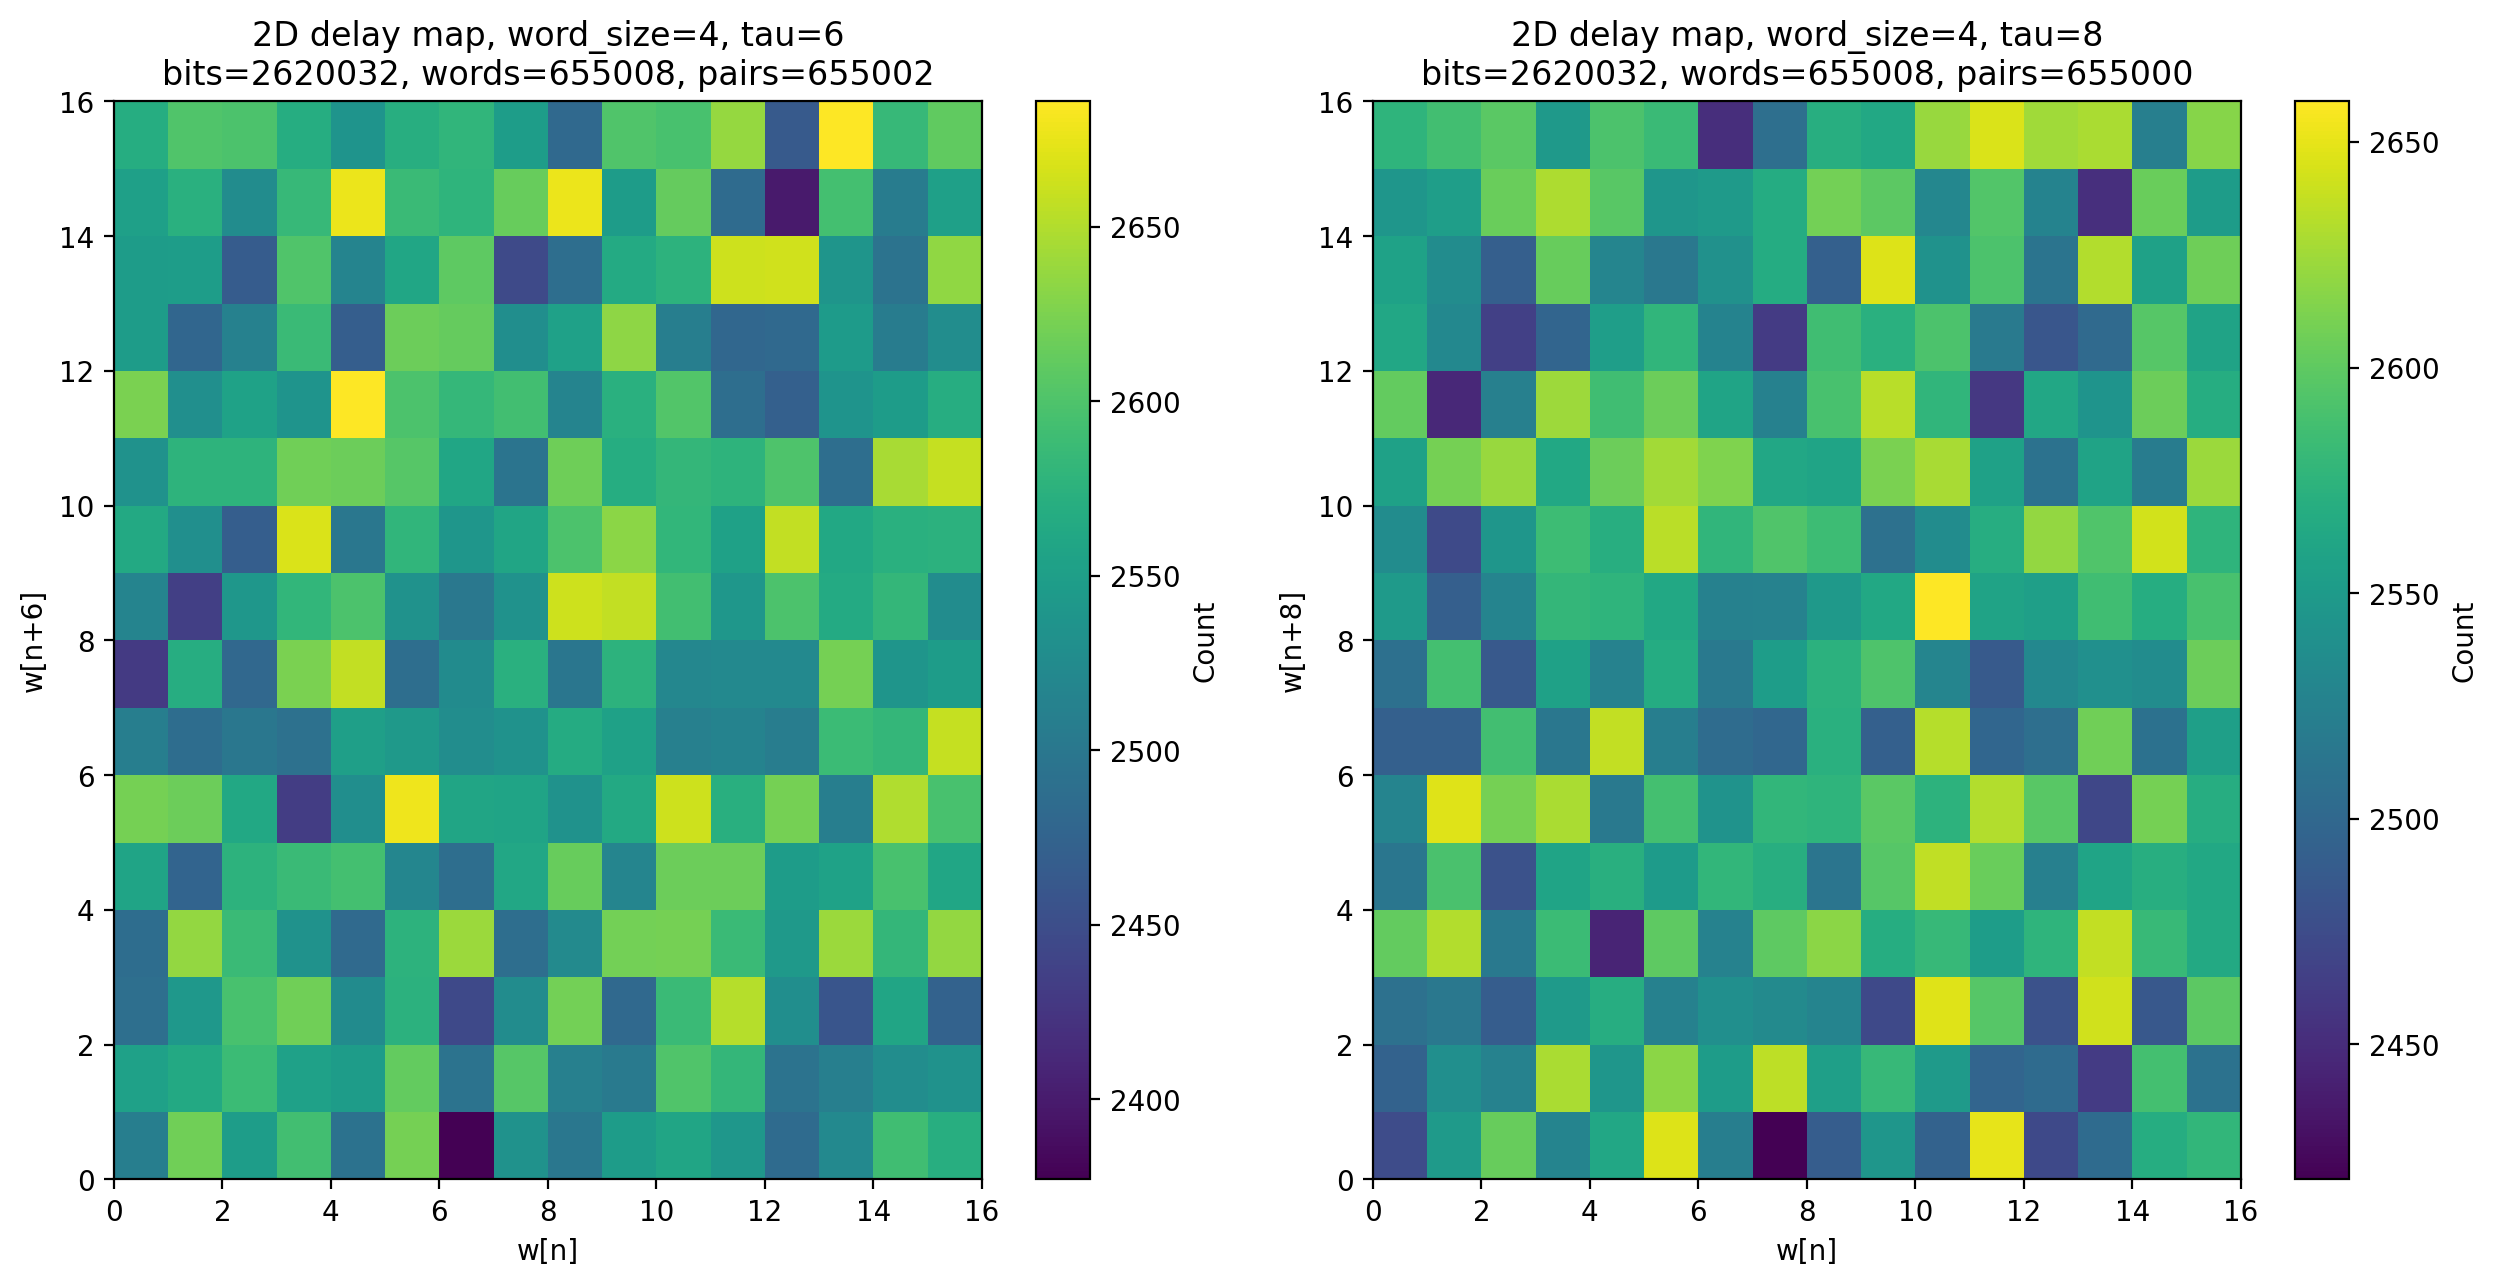
\includegraphics[width=0.98\textwidth]{gfx/vn_2d_w4_t6_t8}
    \caption{Mapy 2D dla 16 oscylatorów łączonych parami operacją XOR, po wybielaniu
    metodą von Neumanna, przy parametrach $word\_size = 4$ oraz $\tau = 6$, $\tau = 8$.}
    \label{fig:map2d_vn_w4}
\end{figure}

Dla słów czterobitowych liczba par wynosi $655\,002$, co przy $256$ komórkach histogramu
daje wartość oczekiwaną około $2\,559$ zliczeń oraz odpowiadające jej odchylenie
standardowe rozkładu Poissona równe około $51$ zliczeniom. Odnotowany zakres zliczeń,
obejmujący przedział od około $2\,390$ do $2\,680$, odpowiada zatem odchyleniu skrajnemu
na poziomie $3{,}3$ odchylenia standardowego dla $\tau = 6$ oraz $2{,}7$ dla $\tau = 8$.
Jest to wynik istotnie lepszy od uzyskanego dla strumienia surowego, w którym odchylenie
skrajne sięgało blisko sześciu odchyleń standardowych. Przy $256$ jednocześnie
analizowanych komórkach wartość maksymalna rzędu trzech odchyleń standardowych jest
zgodna z oczekiwaniem dla rozkładu równomiernego, wobec czego dla tej długości słowa nie
stwierdzono istotnego odstępstwa od losowości.

Porównanie z konfiguracją bez wybielania prowadzi do wniosku, że resztkowa
nierównomierność rozkładu wartości słów, obserwowana w strumieniu surowym, wynikała
w znacznej części z odchylenia prawdopodobieństwa pojedynczych bitów, a nie z zależności
strukturalnych. Metoda von Neumanna, usuwając odchylenie rozkładu, zredukowała je do
poziomu naturalnych fluktuacji statystycznych. Jest to spójne z wynikiem analizy
autokorelacji dla tej konfiguracji, gdzie po wybielaniu również nastąpił zanik
uporządkowanej struktury współczynników.

\begin{figure}[ht]
    \centering
    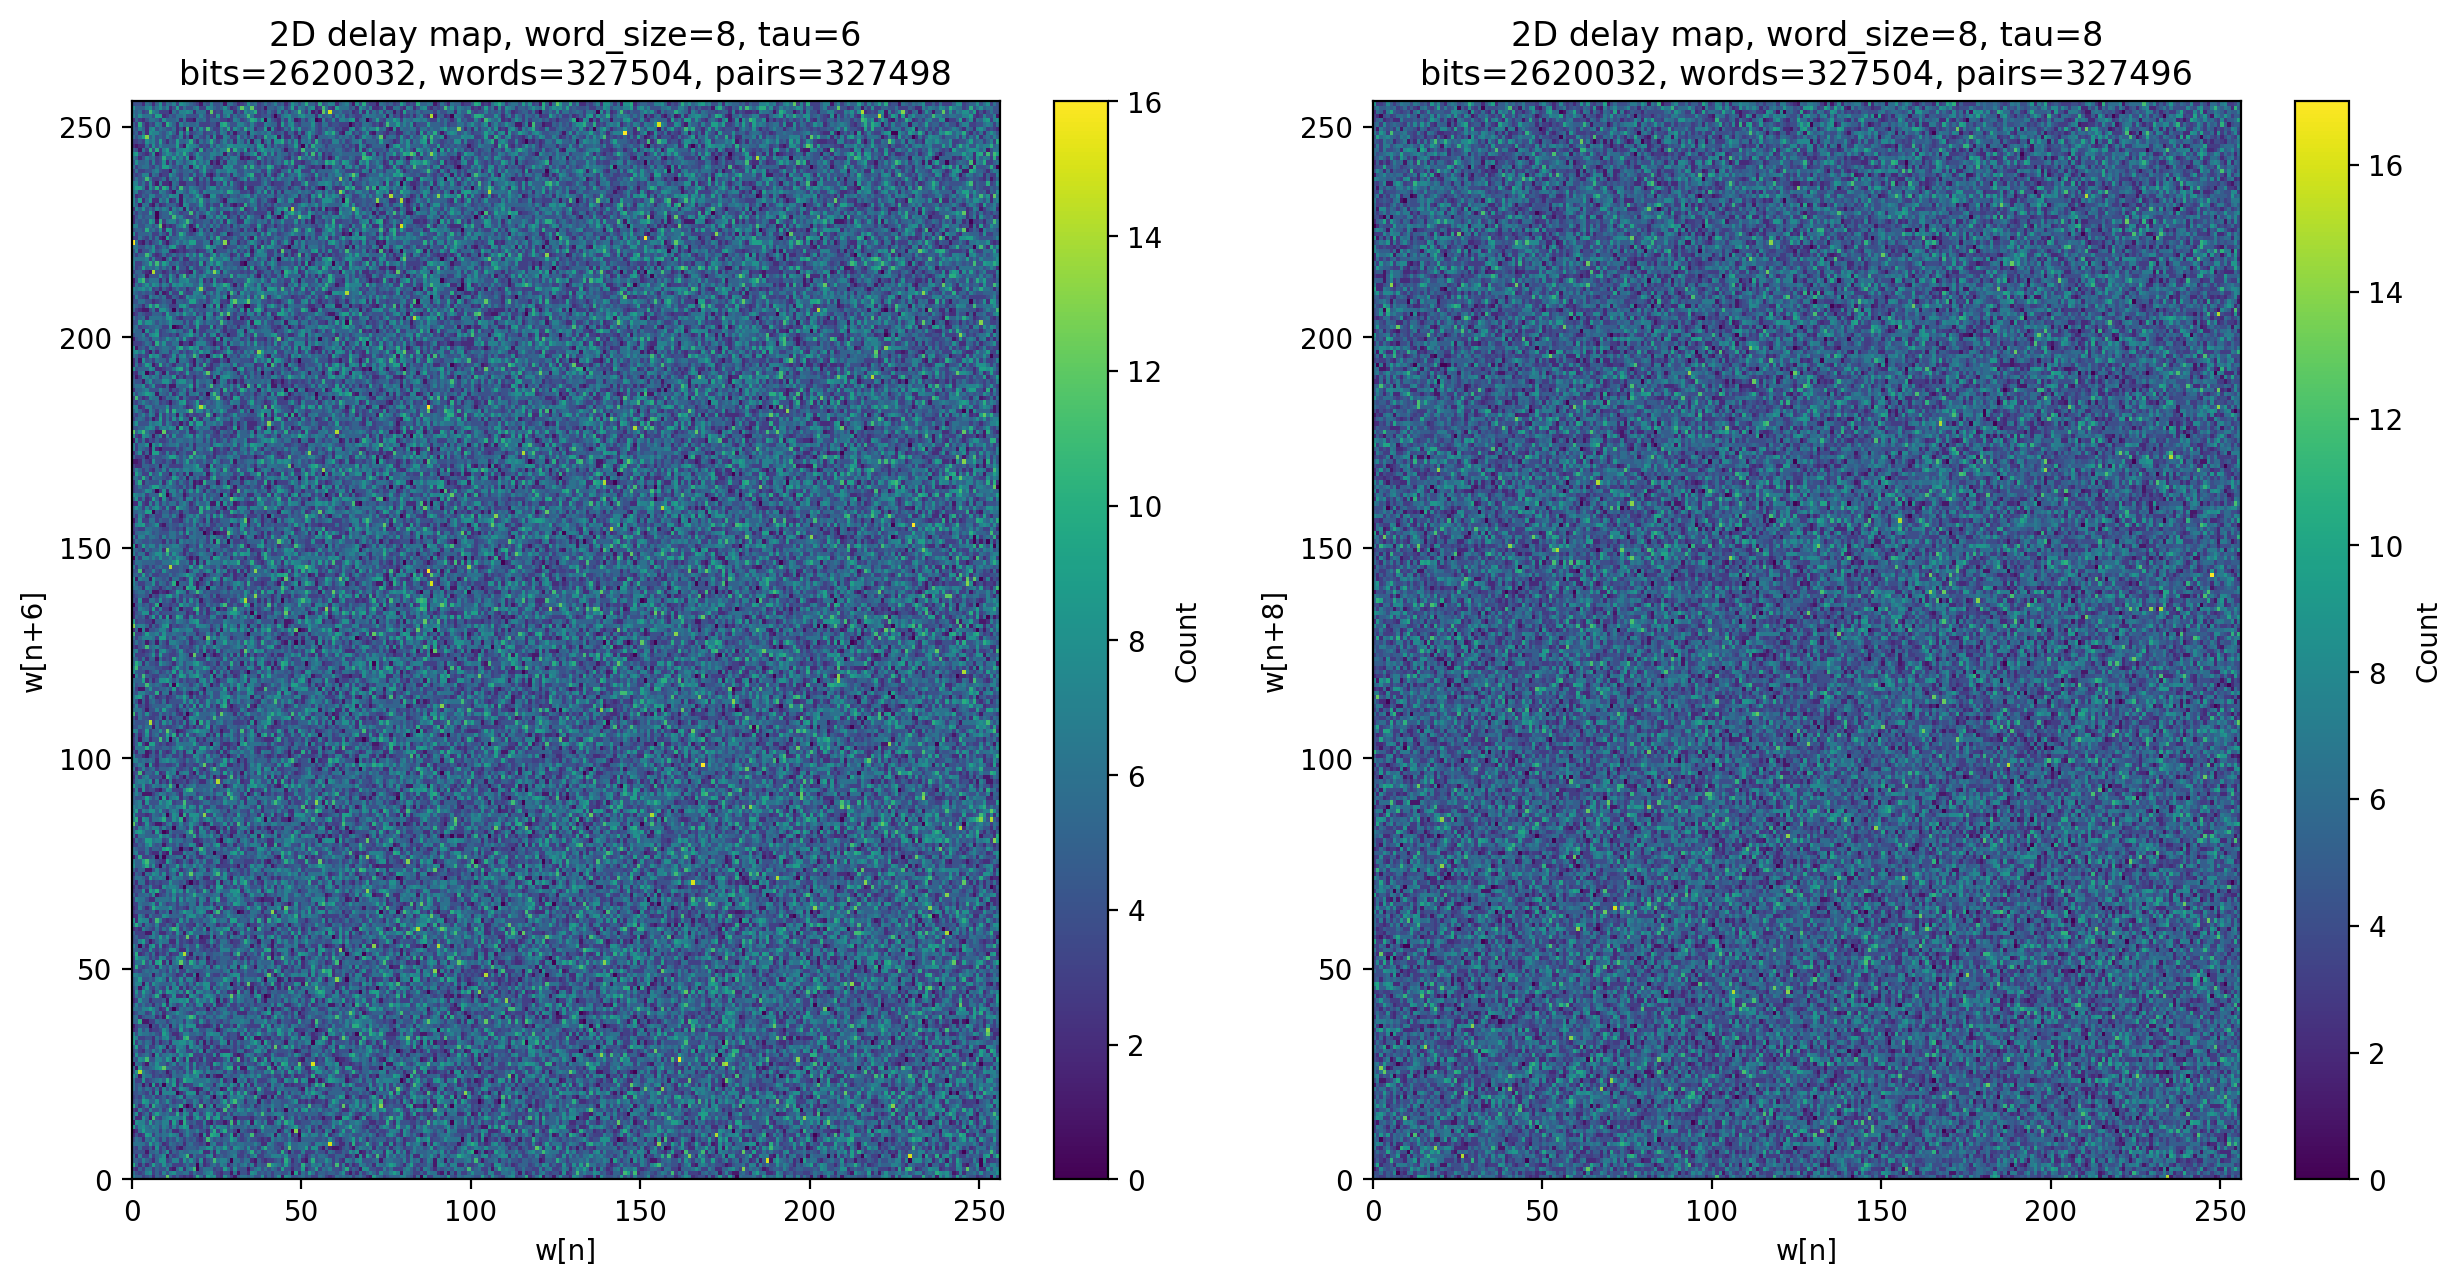
\includegraphics[width=0.98\textwidth]{gfx/vn_2d_w8_t6_t8}
    \caption{Mapy 2D dla 16 oscylatorów łączonych parami operacją XOR, po wybielaniu
    metodą von Neumanna, przy parametrach $word\_size = 8$ oraz $\tau = 6$, $\tau = 8$.}
    \label{fig:map2d_vn_w8}
\end{figure}

Mapy dla słów ośmiobitowych, przedstawione na rysunku~\ref{fig:map2d_vn_w8}, mają
charakter jednorodnego szumu bez żadnych struktur wielkoskalowych. Liczba par wynosi
w tym przypadku $327\,498$, co przy $65\,536$ komórkach daje wartość oczekiwaną zaledwie
pięciu zliczeń na komórkę. Przy tak małej liczności mapa przestaje pełnić funkcję
narzędzia pomiarowego: pojedyncze komórki puste oraz komórki o kilkunastu zliczeniach są
w tych warunkach zjawiskiem naturalnym, a nie oznaką wadliwości generatora. Widoczny
zakres skali, od zera do siedemnastu zliczeń, odpowiada odchyleniu skrajnemu rzędu pięciu
odchyleń standardowych, jednak przy $65\,536$ komórkach rozpatrywanych jednocześnie
wystąpienie takiej wartości jest oczekiwane. Mapa ta potwierdza zatem jedynie brak
struktur wielkoskalowych i nie pozwala na ilościową ocenę rozkładu.

Wynik ten wskazuje na istotne ograniczenie metody map dwuwymiarowych: użyteczna długość
słowa jest ograniczona przez długość serii pomiarowej. Aby uzyskać dla słów
ośmiobitowych liczność porównywalną z tą, jaką zapewniają słowa czterobitowe, seria
musiałaby być około dwustukrotnie dłuższa. Przy analizie strumieni poddanych wybielaniu,
skracającemu dane do jednej czwartej długości, ograniczenie to staje się szczególnie
wyraźne. Z tego względu w dalszej ocenie badanego generatora za miarodajne przyjęto
wyniki uzyskane dla słów czterobitowych, natomiast mapy dla słów ośmiobitowych
traktowano jako uzupełnienie o charakterze jakościowym.

\FloatBarrier

\section{Badanie odchylenia rozkładu bitów}

Kolejnym etapem praktycznej oceny generatora było zbadanie odchylenia rozkładu, czyli
nierównowagi pomiędzy liczbą zer i jedynek w uzyskanym strumieniu bitów. Badanie to
sprawdza, czy wyjście układu FPGA nie wykazuje przesunięcia w stronę jednej z wartości
logicznych. Jest to istotne szczególnie na etapie uruchamiania i strojenia generatora,
ponieważ asymetria może wskazywać na wpływ implementacji sprzętowej, sposobu próbkowania
lub parametrów zastosowanych oscylatorów pierścieniowych na jakość źródła entropii.

\subsection{Wyniki dla 8 oscylatorów rozmieszczonych automatycznie}

Badanie wykonano dla strumienia o długości $10\,485\,760$ bitów, pochodzącego
z~konfiguracji obejmującej osiem oscylatorów pierścieniowych rozmieszczonych
automatycznie przez narzędzie implementacyjne, bez łączenia wyjść operacją XOR
i~bez wybielania. Wyniki zestawiono w~tabeli~\ref{tab:bias_ro8}.

\begin{table}[ht]
    \centering
    \caption{Wyniki badania odchylenia rozkładu dla 8 oscylatorów rozmieszczonych
    automatycznie}
    \label{tab:bias_ro8}
    \small
    \begin{tabular}{lr}
        \toprule
        Parametr & Wartość \\
        \midrule
        Długość serii            & $10\,485\,760$ \\
        Liczba zer               & $5\,224\,958$ \\
        Liczba jedynek           & $5\,260\,802$ \\
        $P(0)$                   & $0{,}498291$ \\
        $P(1)$                   & $0{,}501709$ \\
        Bias $P(1)-0{,}5$        & $+0{,}001709$ \\
        Średnia w $\{-1,+1\}$    & $+0{,}003418$ \\
        $\sigma$                 & $1{,}54 \cdot 10^{-4}$ \\
        Odchylenie w jednostkach $\sigma$ & $11{,}1$ \\
        \bottomrule
    \end{tabular}
\end{table}

W badanym strumieniu występuje przewaga jedynek nad zerami, wynosząca $35\,844$ bity.
W~ujęciu bezwzględnym odchylenie jest niewielkie, ponieważ $P(1) = 0{,}501709$, a~więc
odstępstwo od wartości idealnej wynosi około $0{,}17\%$. Ocena istotności tego wyniku
wymaga jednak odniesienia do długości serii. Odchylenie standardowe udziału jedynek dla
źródła idealnie zrównoważonego wynosi $\sigma = 1/(2\sqrt{N}) \approx 1{,}54 \cdot
10^{-4}$, wobec czego stwierdzone odchylenie odpowiada $11{,}1$ odchylenia standardowego.

Wartość $p$ wykazana w~tabeli jako zero jest w~istocie wynikiem zaokrąglenia do sześciu
miejsc po przecinku; rzeczywista wartość jest rzędu $10^{-28}$. Oznacza to, że
prawdopodobieństwo zaobserwowania takiego odchylenia w~strumieniu pochodzącym ze źródła
idealnie zrównoważonego jest praktycznie zerowe, a~test monobitowy przy poziomie
istotności $\alpha = 0{,}01$ zostaje jednoznacznie odrzucony. Odchylenie ma zatem
charakter systematyczny i~jest cechą badanej implementacji, a~nie efektem przypadkowych
fluktuacji.

Kierunek odchylenia jest zgodny z~oczekiwaniami wynikającymi z~zasady działania
zastosowanego układu ekstrakcji entropii. Bity generowane są na podstawie detekcji zboczy,
przy czym zbocze narastające interpretowane jest jako zero, a~opadające jako jedynka.
Przewaga jedynek oznacza więc, że w~próbkowanym przebiegu częściej rejestrowane były
zbocza opadające, co odpowiada niesymetrycznemu współczynnikowi wypełnienia sygnału
z~oscylatorów. Zjawisko to wynika z~różnicy czasów propagacji zbocza narastającego
i~opadającego w~generatorach funkcji realizujących łańcuch inwerterów i~jest właściwością
technologiczną struktury układu, niezależną od sposobu opisu logiki w~języku HDL.

Uzyskany wynik wskazuje, że strumień w~postaci surowej nie spełnia wymagań stawianych
źródłom losowości i~wymaga zastosowania etapu korekcji rozkładu. Jednocześnie stwierdzone
odchylenie jest na tyle niewielkie w~ujęciu bezwzględnym, że korekcja metodą von Neumanna
powinna je usunąć przy niemal minimalnej stracie przepustowości, ponieważ udział par
odrzucanych rośnie z~kwadratem odchylenia i~dla wartości rzędu tysięcznych części pozostaje
praktycznie nierozróżnialny od przypadku granicznego. Skuteczność tego rozwiązania,
a~także wpływ liczby oscylatorów oraz łączenia ich wyjść operacją XOR na wielkość
odchylenia, przedstawiono w~kolejnych podrozdziałach.

\FloatBarrier

\subsection{Wyniki dla 8 oscylatorów rozmieszczonych ręcznie}

W kolejnej konfiguracji zachowano liczbę oscylatorów oraz długości ich łańcuchów
inwerterów, zmieniając wyłącznie sposób rozmieszczenia struktur, które narzucono ręcznie
w~oddalonych obszarach logiki programowalnej. Wyniki badania odchylenia rozkładu
zestawiono w~tabeli~\ref{tab:bias_ro8_manual}.

\begin{table}[ht]
    \centering
    \caption{Wyniki badania odchylenia rozkładu dla 8 oscylatorów rozmieszczonych ręcznie}
    \label{tab:bias_ro8_manual}
    \small
    \begin{tabular}{lr}
        \toprule
        Parametr & Wartość \\
        \midrule
        Długość serii            & $10\,485\,760$ \\
        Liczba zer               & $5\,241\,251$ \\
        Liczba jedynek           & $5\,244\,509$ \\
        $P(0)$                   & $0{,}499845$ \\
        $P(1)$                   & $0{,}500155$ \\
        Bias $P(1)-0{,}5$        & $+0{,}000155$ \\
        Średnia w $\{-1,+1\}$    & $+0{,}000311$ \\
        $\sigma$                 & $1{,}54 \cdot 10^{-4}$ \\
        Odchylenie w jednostkach $\sigma$ & $1{,}0$ \\
        Wartość $p$              & $0{,}314356$ \\
        \bottomrule
    \end{tabular}
\end{table}

Zmiana rozmieszczenia oscylatorów przyniosła bardzo wyraźną poprawę w~tej metryce.
Przewaga jedynek nad zerami zmalała z~$35\,844$ do $3\,258$ bitów, a~wartość biasu
z~$+0{,}001709$ do $+0{,}000155$, czyli ponad jedenastokrotnie. Stwierdzone odchylenie
odpowiada dokładnie jednemu odchyleniu standardowemu, a~więc mieści się w~zakresie
naturalnych fluktuacji statystycznych, jakich należy oczekiwać nawet od źródła idealnie
zrównoważonego. Potwierdza to wartość $p$ równa $0{,}314$, znacznie przewyższająca
przyjęty poziom istotności $\alpha = 0{,}01$: test monobitowy nie daje żadnych podstaw
do odrzucenia hipotezy o~zrównoważeniu strumienia.

Wynik ten jest tym bardziej wart uwagi, że kierunek odchylenia pozostał niezmieniony,
a~zmieniła się wyłącznie jego skala. Wskazuje to, że mechanizm odpowiedzialny za
asymetrię, czyli różnica czasów propagacji obu rodzajów zboczy, nie zniknął, lecz jego
wpływ na strumień wypadkowy uległ znacznemu osłabieniu. Prawdopodobnym wyjaśnieniem jest
zróżnicowanie warunków pracy poszczególnych pierścieni po ich rozproszeniu w~strukturze
układu. W~konfiguracji poprzedniej, w~której narzędzie implementacyjne umieściło wszystkie
oscylatory w~zwartym obszarze, struktury pracowały w~niemal identycznych warunkach,
wobec czego charakterystyczne dla nich odchylenia miały jednakowy kierunek i~sumowały się
w~strumieniu wyjściowym. Rozmieszczenie w~różnych obszarach struktury, obejmujących
odrębne regiony zegarowe i~różne fragmenty sieci dystrybucji zasilania, prowadzi do
zróżnicowania tych odchyleń, które w~sumie po ośmiu kanałach częściowo się kompensują.

Zestawienie tego wyniku z~wcześniejszą analizą autokorelacji prowadzi do obserwacji
istotnej dla całej pracy. Dla omawianej konfiguracji test monobitowy nie wykazuje
odstępstwa od losowości, natomiast badanie autokorelacji ujawniło w~tym samym strumieniu
zależności sięgające $270$ odchyleń standardowych, a~mapy dwuwymiarowe wyraźną
nierównomierność rozkładu wartości słów. Strumień o~praktycznie idealnie zrównoważonym
rozkładzie bitów może zatem jednocześnie zawierać silne i~łatwo wykrywalne zależności
pomiędzy kolejnymi pozycjami. Pokazuje to, że test monobitowy, choć jest naturalnym
pierwszym krokiem w~ocenie źródła losowości, bada wyłącznie rozkład brzegowy pojedynczych
bitów i~jego pozytywny wynik nie stanowi podstawy do stwierdzenia poprawności generatora.
Ocena jakości strumienia wymaga zastosowania metod badających strukturę czasową danych,
przy czym różne metody mogą prowadzić do odmiennego uszeregowania badanych konfiguracji.

\FloatBarrier

\subsection{Wyniki dla 16 oscylatorów łączonych parami operacją XOR}

W konfiguracji obejmującej szesnaście oscylatorów, których wyjścia łączone są parami
operacją XOR, badanie odchylenia rozkładu przeprowadzono na strumieniu surowym, bez
zastosowania wybielania. Wyniki zestawiono w~tabeli~\ref{tab:bias_ro16_xor}.

\begin{table}[ht]
    \centering
    \caption{Wyniki badania odchylenia rozkładu dla 16 oscylatorów łączonych parami
    operacją XOR}
    \label{tab:bias_ro16_xor}
    \small
    \begin{tabular}{lr}
        \toprule
        Parametr & Wartość \\
        \midrule
        Długość serii            & $10\,485\,760$ \\
        Liczba zer               & $5\,241\,014$ \\
        Liczba jedynek           & $5\,244\,746$ \\
        $P(0)$                   & $0{,}499822$ \\
        $P(1)$                   & $0{,}500178$ \\
        Bias $P(1)-0{,}5$        & $+0{,}000178$ \\
        Średnia w $\{-1,+1\}$    & $+0{,}000356$ \\
        $\sigma$                 & $1{,}54 \cdot 10^{-4}$ \\
        Odchylenie w jednostkach $\sigma$ & $1{,}2$ \\
        Wartość $p$              & $0{,}249115$ \\
        \bottomrule
    \end{tabular}
\end{table}

Odnotowana przewaga jedynek nad zerami wynosi $3\,732$ bity, a~wartość biasu
$+0{,}000178$, co odpowiada $1{,}2$ odchylenia standardowego. Wartość $p$ równa $0{,}249$
znacznie przewyższa przyjęty poziom istotności, wobec czego test monobitowy nie daje
podstaw do odrzucenia hipotezy o~zrównoważeniu strumienia.

Wynik ten jest praktycznie identyczny z~uzyskanym dla konfiguracji z~ośmioma oscylatorami
rozmieszczonymi ręcznie, gdzie bias wyniósł $+0{,}000155$, czyli $1{,}0$ odchylenia
standardowego. Różnica między obiema wartościami mieści się w~granicach naturalnego
rozrzutu i~nie pozwala stwierdzić, która konfiguracja jest w~tej metryce lepsza.
Obserwacja ta wymaga komentarza, ponieważ na pierwszy rzut oka pozostaje w~sprzeczności
z~oczekiwaniem teoretycznym. Połączenie dwóch niezależnych źródeł operacją XOR powinno
prowadzić do zmniejszenia odchylenia w~sposób multiplikatywny: przy odchyleniach
$\varepsilon_1$ oraz $\varepsilon_2$ odchylenie sygnału wynikowego wynosi
$2\varepsilon_1\varepsilon_2$, wobec czego dla wartości rzędu tysięcznych części
oczekiwane odchylenie po operacji XOR powinno być mniejsze o~kilka rzędów wielkości.

Wyjaśnieniem tej rozbieżności jest fakt, że dla obu konfiguracji stwierdzone odchylenie
znajduje się już na poziomie naturalnego rozrzutu statystycznego wyznaczonego długością
serii. Odchylenie standardowe $\sigma \approx 1{,}54 \cdot 10^{-4}$ stanowi w~tym
przypadku granicę czułości pomiaru: nawet gdyby operacja XOR zredukowała odchylenie
rzeczywiste do wartości pomijalnie małej, zmierzony bias pozostałby na poziomie rzędu
jednego $\sigma$, ponieważ wynikałby wówczas wyłącznie z~losowego rozrzutu liczby jedynek
w~skończonej próbie. Test monobitowy nie jest zatem zdolny rozróżnić tych dwóch
konfiguracji przy zastosowanej długości serii, a~stwierdzenie rzeczywistej poprawy
wymagałoby zebrania danych o~kilka rzędów wielkości dłuższych.

Niezależne potwierdzenie bardzo małego odchylenia dla omawianej konfiguracji przynosi
natomiast wydajność wybielania metodą von Neumanna, omówiona w~podrozdziale dotyczącym
autokorelacji. Udział bitów zachowanych po korekcji wyniósł $24{,}99\%$, a~więc
praktycznie tyle, ile wynosi granica teoretyczna dla źródła nieobciążonego. Ponieważ
udział par odrzucanych rośnie z~kwadratem odchylenia, wskaźnik ten jest czuły na bias
i~jego wartość potwierdza, że rzeczywiste odchylenie strumienia było w~tej konfiguracji
istotnie mniejsze, niż wskazuje sam wynik testu monobitowego.

Podsumowując, trzy z~czterech badanych konfiguracji różnią się w~zakresie odchylenia
rozkładu w~sposób jednoznaczny jedynie w~jednym przypadku: automatyczne rozmieszczenie
oscylatorów prowadziło do odchylenia na poziomie $11$ odchyleń standardowych, natomiast
wszystkie konfiguracje z~rozmieszczeniem ręcznym dają wyniki nierozróżnialne od źródła
zrównoważonego. Decydującym czynnikiem w~tej metryce okazało się zatem rozproszenie
struktur w~obrębie układu, a~nie liczba oscylatorów ani zastosowanie operacji XOR.

\FloatBarrier

\subsection{Wyniki dla 16 oscylatorów z wybielaniem metodą von Neumanna}

Ostatni pomiar wykonano dla tej samej serii pomiarowej co poprzednio, poddanej wybielaniu
metodą von Neumanna. Wyniki zestawiono w~tabeli~\ref{tab:bias_ro16_vn}.

\begin{table}[ht]
    \centering
    \caption{Wyniki badania odchylenia rozkładu dla 16 oscylatorów łączonych parami
    operacją XOR, po wybielaniu metodą von Neumanna}
    \label{tab:bias_ro16_vn}
    \small
    \begin{tabular}{lr}
        \toprule
        Parametr & Wartość \\
        \midrule
        Długość serii            & $2\,620\,032$ \\
        Liczba zer               & $1\,308\,483$ \\
        Liczba jedynek           & $1\,311\,549$ \\
        $P(0)$                   & $0{,}499415$ \\
        $P(1)$                   & $0{,}500585$ \\
        Bias $P(1)-0{,}5$        & $+0{,}000585$ \\
        Średnia w $\{-1,+1\}$    & $+0{,}001170$ \\
        $\sigma$                 & $3{,}09 \cdot 10^{-4}$ \\
        Odchylenie w jednostkach $\sigma$ & $1{,}9$ \\
        Wartość $p$              & $0{,}058203$ \\
        \bottomrule
    \end{tabular}
\end{table}

Test monobitowy przy poziomie istotności $\alpha = 0{,}01$ nie daje podstaw do odrzucenia
hipotezy o~zrównoważeniu strumienia, ponieważ wartość $p$ wynosi $0{,}058$. Wynik ten
wymaga jednak uważniejszej interpretacji, gdyż w~ujęciu bezwzględnym wartość biasu
wzrosła: z~$+0{,}000178$ dla strumienia surowego do $+0{,}000585$ po wybielaniu, a~więc
ponad trzykrotnie. Jest to obserwacja sprzeczna z~przeznaczeniem zastosowanej metody,
która ma odchylenie rozkładu usuwać, a~nie zwiększać.

Zasadnicza część tej rozbieżności ma charakter pozorny i~wynika ze skrócenia serii.
Wybielanie zredukowało długość strumienia do jednej czwartej, wobec czego odchylenie
standardowe wzrosło dwukrotnie, do $\sigma \approx 3{,}09 \cdot 10^{-4}$. Wyrażone
w~jednostkach naturalnego rozrzutu odchylenie wynosi zatem $1{,}9$ zamiast $1{,}2$,
a~więc wzrost jest znacznie mniej wyraźny niż w~ujęciu bezwzględnym i~mieści się
w~zakresie, jakiego można oczekiwać przy losowym rozrzucie. Porównywanie wartości biasu
pomiędzy seriami o~różnej długości bez takiego przeliczenia prowadziłoby do błędnych
wniosków, ponieważ każde skrócenie danych z~definicji zwiększa oczekiwaną wartość
bezwzględną zmierzonego odchylenia.

Pozostaje jednak pytanie, dlaczego wybielanie nie doprowadziło do wartości bliższej zeru,
skoro metoda von Neumanna gwarantuje idealne zrównoważenie strumienia wyjściowego.
Gwarancja ta obowiązuje wyłącznie przy założeniu wzajemnej niezależności kolejnych bitów
strumienia wejściowego. Tymczasem analiza autokorelacji wykazała dla tej konfiguracji
istnienie zależności w~zakresie małych opóźnień, przekraczających pięć odchyleń
standardowych. Przy skorelowanym strumieniu wejściowym pary o~różnych wartościach
przestają występować z~jednakowym prawdopodobieństwem, w~konsekwencji czego korekcja nie
usuwa odchylenia w~pełni. Stwierdzone po wybielaniu odchylenie na poziomie dwóch
odchyleń standardowych należy zatem traktować jako pośredni ślad zależności czasowych
obecnych w~strumieniu surowym, a~nie jako niedoskonałość samej implementacji korekcji.

Warto przy tym zauważyć, że mimo braku pełnego usunięcia odchylenia wybielanie
poprawiło wynik pozostałych zastosowanych metod: mapy dwuwymiarowe wykazały spadek
rozrzutu zliczeń z~około sześciu do niespełna trzech odchyleń standardowych, a~przebieg
autokorelacji utracił uporządkowaną strukturę. Metoda von Neumanna okazała się więc
skuteczna wobec tych odstępstw od losowości, których nie wykrywa test monobitowy,
pozostając jednocześnie bez wyraźnego wpływu na samą wielkość odchylenia rozkładu, która
w~konfiguracjach z~ręcznym rozmieszczeniem oscylatorów była już przed korekcją
nierozróżnialna od naturalnego rozrzutu.

\FloatBarrier

\section{Wnioski z analizy statystycznej generatora liczb losowych}

Przeprowadzona analiza objęła trzy metody: badanie autokorelacji strumienia bitów, mapy
dwuwymiarowe rozkładu słów oraz test odchylenia rozkładu bitów. Każdą z nich zastosowano
do czterech konfiguracji generatora, różniących się liczbą oscylatorów pierścieniowych,
sposobem ich rozmieszczenia w~strukturze układu, obecnością operacji XOR na wyjściach oraz
zastosowaniem korekcji metodą von Neumanna. Zestawienie uzyskanych wyników przedstawiono
w~tabeli~\ref{tab:synteza}, przy czym wszystkie wartości wyrażono w~jednostkach odchylenia
standardowego właściwego dla danej metody i~długości serii, co umożliwia porównywanie
pomiarów o~różnej liczności.

\begin{table}[htbp]
    \centering
    \caption{Zestawienie wyników wszystkich zastosowanych metod analizy. Wartości
    wyrażono w~jednostkach odchylenia standardowego}
    \label{tab:synteza}
    \small
    \begin{tabular}{clccc}
        \toprule
        Nr & Konfiguracja & Odchylenie rozkładu & Autokorelacja & Mapy 2D \\
        \midrule
        1 & 8 RO, rozmieszczenie automatyczne & $11{,}1$ & $3{,}8$   & $8{,}5$ \\
        2 & 8 RO, rozmieszczenie ręczne       & $1{,}0$  & $270$     & $67$ \\
        3 & 16 RO, XOR                        & $1{,}2$  & $9{,}8$   & $6$ \\
        4 & 16 RO, XOR, von Neumann           & $1{,}9$  & $3{,}2$   & $2{,}7$ \\
        \bottomrule
    \end{tabular}
\end{table}

Najistotniejszym wnioskiem wynikającym z~tego zestawienia jest brak zgodności pomiędzy
zastosowanymi metodami co do uszeregowania badanych konfiguracji. Konfiguracja pierwsza,
w~której oscylatory rozmieszczono automatycznie, wypadła najlepiej w~badaniu
autokorelacji, a~jednocześnie zdecydowanie najgorzej w~teście odchylenia rozkładu, gdzie
odnotowane odstępstwo sięgnęło jedenastu odchyleń standardowych i~doprowadziło do
odrzucenia hipotezy o~zrównoważeniu strumienia. Konfiguracja druga wykazała zależność
odwrotną: rozproszenie struktur zredukowało odchylenie rozkładu do poziomu naturalnych
fluktuacji, jednocześnie pogarszając wynik autokorelacji o~blisko dwa rzędy wielkości.
Żadna z~pojedynczych metod nie pozwoliłaby zatem na poprawną ocenę badanego źródła,
a~oparcie wniosków wyłącznie na teście monobitowym doprowadziłoby do zaakceptowania
strumienia zawierającego zależności czasowe wykrywalne na poziomie dwustu siedemdziesięciu
odchyleń standardowych.

Rozproszenie oscylatorów w~strukturze układu okazało się czynnikiem decydującym dla
odchylenia rozkładu. Wszystkie trzy konfiguracje z~rozmieszczeniem ręcznym dały wyniki
nierozróżnialne od źródła zrównoważonego, mieszczące się w~przedziale od jednego do dwóch
odchyleń standardowych, wobec jedenastu odchyleń dla rozmieszczenia automatycznego.
Wyjaśnieniem jest zróżnicowanie warunków pracy poszczególnych pierścieni: struktury
umieszczone w~zwartym obszarze pracują w~niemal identycznych warunkach temperaturowych
i~zasilania, wobec czego charakterystyczne dla nich asymetrie czasów propagacji zboczy
mają jednakowy kierunek i~sumują się w~strumieniu wypadkowym, natomiast po rozproszeniu
częściowo się kompensują. Ten sam zabieg pogorszył jednak wynik autokorelacji, ponieważ
zróżnicowanie lokalnych warunków pracy przekłada się na większy rozrzut częstotliwości
oscylatorów, a~przy stałej kolejności zapisu kanałów do bufora prowadzi to do powstania
wyraźniejszej struktury okresowej w~strumieniu wyjściowym.

Zwiększenie liczby oscylatorów do szesnastu wraz z~łączeniem ich wyjść operacją XOR
przyniosło znaczącą poprawę wyników obu metod badających strukturę danych: amplituda
zależności autokorelacyjnych zmalała blisko dwudziestoośmiokrotnie, a~rozrzut zliczeń na
mapach dwuwymiarowych z~sześćdziesięciu siedmiu do sześciu odchyleń standardowych. W~teście
odchylenia rozkładu nie stwierdzono natomiast różnicy względem konfiguracji poprzedniej,
co nie oznacza braku poprawy, lecz wynika z~ograniczonej czułości pomiaru: przy serii
o~długości $10\,485\,760$ bitów odchylenie standardowe wynosi $1{,}54 \cdot 10^{-4}$
i~stanowi granicę rozdzielczości, poniżej której test monobitowy nie różnicuje źródeł.
Pośrednim potwierdzeniem bardzo małego odchylenia dla tej konfiguracji jest wydajność
korekcji von Neumanna, wynosząca $24{,}99\%$ długości wejściowej, a~więc praktycznie równa
granicy teoretycznej osiąganej dla źródła nieobciążonego.

Zastosowanie korekcji metodą von Neumanna okazało się skuteczne wobec tych odstępstw od
losowości, których test monobitowy nie wykrywa. Po wybielaniu przebieg autokorelacji
utracił uporządkowaną strukturę obejmującą opóźnienia od dwóch do sześciu, a~rozrzut
zliczeń na mapach dwuwymiarowych spadł do poziomu poniżej trzech odchyleń standardowych,
zgodnego z~oczekiwaniem dla rozkładu równomiernego. Metoda nie zmniejszyła natomiast
samego odchylenia rozkładu, które pozostało na poziomie dwóch odchyleń standardowych.
Wynika to z~faktu, że korekcja von Neumanna gwarantuje zrównoważenie strumienia
wyjściowego wyłącznie przy założeniu wzajemnej niezależności bitów wejściowych, a~założenie
to nie było w~badanym strumieniu spełnione. Stwierdzone po wybielaniu odchylenie należy
zatem traktować jako pośredni ślad zależności czasowych obecnych w~danych surowych.

Analiza wskazała jednocześnie źródło zasadniczej części wykrytych odstępstw. We wszystkich
konfiguracjach zależności koncentrowały się w~zakresie opóźnień odpowiadających liczbie
kanałów doprowadzonych do modułu ekstrakcji entropii oraz długości bajtu, a~ich charakter
zmieniał się wraz z~relacjami częstotliwości pomiędzy oscylatorami, nie zaś wraz z~jakością
samych źródeł szumu. Wskazuje to na warstwę serializacji jako mechanizm odpowiedzialny za
powstawanie struktury okresowej: bity zapisywane są do bufora w~stałej kolejności numerów
kanałów, wobec czego uporządkowanie oscylatorów według częstotliwości pracy przekłada się
bezpośrednio na uporządkowanie wartości w~strumieniu wyjściowym.

Przy formułowaniu powyższych wniosków należy uwzględnić dwa ograniczenia przyjętej
metodyki. Przejście od konfiguracji drugiej do trzeciej obejmowało jednoczesną zmianę dwóch
parametrów, liczby oscylatorów oraz obecności operacji XOR, w~związku z~czym nie jest
możliwe rozdzielenie wpływu każdego z~nich na obserwowaną poprawę.

Jako kierunki dalszych prac zasadne wydają się trzy zagadnienia. Pierwszym jest
weryfikacja hipotezy o~serializacji poprzez rozdzielenie zarejestrowanego strumienia na
podstrumienie odpowiadające poszczególnym kanałom i~zbadanie każdego z~nich osobno, co
pozwoliłoby stwierdzić, czy zależności powstają w~pojedynczych oscylatorach, czy dopiero
przy ich łączeniu. Drugim jest modyfikacja samego mechanizmu serializacji, na przykład
przez wprowadzenie zmiennej kolejności zapisu kanałów do bufora, co powinno usunąć
zależności okresowe u~ich źródła, bez ponoszenia kosztu przepustowości właściwego dla
korekcji von Neumanna. Trzecim jest przeniesienie korekcji do struktury układu FPGA
i~umieszczenie jej bezpośrednio przed nadajnikiem, co pozwoliłoby uzyskać strumień
o~poprawionych właściwościach statystycznych bez konieczności przetwarzania danych po
stronie komputera.

\FloatBarrier